% !TeX document-id = {4c50d318-ae06-42ec-8e3f-7706d393a431}
% !TeX spellcheck = sl_SI
% !TeX program = pdflatex+bibtex+makeindex
% vim: set spell spelllang=sl:
%& -job-name=newfilenameialwayswanted
% za preverjanje črkovanja, če se uporablja Texstudio ali vim
\documentclass[12pt,a4paper,twoside]{article}
\usepackage[utf8]{inputenc}  % pravilno razpoznavanje unicode znakov

% NASLEDNJE UKAZE USTREZNO POPRAVI
\newcommand{\program}{Matematika} % ime studijskega programa
\newcommand{\imeavtorja}{Gašper Domen Romih} % ime avtorja
\newcommand{\imementorja}{prof.~dr.~Nino Bašić} % akademski naziv in ime mentorja, uporabi poln naziv, prof.~dr.~, doc.~dr., ali izr.~prof.~dr.
\newcommand{\imesomentorja}{} % akademski naziv in ime somentorja, če ga imate
\newcommand{\naslovdela}{Domneva 1-2-3}
\newcommand{\letnica}{2020} % letnica magistriranja
\newcommand{\opis}{Delo obravnava domnevo 1-2-3 ter njene variacije.}  % Opis dela v eni povedi. Ne sme vsebovati matematičnih simbolov v $ $.
\newcommand{\kljucnebesede}{teorija grafov\sep kombinatorika} % ključne besede, ločene z \sep, da se PDF metapodatki prav procesirajo
\newcommand{\keywords}{integration\sep complex} % ključne besede v angleščini
\newcommand{\organization}{Univerza v Ljubljani, Fakulteta za matematiko in fiziko} % fakulteta
\newcommand{\literatura}{literatura}  % pot do datoteke z literaturo (brez .bib končnice)
\newcommand{\sep}{, }  % separator med ključnimi besedami v besedilu
% KONEC PODATKOV

\usepackage{bibentry}         % za navajanje literature v programu dela s celim imenom
\nobibliography{\literatura}
\newcommand{\plancite}[1]{\item[\cite{#1}] \bibentry{#1}} % citiranje v programu dela

\usepackage{filecontents}  % za pisanje datoteke s PDF metapodatki
\usepackage{silence} \WarningFilter{latex}{Overwriting file}  % odstrani annoying warning o obstoju datoteke
% datoteka s PDF metapodatki, zgenerira se kot magisterij.xmpdata
\begin{filecontents*}{\jobname.xmpdata}
  \Title{\naslovdela}
  \Author{\imeavtorja}
  \Keywords{\kljucnebesede}
  \Subject{\opis}
  \Org{\organization}
\end{filecontents*}

\usepackage[a-1b]{pdfx}  % zgenerira PDF v tem PDF/A-1b formatu, kot zahteva knjižnica
\hypersetup{bookmarksopen, bookmarksdepth=3, colorlinks=true,
  linkcolor=black, anchorcolor=black, citecolor=black, filecolor=black,
  menucolor=black, runcolor=black, urlcolor=black, pdfencoding=auto,
  breaklinks=true, psdextra}

\usepackage[slovene]{babel}  % slovenščina
\usepackage[T1]{fontenc}     % naprednejše kodiranje fonta
\usepackage{amsmath,amssymb,amsfonts,amsthm} % matematični paketi
\usepackage{graphicx}     % za slike
\usepackage{mathtools}
\usepackage[numbers]{natbib}
%\usepackage[dvipsnames,usenames]{color} % barve
\usepackage{emptypage}    % prazne strani so neoštevilčene, ampak so štete
\usepackage{units}        % fizikalne enote kot \unit[12]{kg} z polovico nedeljivega presledka, glej primer v kodi
\usepackage{makeidx}      % za stvarno kazalo, lahko zakomentiraš, če ne rabiš
\makeindex                % za stvarno kazalo, lahko zakomentiraš, če ne rabiš
% oblika strani
\usepackage[
  top=3cm,
  bottom=3cm,
  inner=3.5cm,      % margini za dvostransko tiskanje
  outer=2.5cm,
  footskip=40pt     % pozicija številke strani
]{geometry}

% VEČ ZANIMIVIH PAKETOV
% \usepackage{array}      % več možnosti za tabele
% \usepackage[list=true,listformat=simple]{subcaption}  % več kot ena slika na figure, omogoči slika 1a, slika 1b
% \usepackage[all]{xy}    % diagrami
% \usepackage{doi}        % za clickable DOI entrye v bibliografiji
% \usepackage{enumerate}     % več možnosti za sezname

% Za barvanje source kode
% \usepackage{minted}
% \renewcommand\listingscaption{Program}

% Za pisanje psevdokode
% \usepackage{algpseudocode}  % za psevdokodo
% \usepackage{algorithm}
% \floatname{algorithm}{Algoritem}
% \renewcommand{\listalgorithmname}{Kazalo algoritmov}

% DRUGI TVOJI PAKETI:
% tukaj
\usepackage{tikz}


\usetikzlibrary{quotes} % LATEX and plain TEX
\usetikzlibrary{arrows,automata,positioning}

\usetikzlibrary{shapes.geometric}
\usepackage{subcaption}
\usepackage{mwe}
\usepackage{float}
\usepackage[]{algorithm2e}



\setlength{\overfullrule}{50pt} % označi predlogo vrstico
\pagestyle{plain}               % samo številka strani na dnu, nobene glave / noge

% ukazi za matematična okolja
\theoremstyle{definition} % tekst napisan pokončno
\newtheorem{definicija}{Definicija}[section]
\newtheorem{primer}[definicija]{Primer}
\newtheorem{opomba}[definicija]{Opomba}
\newtheorem{aksiom}{Aksiom}
\newtheorem{domneva}[definicija]{Domneva}

\theoremstyle{plain} % tekst napisan poševno
\newtheorem{lema}[definicija]{Lema}
\newtheorem{izrek}[definicija]{Izrek}
\newtheorem{trditev}[definicija]{Trditev}
\newtheorem{posledica}[definicija]{Posledica}


\newcommand{\ec}{\chi_{\Sigma}^e}
\newcommand{\ect}{\chi_{\Sigma}^t}
\newcommand{\ecl}{ch_{\Sigma}^e}
\newcommand{\eclt}{ch_{\Sigma}^t}

\numberwithin{equation}{section}  % števec za enačbe zgleda kot (2.7) in se resetira v vsakem poglavju

% Matematični ukazi
\newcommand{\R}{\mathbb R}
\newcommand{\N}{\mathbb N}
\newcommand{\Z}{\mathbb Z}
\newcommand{\C}{\mathbb C}
\newcommand{\Q}{\mathbb Q}
\newcommand{\var}{\texttt}

\graphicspath{{slike/}}



% \DeclareMathOperator{\tr}{tr}  % morda potrebuješ operator za sled ali kaj drugega?

\DeclareMathOperator{\per}{per}
\DeclareMathOperator{\mind}{mind}
\DeclareMathOperator{\tmind}{tmind}
\DeclareMathOperator{\pind}{pind}
\DeclareMathOperator{\arctg}{arctg}
\DeclareMathOperator{\col}{col}
\DeclareMathOperator{\ch}{ch}
\DeclareMathOperator{\s}{s}

% bold matematika znotraj \textbf{ }, tudi v naslovih, kot \omega spodaj
\makeatletter \g@addto@macro\bfseries{\boldmath} \makeatother

% Poimenuj kazalo slik kot ``Kazalo slik'' in ne ``Slike''
\addto\captionsslovene{
  \renewcommand{\listfigurename}{Kazalo slik}%
}

% če želiš, da se poglavja začnejo na lihih straneh zgoraj
% \let\oldsection\section
% \def\section{\cleardoublepage\oldsection}

%%%%%%%%%%%%%%%%%%%%%%%%%%%%%%%%%%%%%%%%%%
%%%%%%           DOCUMENT           %%%%%%
%%%%%%%%%%%%%%%%%%%%%%%%%%%%%%%%%%%%%%%%%%

\begin{document}

\pagenumbering{roman} % začnemo z rimskimi številkami
\thispagestyle{empty} % ampak na prvi strani ni številke

\noindent{\large
UNIVERZA V LJUBLJANI\\[1mm]
FAKULTETA ZA MATEMATIKO IN FIZIKO\\[5mm]
\program\ -- 2.~stopnja}
% ustrezno dopolni za IŠRM
\vfill

\begin{center}
  \large
  \imeavtorja\\[3mm]
  \Large
  \textbf{\MakeUppercase{\naslovdela}}\\[10mm]
  \large
  Magistrsko delo \\[1cm]
  Mentor: \imementorja \\[2mm] % ustrezno popravi spol
%   Somentor: \imesomentorja   % dodaj, če potrebno
\end{center}
\vfill

\noindent{\large Ljubljana, \letnica}

\cleardoublepage

%% IZJAVA O AVTORSTVU
%\pdfbookmark[1]{Izjava o avtorstvu}{izjava} % bookmark v PDF, \pdfbookmark[nivo]{text}{label}
%
%% izjava: po potrebi spremeni v žensko obliko
%\setlength\topsep{0pt}
%\setlength\parskip{0pt}
%\begin{center}
%  \textbf{Univerza v Ljubljani} \\
%  \textbf{Fakulteta za matematiko in fiziko}
%
%  \vfill
%
%  \underline{Izjava o avtorstvu, istovetnosti tiskane in elektronske verzije magistrskega dela in} \\
%  \underline{objavi osebnih podatkov študenta}
%
%  \vfill
%
%  \setlength\topsep{0pt}
%  \setlength\parskip{0pt}
%  \begin{flushleft}
%    Spodaj podpisani študent \imeavtorja{} avtor magistrskega dela (v nadaljevanju: pisnega
%    zaključnega dela študija) z naslovom:
%  \end{flushleft}
%
%  \vfill
%
%  \textbf{\naslovdela}
%
%  \vfill
%
%  IZJAVLJAM
%\end{center}
%
%\begin{enumerate}[1. ]
%  \item \emph{Obkrožite eno od variant a) ali b)}
%  \begin{enumerate}[a)]
%    \item da sem pisno zaključno delo študija izdelal samostojno;
%    \item da je pisno zaključno delo študija rezultat lastnega dela več kandidatov in izpolnjuje
%      pogoje, ki jih Statut UL določa za skupna zaključna dela študija ter je v zahtevanem deležu
%      rezultat mojega samostojnega dela;
%  \end{enumerate}
%  pod mentorstvom IZPOLNI. % dopiši \imementorja v rodilniku
%%   \\ in somentorstvom IZPOLNI. % dopiši \imesomentorja v rodilniku
%  \item da je tiskana oblika pisnega zaključnega dela študija istovetna elektronski obliki
%    pisnega zaključnega dela študija;
%  \item da sem pridobil vsa potrebna dovoljenja za uporabo podatkov in avtorskih del v pisnem
%    zaključnem delu študija in jih v pisnem zaključnem delu študija jasno označil;
%  \item da sem pri pripravi pisnega zaključnega dela študija ravnal v skladu z etičnimi načeli in,
%    kjer je to potrebno, za raziskavo pridobil soglasje etične komisije;
%  \item da soglašam, da se elektronska oblika pisnega zaključnega dela študija uporabi za preverjanje
%    podobnosti vsebine z drugimi deli s programsko  opremo za preverjanje podobnosti
%    vsebine, ki je povezana s študijskim informacijskim sistemom fakultete;
%  \item da na UL neodplačno, neizključno, prostorsko in časovno neomejeno prenašam pravico shranitve
%    avtorskega dela v elektronski obliki, pravico reproduciranja ter pravico dajanja pisnega
%    zaključnega dela študija na voljo javnosti na svetovnem spletu preko Repozitorija UL;
%  \item da dovoljujem objavo svojih osebnih podatkov, ki so navedeni v pisnem zaključnem delu študija
%    in tej izjavi, skupaj z objavo pisnega zaključnega dela študija.
%\end{enumerate}
%
%\vfill
%
%\noindent
%Kraj:  \hfill   Podpis študenta: \phantom{prostor za podpis}
%
%\vfill
%
%\noindent
%Datum:
%
%\cleardoublepage
%% END IZJAVA O AVTORSTVU

% zahvala
\pdfbookmark[1]{Zahvala}{zahvala} %
\section*{Zahvala}
Neobvezno.
Zahvaljujem se \dots
% end zahvala -- izbriši vse med zahvala in end zahvala, če je ne rabiš

\cleardoublepage

\pdfbookmark[1]{\contentsname}{kazalo-vsebine}
\tableofcontents

% list of figures
% \cleardoublepage
% \pdfbookmark[1]{\listfigurename}{kazalo-slik}
% \listoffigures
% end list of figures

\cleardoublepage

\section*{Program dela}
\addcontentsline{toc}{section}{Program dela} % dodajmo v kazalo
Tu naj bi mentor napisal program dela, skupaj z osnovno literaturo spodaj. To je v template-u, ki ga iamo na spletni učilnici za seminar. Verjetno tega ni v končno verziji. Okviren osnutek z povezavami na določene reference bom napisal kar v glavnem delu dokumenta.

\section*{Osnovna literatura}
Literatura mora biti tukaj posebej samostojno navedena (po pomembnosti) in ne
le citirana. V tem razdelku literature ne oštevilčimo po svoje, ampak uporabljamo
okolje itemize in ukaz plancite, saj je celotna literatura oštevilčena na koncu.
\begin{itemize}
  \plancite{maingraph}
  \plancite{base}
  \plancite{regular}
  \plancite{examples}
  \plancite{proof12345}
\end{itemize}

\vspace{2cm}
\hspace*{\fill} Podpis mentorja: \phantom{prostor za podpis}

% \vspace{2cm}
% \hspace*{\fill} Podpis somentorja: \phantom{prostor za podpis}

\cleardoublepage
\pdfbookmark[1]{Povzetek}{abstract}

\begin{center}
\textbf{\naslovdela} \\[3mm]
\textsc{Povzetek} \\[2mm]
\end{center}
Povezavam grafa $G$ priredimo uteži z vrednostmi $1,2,\ldots,k$. Uteži na povezavah porodijo pravilno barvanje grafa $G$, če se vsote uteži incedenčnih povezav razlikujejo za vsaki sosednji vozlišči. V nalogi se osredotočimo na zgornjo mejo za $k$ za splošne grafe. Obravnavamo tudi polne ter $d$-regularne grafe. 

\vfill
\begin{center}
\textbf{English translation of the title} \\[3mm] % prevod slovenskega naslova dela
\textsc{Abstract}\\[2mm]
\end{center}

An abstract of the work is written here. This includes a short description of
the content and not the structure of your work.

\vfill\noindent
\textbf{Math.~Subj.~Class.~(2010):} oznake kot 74B05, 65N99, na voljo so na naslovu
\url{http://www.ams.org/msc/msc2010.html?t=65Mxx} \\[1mm]
\textbf{Ključne besede:} \kljucnebesede \\[1mm]
\textbf{Keywords:} \keywords

\cleardoublepage

\setcounter{page}{1}    % od sedaj naprej začni zopet z 1
\pagenumbering{arabic}  % in z arabskimi številkami

\section{Uvod}
Motivacija za domnevo 1-2-3 izhaja iz t.i.\ iregularnostne moči grafa, ki si jo intuitivno lahko predstavljamo kot neko mero, ki nam pove, koliko nekemu grafu manjka do tega, da postane regularen. Pri tem so regularni grafi taki grafi, kjer imajo vsa vozlišča enako število sosedov oz.\ imajo enako stopnjo. Na preprost način lahko ugotovimo, da obstajajo regularni grafi vseh redov. Zanima nas, če lahko karakteriziramo grafe, ki se od regularnih najbolj razlikujejo in sicer tako, da zahtevamo različne stopnje za vsa vozlišča v grafu. Vendar nam preprosto dejstvo o grafih pove, da imata vsaj dve vozlišči v grafu isto stopnjo. To seveda drži v primeru, ko je graf enostaven in nima vzporednih povezav ter zank. Isto ne velja za multigrafe, kjer dovoljujemo več vzporednih povezav med vozlišči. Iregularnostna moč grafa je tako definirana kot najmanjše število vzporednih povezav med dvema vozliščema, tako da so stopnje vseh vozlišč v grafu različne.  Namesto dodajanja vzporednih povezav lahko problem formuliramo kot dodelitev celoštevilskih (pozitivnih) uteži na povezave, tako da je vsota uteži na incidenčnih povezavah različna za vsa vozlišča. Za mnoge znane družine grafov obstaja več spodnjih in zgornjih mej. Poleg tega je problem porodil ogromno podobnih in izpeljanih problemov ter domnev.  V nalogi se bomo osredotočili na izpeljanko, kjer bomo zahtevali, da imajo različno stopnjo le sosednja vozlišča.  Leta 2004 so ~\citet{base} formulirali domnevo 1-2-3, ki pravi, da zadoščajo le uteži iz množice $\{1,2,3\}$. V primerjavi z iregularnostno močjo grafa je zastavljena meja izredno močna, saj je iregularnostna moč grafa ponavadi odvisna od reda grafa oziroma od stopenj njegovih vozlišč. Kljub temu, da je bila zastavljena meja zelo nizka, v tistem času ni obstajala niti konstantna zgornja meja za zastavljen problem. Kmalu za tem je bila postavljena prva zgornja meja, kjer je bilo pokazano, da zadošča 30 uteži. To mejo so kmalu za tem izboljšali na 16 ter nato na 13 in na 6. Leta 2010 je bila postavljena do sedaj najnižja zgornja meja, kjer je bilo pokazano, da lahko s preprostim algoritmom utežimo graf z utežmi iz množice $\{1,2,3,4,5\}$. Poleg rezultatov, ki so se domnevi le približali obstaja ogromno rezultatov, ki domnevo potrdijo za posebne družine grafov oziroma za grafe z nekaj dodatnimi lastnostmi.
V tem kratkem času je bilo razvitih veliko metod za reševanje zgornjega problema in njegovih izpeljank. Pri tem se uporablja kombinatorične in algoritemske pristope, verjetnostne metode predvsem pri analiziranju problema pri naključnih grafih ter algebraični pristopi. Med vsemi temi pristopi je morda najbolj razvita ravno algebraična metoda, ki temelji na kombinatoričnem izreku o ničlah ter permanentah posebnih matrik.

V nalogi bomo obravnavali zgornji problem, kjer se bomo najprej osredotočili na posebne družine grafov ter na grafe z nekaj dodatnimi lastnostmi. Med te sodijo poti, cikli, polni grafi, drevesa ter dvodelni grafi. Ogledali si bomo tudi povezo med barvanjem grafa in iskanjem primerne utežitve. Za naštete grafe bomo uporabili različne metode in pristope. Vrnimo se nazaj k originalni motivaciji za problem. Iregularni grafi so nekakšno nasprotje regularnih grafov. Zato so regularni grafi še posebaj zanimivi saj je problem na njih nekako najtežji saj moramo intuitivno popraviti stopnje vseh vozlišč v grafu. Regularnim grafom bomo v nalogi namenili celoten razdelek, saj za njih obstajajo močnejšii rezultati kot za ostale splošne grafe. Poleg teoretičnih pristopov bomo razvili algoritem, ki bo poiskal primerno utežitev za vsak graf. Pri tem si bomo izbrali neko družino grafov ter analizirali vse grafe do $n$ vozlišč. Ker je znano, da število vseh grafov narašča zelo hitro, si bomo izbrali posebno družino, ki narašča precej počasneje, da bomo lahko predelali čim več grafov.



\section{Osnovne definicije in pojmi}

V tem razdelku bomo spoznali nekaj osnovnih definicij in pojmov, ki jih bomo uporabljali tekom naloge. Dokazali bomo tudi kakšen izrek v kolikor bomo rezultate uporabljali kasneje. Večina definicij in izrekov bo povzetih po \cite{maingraph}.

Graf bomo označili kot urejen par $G=(V, E)$. Pri tem množico $V$ imenujemo množica vozlišč grafa in njene elemente ponavadi označimo z $u, v, w$. Množica $E \subseteq {V \choose 2} $ je množica povezav grafa $G$. Njeni elementi so torej dvoelementne podmnožice vozlišč. Povezave ponavadi označujemo z $e, f, g$ kadar nas ne zanima kateri dve vozlišči povezava vsebuje. V nasprotnem primeru povezavo označimo z $uv \in E$ in s tem eksplicitno povemo, da je to potem povezava med vozliščem $v$ in $u$. Množico vozlišč in povezav grafa, lahko zaporedoma označimo tudi kot $V(G)$ in $E(G)$. V izogib težavam z notacijo bomo vedno predpostavili, da $V \cap E = \emptyset$. 
Za $v \in V(G)$ lahko definiramo t.i. odprto soseščino vozlišča $N(v)$. To je množica vseh sosedov vozlišča $u$, torej $N(v) = \{u \in V(G) \mid uv \in E(G), u \neq v \}$. Zaprto soseščno definiramo kot $N\left[u\right] = N(v) \cup \{v\}$. Poleg množice sosedov je pomembna tudi njena moč, kar označimo z $d(v)$ in imenujemo stopnja vozlišča $v$. Z $\delta(G)$ oziroma samo $\delta$ označimo najmanjšo stopnjo vozlišča v grafu. Največjo stopnjo vozlišča v grafu označimo z $\Delta(G)$ oziroma samo $\Delta$. 

Največja in najmanjša stopnja vozlišč sta dve izmed osnovnih lastnosti grafa. Grafi imajo ogromno različnih lastnosti. Različne veje teorije grafov se ukvarjajo z njihovim raziskovanjem. Ko opazujemo neko lastnost grafa si ponavadi želimo, da se ta lastnost ne spreminja, če vozlišča grafa preimenujemo. Taki lastnosti rečemo \textbf{invarianta grafa}. Invarianto grafa $G = (V, E)$ definiramo formalno kot lastnost, ki se ohranja z \textbf{izomorfizmi grafov}. Izomorfizem grafa je bijektivna preslikava $f: V(G) \rightarrow V(H)$ za katero mora veljati, da sta vozlišči $u$ in $v$ v grafu $G$ sosednji natanko tedaj, ko sta sosedni vozlišči $f(u)$ in $f(v)$ v grafu $H$. V kolikor med dvema grafoma obstaja izomorfizem rečemo, da sta izomorfna. Grafi, ki so izomorfni imajo tako enake lastnostni in jih obravnavamo kot enake. Definirajmo sedaj še pojem podgrafa. Graf $G' = (V', E')$ je \textbf{podgraf} grafa $G = (V, E)$, če velja $ V' \subseteq V$ in $E' \subseteq E$. Pogosto obravnavamo dva posebna primera podgrafov. V prvem primeru izberemo neko podmnožico vozlišč $V' \subset V$ ter vse povezave med izbranimi vozlišči. Tak podgraf imenujemo \textbf{induciran} podgraf. Z $G[S]$ označimo induciran podgraf kjer za množico vozlišč vzamemo $S$. Na podoben način definiramo $G - U$ kot $G[V(G) \setminus U]$. V drugem primeru za podgraf izberemo vsa vozlišča originalnega grafa in ne izberemo nujno vseh povezav. Takemu podgrafu rečemo \textbf{vpet} podgraf. Velikokrat se izkaže, da nam posebni primeri induciranih oziroma vpetih podgrafov omogočajo izpeljavo nekaterih lastnostih za celoten graf. V nadaljevanju tega razdelka bomo spoznali nekaj različnih grafovskih invariant.

\subsection{Osnovne družine grafov}
Na podlagi določenih lastnosti ločimo različne družine grafov. S pomočjo teh lastnosti se ponavadi lažje lotimo računanja nekega problema na grafu. Glavni razlog leži v tem, da je vseh grafov zelo veliko in pri dokazovanju neke lastnosti ne vemo kakšno strukturo graf ima. 

Pot je eden izmed najbolj preprostih grafov. \textbf{Pot} z $n \ge 2$ vozlišči označimo z $P_n$ pri čemer vozlišča uredimo v vrsto $v_1, v_2, \ldots, v_n$ ter medseboj povežemo zaporedna vozlišča. Vsa vozlišča razen $v_1$ in $v_n$ so stopnje 2. V kolikor dodamo še povezavo med $v_1$ in $v_n$ dobimo \textbf{cikel} z $n \ge 3$ vozlišči in ga označimo kot $C_n$. Za cikle tako velja, da imajo vsa vozlišča stopnjo 2. To idejo lahko posplošimo in definiramo \textbf{regularni graf} kot graf, kjer imajo vsa vozlišča enako stopnjo. Z oznako $d$-regularni grafi mislimo grafe, kjer imajo vsa vozlišča stopnjo $d$. Parameter $d$ imenujemo tudi stopnja regularnega grafa. S tem lahko cikle definiramo kot povezane $2$-regularne grafe. Preprosto lahko ugotovimo, da regularni grafi poljubnih stopenj in redov ne obstajajo. Potreben in zadosten pogoj za obstoj $d$-regularnega grafa na $n$ vozliščih je, da velja $n \ge d + 1$ in da je $nd$ sodo, kar sledi iz leme o rokovanju.
\begin{trditev}[Lema o rokovanju]
Za vsak graf $G$ velja
$$ \sum_{v \in V(G)} d(v) = 2 |E(G)|. $$
\end{trditev}
\begin{proof}
Zgornjo trditev dokažemo z preprostim dvojnim štetjem. Na levi strani enačbe se sprehodimo čez vsa vozlišča in za vsako vozlišče preštejemo njegove incidenčne povezave.
Ampak pri tem vsako povezavo štejemo ravno dvakrat, kar je točno desna stran enačbe.
\end{proof}
 Navedimo še en poseben primer regularnega grafa. \textbf{Polni graf} z $n$ vozlišči označimo z $K_n$ kar predstavlja $(n-1)$-regularni graf. To je graf, kjer je vsako vozlišče povezano z vsemi ostalimi vozlišči. Ime polni graf izhaja iz dejstva, da imajo polni grafi maksimalno število povezav in sicer ${n \choose 2}$. Naslednja pomembna družina grafov so drevesa. \textbf{Drevo} $T_n$ je povezan graf na $n$ vozliščih z $n-1$ povezavami. Obstaja več ekvivalentnih definicij oziroma karakterizacij dreves. Velikokrat se drevesa definira kot povezane grafe brez ciklov. V kolikor graf ni nujno povezan in nima ciklov ga imenujemo gozd.

\subsection{Barvanje grafa}
Barvanje grafa je zagotovo eden izmed najbolj popularnih grafovskih problemov. Poleg tega, da je bil ta problem eden izmed prvih grafovskih problemov dokazano NP-poln je povezan še z mnogo drugimi podobnimi problemi. Tako se je oblikovalo več različnih in izpeljanih načinov barvanja grafov. Vsem oblikam barvanja je skupno to, da je za splošne oziroma poljubne grafe to težak problem.
\textbf{Vozliščno barvanje} grafa $G=(V, E)$ je preslikava $ c: V \rightarrow S$, za katero velja $c(v) \neq c(u)$, če $vu \in E$. Množica $S$ je množica razpoložljivih barv. Poleg vozliščnega barvanja poznamo tudi povezavno barvanje, vendar nas to tekom magisterske naloge nebo zanimalo. Zato bomo od sedaj dalje z barvanjem grafa vedno mislili vozliščno barvanje. Pri barvanju nas ponavadi zanima velikost množice $S$. Drugače povedano, zanima nas najmanjši $k \in \mathbb{N}$, tako da G premore $k$-barvanje $c : V \rightarrow \{1,2,\ldots, k\}$. 

Tak najmanjši $k$ označimo z $\chi(G)$ in ga imenujemo \textbf{kromatično število} grafa $G$. Z lahkoto preverimo, da je to invarianta grafa. V kolikor je $ \chi(G) \le k$ rečemo, da je graf $k$-obarljiv. Za podan graf $G$ nas ponavadi zanima zgornja meja za  $\chi(G)$. Konstantna zgornja meja za splošne grafe ne obstaja. Preprost primer, ki podpre to dejstvo so polni grafi $K_n$ saj za njih potrebujemo $n$ barv. Obstaja pa preprosta meja, ki vključuje maksimalno stopnjo $\Delta$ in sicer velja  $\chi(G) \le \Delta + 1$. To lahko preprosto vidimo, če analiziramo vozlišča grafa v poljubnem vrstnem redu, recimo $v_1, v_2, \dots, v_n$ ter jih požrešno barvamo. V najslabšem primeru, bodo vsi sosedi trenutnega vozlišča pobarvani z različnimi barvami, kar pomeni, da moramo trenutno vozlišče pobartvati z dodatno barvo. Na tak način nikoli ne porabimo več kot $\Delta + 1$ barv. Izkaže se, da je ta zgornja meja v večini primerov slaba ter se jo da izboljšati. Ideja leži v tem, da ko analiziramo vozlišče $v_i$ zadošča opazovati le število sosedov $v_j$ z $j < i$. S pomočjo te opazke lahko konstruiramo posebno razvrstitev vozlišč za katero bo veljalo, da ima $v_i$ minimalno stopnjo v grafu induciranem z $v_1, v_2, \ldots, v_i$. Tako razvrstitev lahko dosežemo, tako da najprej vzamemo $v_n$ za katerega velja $d(v_n) = \delta(G)$. Postopek nadaljujemo, tako da izberemo $v_{n-1}$ kot vozlišče z najmanjšo stopnjo v $G - v_n$ ter tako naprej.

Najmanjši tak $k$ za katerega ima graf $G$ tako ureditev vozlišč za katerega velja, da ima vsako volišče manj kot $k$ sosedov v množici prejšnjih vozlič  imenujemo \textbf{barvno število} ter jo označimo kot $\col(G)$. Očitno velja $\chi(G) \le \col(G)$. S pomočjo zgornje ureditve vozlišč lahko dodatno omejimo $\col(G) \le  \max_{H \subseteq G} \delta(H) + 1$. Ampak očitno velja tudi obratno ter velja $\col(G) \ge \col(H)$. Dokazali smo torej 

$$ \chi(G) \le \col(G) = \max\{\delta(H) | H \subseteq G\} + 1.$$
Zgornja meja lahko v veliko primerih močno izboljša naivno požrešno metodo vendar moramo za natančen izračun $\col(G)$ pregledati vse možne inducirane podgrafe kar ni preprosto.

Zgornjo mejo požrešne metode se lahko v večini primerov izboljša, kar pravi naslednji izrek:
\begin{izrek}[Brooks (1941)]
Naj bo $G$ povezan graf. V kolikor $G$ ni poln graf ali lih cikel potem
$$\chi(G) \le \Delta(G) $$

\end{izrek}
Dokaz zgornjega izreka bralec lahko najde v \cite{maingraph}. Posledica zgornjega izreka je, da lahko $d$-regularne grafe pobarvamo z $d$ barvami v kolikor je $d> 2$ (cikel) in $d < n$ (poln graf).

Grafe $G$ za katere velja $\chi(G) = 2$ imenujemo dvodelni grafi, saj lahko množico vozlišč razdelimo na dve neodvisni množici. Te dve množici imenujemo tudi biparticija dvodelnega grafa. Dvodelni grafi so predvsem zanimivi saj se velikokrat pojavijo v praksi. Prav tako načeloma velja, da so algoritmi na dvodelnih grafih hitrejši. 

\begin{primer}
Oglejmo si primer grafa ter opazujmo njegove osnovne lastnosti.
 \begin{figure}[h!]
\caption{Primer grafa G.}
\label{basic_ex}
\centering
    \includegraphics[scale=1]{b_ex_1.png}
    \end{figure}
Graf na sliki \ref{basic_ex} ima $9$ vozlišč in $10$ povezav ter je povezan. Njegova najmanjša stopnja je $\delta(G) = 1$ ter največja stopnja $\Delta(G) = 5$. Graf ne pripada nobeni izmed zgoraj opisanih osnovnih družin. Zaradi tega zadošča predpostavkam Brooksovega izreka zaradi katerega velja $\chi(G) \le 5$. Ali je to dobra ocena za podan graf? Hitro tudi opazimo, da graf ni dvodelen saj vsebuje lih cikel zaradi katerega velja $\chi(G) \ge 3$. Preprosto lahko preverimo, da graf lahko požrešno pobarvamo z tremi barvami torej velja $\chi(G) = 3$.
\end{primer}

\subsection{Seznamsko barvanje grafa}
Sedaj bomo definirali generalizacijo barvanja grafa. Na zelo podoben način se generalizira tudi druge grafovske probleme, kar bomo videli v naslednjih razdelkih. Naj bo $G = (V, E)$ graf in naj bo $(S_v)_{v \in V}$ družina množic. Vozliščno barvanje $c$ grafa $G$ kjer dodatno velja $c(v) \in S_v$ za vse $v$ imenujemo \textbf{seznamsko barvanje} s seznami $S_v$. Graf $G$ je $k$-seznamsko obarljiv, če za vsako družino  $(S_v)_{v \in V}$ za katero velja $|S_v| = k$ za vse $v$ obstaja vozliščno barvanje s seznami $S_v$. Najmanjši tak $k$ imenujemo seznamsko kromatično število oziroma izbirno število (eng.\ choice number) in jo označimo kot $\ch(G)$.
Definicija je bolj zapletena kot definicija navadnega barvanja zato si oglejmo kakšna je povezava med njima. Da je seznamsko barvanje res generalizacija preprosto ugotovimo, tako da za družino  $(S_v)_{v \in V}$ vzamemo kar enake množice, naprimer $S_v = \{1,2, \ldots, k\}$.  S tem ugotovimo, da v kolikor je graf $k$-seznamsko obarljiv je tudi $k$-obarljiv. Bolj natančno, 
$$ \ch(G) \ge \chi(G).$$
Dodatno se izkaže, da veliko zgornjih mej za kromatično število velja tudi za seznamsko verzijo. Konkretno reformulacija Brooks-ovega izreka velja tudi za seznamsko barvanje. To pomeni, da v kolikor $G$ ni poln graf ali lih cikler velja $\ch(G) \le \Delta(G)$.  Prav tako velja ista zgornja meja s pomočjo barvnega števila $\col(G)$. Vendar to še ne pomeni, da sta si $\chi(G)$ in $\ch(G)$ blizu. Obstajajo preprosti grafi, kjer je razlika med parametroma lahko poljubna. Klasični primeri tega so polni dvodelni grafi. Polni dvodelni graf označimo z $K_{m,n}$. To je graf, ki ima za biparticijo množici velikosti $m$ in $n$ ter vse možne povezave med njima. Oglejmo si bolj podrobno graf $K_{2, 4}$.

 \begin{figure}[h!]
\caption{Primer grafa $K_{2, 4}$ s seznami velikosti $2$.}
\label{list_ex_1}
\centering
    \includegraphics[scale=0.75]{list_ex_1.png}
    \end{figure}
Na sliki ~\ref{list_ex_1} vidimo primer takega grafa. Ker je graf dvodelen ga lahko pobarvamo z dvema barvama. Vendar grafa ne moremo seznamsko pobarvat s seznami velikosti $2$. Protiprimer je prikazan na sliki ~\ref{list_ex_1}. Ne glede na to, kakšne barve izberemo za vozlišči v levi množici, nebomo mogli pravilno pobarvat vseh vozlišč v desni množici. Zato velja $\ch(K_{2, 4}) > 2$. Podobno lahko konstruiramo večje protiprimere. Velja namreč $\ch(K_{n, n^n}) > n$, kar pokaže, da je lahko razlika med kromatičnim številom in njegovo seznamsko verzijo poljubno velika.


\subsection{Barvanje grafa z utežmi}


Povezavam grafa mnogokrat dodelimo t.i.\ uteži, ponavadi iz množice pozitivnih realnih števil. Povezavno utežitev grafa $G=(V,E)$ definiramo kot preslikavo  $\omega : V(G) \rightarrow S$ . V našem primeru bo množica uteži $S$ vedno končna množica prvih $k$ naravnih števil, kar lahko označimo kot $S = \{1,2, \ldots, k\}= \left[k\right] $. Definiramo \textbf{$k$-utežitev} grafa $G$ kot preslikavo  $ \omega : E(G)  \rightarrow \left[k\right]$.
Naj bo $\omega$ $k$-utežitev grafa $G$. Označimo barvo oziroma utež vozlišča, ki jo porodi $\omega$ kot
$$ c_{\omega} (v) = \sum_{u \in N(v)} \omega(vu). $$
Na tak način utežitev grafa dodeli vrednosti oziroma barve na vsa vozlišča. Preslikav $c_{\omega}$ slika iz množice vozlišč v množico $\{ \delta(G),\delta(G) + 1, \ldots, k \delta(G)\}$ in je torej neko barvanje grafa $G$.
Različne utežitve povezav nam tako določajo različna barvanja grafa. Zanimive so predvsem take utežitve, ki določajo pravilno barvanje. Vprašamo se lahko, ali take utežitve sploh obstajajo za poljuben graf? Hitro ugotovimo, da to ni možno za graf $K_2$, zato bomo v nadaljevanju predpostavljali, da je $G$ povezan graf, ki ni $K_2$. Prepričajmo se sedaj, da za vsak graf $G$ obstaja tak $k \in \mathbb{N}$, tako da obstaja $k$-utežitev grafa $G$, ki porodi pravilno barvanje. Še več pokazali bomo, da je vsako vozlišče različne barve. S tem bo $k$ tudi zgornja meja za iregularnostno moč grafa $G$. V ta namen oštevilčimo povezave grafa $G$ kot $e_1, e_2, \ldots, e_m$. Sedaj definiramo utežitev kot 
$$\omega(e_i) = 2 ^i .$$
Očitno ta utežitev porodi pravilno barvanje grafa $G$, saj pravzaprav dodeli enolično število vsakemu vozlišču v grafu. Še več povezave incidenčne vozlišču določajno enolično binarno število s številom bitov enako številu povezav. Pri tem so v binarnem zapisu enice na povezavah, ki so incidenčne vozliču. Vendar je zgornja ocena precej slaba ter predvsem različna za vsak graf.
\begin{definicija}
	Rečemo, da je $k$-utežitev $\omega$ grafa $G$  \textbf{pravilno barvanje z utežmi}, če za vsak $uv \in E(G)$ velja
	$$c_{\omega} (u) \neq c_{\omega}(v). $$
\end{definicija}
V nadaljevanju bomo takim utežitvam rekli tudi pravilne, ustrezne ali kakšen drug izraz iz česar bo razumljivo kaj imamo v mislih. Označimo z $\ec(G)$ najmanjši tak $k$, da za graf $G$ obstaja $k$-utežitev, ki je pravilno barvanje z utežmi. Literatura glede oznake ni enotna vendar nam ta oznaka omogoča konsistentnost pri raziskovanju podobnih problemov. Tako kot kromatično število je tudi $\ec(G)$ invarianta grafa $G$. V nalogi se bomo osredotočili na analiziranje te grafovske invariante ter nekaj izpeljank. Med izpeljanke sodi t.i.\ polna verzija, kjer uteži dodelimo tudi vozliščem ter opazujemo skupno oziroma polno barvanje. Druga vrsta izpeljank, ki si jo bomo ogledali se navezuje na seznamsko verzijo, kjer je ideja enako kot pri seznamskem barvanju grafa. Po zgornjem primeru lahko grobo ocenimo $\ec(G) \le 2^{|E(G)|}$. Kot bomo videli v nadaljevanju ja ta ocena zelo slaba. Ugotovili bomo, da obstaja celo konstantna zgornja meja za vse grafe. Malo lažje ocenimo spodnjo mejo. Na primeru cikla $C_3$ opazimo, da $\ec(G) \ge 3$ saj potrebujemo vsaj 3 različne uteži na povezavah. Glede na to, da je cikel $C_3$ zelo preprost graf nam intuicija govori, da bo spodnja meja za bolj kompleksne grafe višja. Vendar temu ni tako. V naslednjem razdelku bomo predstavili domnevo 1-2-3, kjer je domnevna zgornja meja za $\ec(G)$ kar enaka preprosti spodnji meji, ki smo jo ugotovili v primeru cikla $C_3$.

\begin{primer}
Na primeru si sedaj oglejmo kako deluje barvanje grafa z utežmi.
 \begin{figure}[h!]
\caption{Primer grafa G z utežmi na povezavah ter induciranim barvanjem.}
\label{basic_ex1}
\centering
    \includegraphics[scale=1]{b_ex_2.png}
    \end{figure}
V prejšnjem primeru smo ugotovili, da velja $\chi(G) = 3$. Kot je razvidno iz slike ~\ref{basic_ex1} smo graf uspeli utežiti le z dvema utežema. Iz tega sledi, da je $\ec(G) \le 2$. Vendar graf vsebuje sosednja vozlišča, ki imata isto stopnjo zato lahko sklepamo $\ec(G) = 2$. Pri konkretni utežitvi sicer vidimo, da inducirano barvanje porabi $6$ različnih barv. Koliko različnih barv dobimo nas v okviru domneve 1-2-3 sicer ne zanima ampak vseeno omenimo kot zanimivost. Z primerno izbiro utežitve lahko induciramo barvanje, ki je optimalno torej zavzame le $3$ različne vrednosti. Vendar v tem primeru ne zadostujeta le uteži $\{1,2\}$ vendar potrebujemo še tretjo utež.
\end{primer}

\subsection{Iregularnostna moč grafa oziroma multigrafa}

V tem razdelku bomo predstavili glavno motivacijo za domnevo 1-2-3. Glavna ideja leži v tem, kako definirati t.i.\ \textbf{iregularni graf}. V nasprotju z regularnimi grafi bi naivno tak graf definirali kot graf, kjer imajo vsa vozlišča enako stopnjo. Vendar to seveda ni mogoče. Preprosto dejstvo je, da ima vsak graf z vsaj dvema vozliščema dva vozlišča z isto stopnjo. To lahko pokažemo z preprosto uporabo Dirichletovega principa. Možne stopnje vozlišč so $0, 1, 2, \ldots n-1$ vendar v grafu ne more istočasno obstajati vozlišče s stopnjo $0$ in s stopnjo $n-1$. Iz tega sledi, da imamo na razpolago $n-1$ različnih stopenj, ki jih moramo dodeliti $n$ vozliščem iz česar sledi, da imata vsaj dva vozlišča enako stopnjo. Torej naivna definicija iregularnega grafa ne deluje. Seveda to ne velja za multigrafe. Zato se lahko vprašamo, kako daleč je nek preprost graf do tega, da postane iregularen multi graf. Torej koliko vzporadnih povezav je potrebno dodati grafu, da bodo stopnje njegovih vozlišč različne. Namesto dodajanja vzporednih povezav lahko povezave utežimo z celoštevilskimi utežmi in opazujemo dobljene uteži vozlišč (v tem primeru želimo, da so vse uteži na vozliščih različne). Definirajmo sedaj zgornji razmislek bolj natančno. Naj bo $\omega : E(G) \rightarrow \{1,2, \ldots, k\}$ neka utežitev povezav grafa $G$. Utežitvi $\omega$ rečemo iregularna, če so uteži na vozliščih $ c_{\omega}(v) =  \sum_{u \in N(v)} \omega(vu)$ vse različne. Najmanjši tak $k$ za katerega obstaja iregularna utežitev grafa $G$ imenujemo iregularnostna moč ter jo označimo kot $\s(G)$. Podobno kot za kromatično število tudi za iregularnostno moč grafa obstajajo različne zgornje in spodnje meje. Za razliko od barvanja grafa je to relativno nov problem in ne obstajajo zgornje meje, ki so preproste. Kljub temu navedimo enega izmed zadnjih rezlutatov, ki pravi 

$$  s(G) \le 6 \left \lceil \frac{n}{\delta(G)} \right \rceil.$$

Zgornje meje nebomo dokazali. Bralec lahko dokaz najde v članku ~\cite{irregular}.



\section{Domneva 1-2-3}
Z definicijo parametra $\ec(G)$ lahko formuliramo domnevo 1-2-3 na naslednji način

\begin{domneva} 
	\label{123conjecture}
	(1-2-3 Domneva; ~\citet{base}) Naj bo $G$ povezan graf, ki ni $K_2$. Tedaj je $\ec(G) \le 3.$ 
\end{domneva}
Zastavljena zgornja meja je presenetljiva iz več razlogov. Za razliko od kromatičnega števila in iregularnostne moči je meja konstantna za vse grafe. Po drugi strani do sedaj še nismo predstavili nobene ``dobre'' zgornje meje za $\ec(G)$. V članku ~\cite{base}, kjer je bila zastavljena zgornja domneva so pokazali, da lahko graf utežimo z končno množico realnih uteži in tako dobimo pravilno barvanje za vse grafe. Vendar je ta rezultat še vedno precej oddaljen od željene domneve. Poleg tega so v istem članku dokazali domnevo za grafe $G$, kjer $\chi(G) \le 3$.
 Kasneje so v članku ~\citet{proof12345} predstavili eleganten algoritem, ki doseže zahtevano utežitev z utežmi v $\{1,2,3,4,5\}$. To je do sedaj tudi najboljši razultat za splošne grafe. Tekom naloge bomo spoznali nekaj metod s katerimi se lahko lotimo zgornjega problema za neke specifične družine grafov ter se probamo čim bolj približati željenemu rezultatu. Za začetek si oglejmo nekaj preprostih družin, za katere se izkaže, da zgornja meja velja.

\subsection{Izračun $\ec(G)$ za nekatere družine grafov}

Za začetek si bomo ogledali nekaj osnovnih primerov grafov ter na njih izračunali parameter $\ec$. Poleg tega bomo rezultate nahitro primerjali z iregularnostnjo močjo grafa. Ogledali so bomo predvsem tipe grafov, ki smo jih spoznali v uvodnem delu. Tekom magisterske naloge bomo za take grafe izračunali še parametre, ki izhajajo iz sorodnih verzij domneve 1-2-3. Začnimo z enim izmed bolj preprostih družin grafov.

Večina tega razdelka je povzeta po~\cite{examples}.
\begin{trditev}[Domneva 1-2-3 za $P_n$]
Naj bo $P_n$ pot na vsaj treh vozliščih. Tedaj velja $\ec(P_n) = 2.$
\end{trditev}

\begin{proof}
	Ker je graf $P_2 = K_2$ bomo obravnavali le primer, ko je $n \ge 3$. Najprej oštevilčimo povezave $P_n$ na naraven način kot $e_i = v_i v_{i+1}$ za $i=1,2,\ldots, n-1$. Po kratkem premisleku ugotovimo, da je potreben pogoj za željeno utežitev
	$$\omega(e_i) \neq \omega(e_j) \text{ v kolikor } |j-i| = 2 .$$
	Torej povezavi, ki sta na razdalji $2$ morata imeti različne uteži. To drži, saj imata v primeru ko $\omega(e_i) = \omega(e_{i+2})$ vozlišči $v_{i+1}$ in $v_{i+2}$ enako barvo neglede na vrednost $\omega(e_{i+1})$. Polega tega, da je zgornji pogoj potreben, je tudi zadosten. To preprosto vidimo saj smo ugotovili, da povezava $e_{i}$ ne vpliva na barvo vozlišč $v_i$ in $v_{i+1}$ saj obema "pripomore" enako vrednost. Na podlagi zgornjega razmisleka ugotovimo, da $\ec(P_3) = 1$, saj $P_3$ ne vsebuje povezav na razdalji 2. Po drugi strani za $P_n$ definiramo utežitev $\omega$ kot
	\begin{equation*}
	\omega(e_i) = \begin{cases}
			1, &\text{če } i \equiv 1,2 \pmod{4} ;\\ 
			2, &\text{če } i \equiv 3,4 \pmod{4} .
	\end{cases}
	\end{equation*}
	
	\begin{figure}[!h]
		\centering
		
		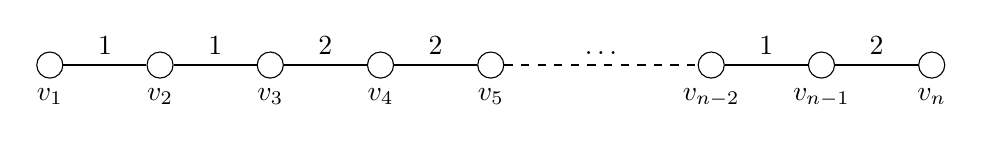
\begin{tikzpicture}
		[scale=.7,auto=left,main node/.style={shape=circle,draw,fill=white}]
		\node [main node] (1) at (1,1) [label=below:$v_1$] {} ;
		\node [main node](2) at (3,1) [label=below:$v_2$] {} ;
		\node [main node](3) at (5,1) [label=below:$v_3$] {} ;
		\node [main node](4) at (7,1) [label=below:$v_4$] {} ;
		\node [main node](5) at (9,1) [label=below:$v_5$] {} ;
		
		\node [main node](6) at (13,1) [label=below:$v_{n-2}$] {} ;
		\node [main node](7) at (15,1) [label=below:$v_{n-1}$] {} ;
		\node [main node](8) at (17,1) [label=below:$v_n$]  {};
		
		
		\path[draw,thick]
		(1) edge node {1} (2)
		(2) edge  node {1} (3)
		(3) edge  node {2} (4)
		(4) edge  node {2} (5)
		
		(5) edge [dashed]  node {$\ldots$} (6)
		
		(6) edge  node {1} (7)
		(7) edge  node {2} (8)
		;
		
		\end{tikzpicture}
		\caption{Primer utežitve grafa $P_n$.}
	\label{pn}
	\end{figure}
	Res, zgornja utežitev zadošča zgornjemu pogoju. Na sliki ~\ref{pn} vidimo primer take utežitvne na grafu $P_n$. Glede na to, da sta zadnji uteži na povezavah $1$ in $2$ lahko sklepamo, da gre na sliki za $P_n$ z $n \equiv 3 \pmod{4}$. Prav tako opazimo, da je pravzaprav pomembno zaporednje uteži $11221\ldots 112$. V tem zaporedju se torej nujno razlikujeta elementa na razdalji 2. Tako lahko zaključimo, da je $\ec(P_n) = 2$ za $n \ge 4$. 

Premislimo sedaj še to kako bi izračunali iregularnostno moč za $P_n$. Zgornja utežitev seveda ne deluje saj nam inducira le štiri različne barve kar pomeni, da ima veliko vozlišč enako barvo. Zato bomo tukaj postopali malenkost drugače. Utežitev bomo poizkušali konstruirati na tak način, da bodo barve vozlišč zavzele vse vrednosti od $1$ do $n$. Recimo, da je $n$ liho. Dodelimo vozlišču, ki se nahaja na sredini (torej z indeksom $\lfloor \frac{n}{2} \rfloor + 1$) barvo z vrednostjo $n$. Sedaj povezavama, ki sta incidenčni sredinskemu vozlišču dodelimo uteži $\lfloor \frac{n}{2} \rfloor$ in $\lceil \frac{n}{2} \rceil$. Nadaljujemo z dodeljevanjem novih uteži, tako da bodo imela vozlišča levo od sredinskega vozlišča sodo vrednost in desno od sredinskega vozlišča liho vrednost. Malo bolj pazljivi mormo sicer biti na posameznih koncih poti, da se naše uteževanje uspešno zaključi. Na podlagi tega torej sklepamo, $\s(P_n) \ge \lceil \frac{n}{2} \rceil$ in je potem zgoraj zastavljena tudi precej stroga.
\end{proof}
Naravno nadaljujemo z grafom, ki ga iz poti dobimo, tako da združimo krajšiča poti z novo povezavo. Tedaj seveda ustvarimo cikel $C_n$. Kljub temu, da grafu dodamo le eno novo povezavo, pri tem strogo povečamo parameter $\ec.$
\begin{trditev}[Domneva 1-2-3 za cikle $C_n$]
Naj bo $C_n$ cikel. Tedaj velja $\ec(C_n) \le 3.$
\end{trditev}
\begin{proof}
	
	V prejšnjem primeru smo izračunali število $\ec$ za $P_n$. Hitro opazimo, da med potjo in ciklom ni veliko razlike. Dodana je le ena povezava med prvim in zadnjim vozliščem. Enako kot v prejšnjem primeru bomo oštevilčili povezave cikla $C_n$ kot $e_1, e_2, \ldots, e_n$, kjer vzamemo $e_n = v_n v_1$. Poizkusimo z enako utežitvijo kot smo jo imeli za poti, torej
		\begin{equation*}
	\omega(e_i) = \begin{cases}
			1, &\text{če } i \equiv 1,2 \pmod{4} ;\\ 
			2, &\text{če } i \equiv 3,4 \pmod{4} .
	\end{cases}
	\end{equation*}
	
\begin{figure}[]
	\centering 
	\begin{subfigure}{0.475\textwidth}
		\centering 
		\begin{tikzpicture}
	
		[scale=.8,auto=left,main node/.style={draw=none,fill=none}]
		\def \n {7}
		\node[
		regular polygon,
		regular polygon sides=\n,
		minimum size=4cm,
		rotate=180/\n,
		] (a) {};
		
		\node[draw=none,fill=none] (1) at (a.corner 1) [] { $v_1$};
		\node[draw=none,fill=none] (2) at (a.corner 2) [] { $v_2$};
		\node[draw=none,fill=none] (3) at (a.corner 3) [] { $v_3$};
		
		\node[draw=none,fill=none] (4) at (a.corner 5) [] { $v_{n-2}$};
		\node[draw=none,fill=none] (5) at (a.corner 6) [] { $v_{n-1}$};
		\node[draw=none,fill=none] (6) at (a.corner 7) [] { $v_n$};
		
		\draw[] (1) to node [above left] {1}  (2);
		\draw[] (2) to node [left] {1}  (3);
		\draw[bend right, dashed] (3) to node [] {}  (4);
		\draw[] (4) to node [ right] {1}  (5);
		\draw[] (5) to node [above right] {2}  (6);
	
		\draw[] (6) to node [above] {2}  (1);
		\end{tikzpicture}
		\caption{Primer $n = 4k$. Zadoščata 2 uteži}
	\end{subfigure}
	\hfill
	\begin{subfigure}{0.475\textwidth}
		\centering 
		\begin{tikzpicture}
		[scale=.6,auto=left,main node/.style={draw=none,fill=none}]
		\def \n {7}
		\node[
		regular polygon,
		regular polygon sides=\n,
		minimum size=4cm,
		rotate=180/\n,
		] (a) {};
		
		\node[main node] (1) at (a.corner 1) [] { $v_1$};
		\node[main node] (2) at (a.corner 2) [] { $v_2$};
		\node[main node] (3) at (a.corner 3) [] {\ $v_3$};
		
		\node[main node] (4) at (a.corner 5) [] { $v_{n-2}$};
		\node[main node] (5) at (a.corner 6) [] { $v_{n-1}$};
		\node[main node] (6) at (a.corner 7) [] { $v_n$};
		
		\draw[] (1) to node [above left] {1}  (2);
		\draw[] (2) to node [left] {1}  (3);
		\draw[bend right, dashed] (3) to node [] {}  (4);
		\draw[] (4) to node [ right] {2}  (5);
		\draw[] (5) to node [above right] {2}  (6);
		\
		\draw[] (6) to node [text=red,above] {3}  (1);
		\end{tikzpicture}
		\caption{Primer $n = 4k + 1$. Potrebno je dodati utež $3$ na zadnjo povezavo.}
	\end{subfigure}
	\vskip\baselineskip
		\begin{subfigure}{0.475\textwidth}
			\centering 
		\begin{tikzpicture}
		[scale=.6,auto=left,main node/.style={draw=none,fill=none}]
		\def \n {7}
		\node[
		regular polygon,
		regular polygon sides=\n,
		minimum size=4cm,
		rotate=180/\n,
		] (a) {};
		
		\node[main node] (1) at (a.corner 1) [] { $v_1$};
		\node[main node] (2) at (a.corner 2) [] { $v_2$};
		\node[main node] (3) at (a.corner 3) [] {\ $v_3$};
		
		\node[main node] (4) at (a.corner 5) [] { $v_{n-2}$};
		\node[main node] (5) at (a.corner 6) [] { $v_{n-1}$};
		\node[main node] (6) at (a.corner 7) [] { $v_n$};
		
		\draw[] (1) to node [above left] {1}  (2);
		\draw[] (2) to node [left] {1}  (3);
		\draw[bend right, dashed] (3) to node [] {}  (4);
		\draw[] (4) to node [ right] {2}  (5);
		\draw[] (5) to node [above right] {1}  (6);
	
		\draw[] (6) to node [text=red,above] {3}  (1);
		\end{tikzpicture}
		\caption{Primer $n = 4k + 2$.}
	\end{subfigure}
	\hfill
	\begin{subfigure}{0.475\textwidth}
		\centering 
		\begin{tikzpicture}
		[scale=.6,auto=left,main node/.style={draw=none,fill=none}]
		\def \n {7}
		\node[
		regular polygon,
		regular polygon sides=\n,
		minimum size=4cm,
		rotate=180/\n,
		] (a) {};
		
		\node[main node] (1) at (a.corner 1) [] { $v_1$};
		\node[main node] (2) at (a.corner 2) [] { $v_2$};
		\node[main node] (3) at (a.corner 3) [] {\ $v_3$};
		
		\node[main node] (4) at (a.corner 5) [] { $v_{n-2}$};
		\node[main node] (5) at (a.corner 6) [] { $v_{n-1}$};
		\node[main node] (6) at (a.corner 7) [] { $v_n$};
		
		\draw[] (1) to node [above left] {1}  (2);
		\draw[] (2) to node [left] {1}  (3);
		\draw[bend right, dashed] (3) to node [] {}  (4);
		\draw[] (4) to node [ right] {1}  (5);
		\draw[] (5) to node [text=red,above right] {3}  (6);

		\draw[] (6) to node [text=red,above] {$\{2,3\}$}  (1);
		\end{tikzpicture}
		\caption{Primer $n = 4k + 3$. Poleg zadnje povezave moramo popraviti še predzadnjo.}
	\end{subfigure}
\caption{Primer utežitve cikla $C_n$ glede na različne vrednosti $n$. Uteži, obarvano rdeče so potrebni popravki popravki utežitve $\omega$, da dobimo pravilno barvanje cikla.}
\label{fig:cnall}
\end{figure}
Potreben in zadosten pogoj, ki smo ga uporabili že za primer poti velja tudi za cikle. Pri ciklu moramo opazovati dodatno povezavo med $v_1$ in $v_n$. Kot je razvidno iz slike~\ref{fig:cnall} moramo ločit primere glede na vrednost $n \pmod{4}$. Ugotovimo, da za pravilno utežitev cikla $C_n$ potrebujemo največ 3 uteži, torej $\ec(C_n) \le 3$. Pokažimo sedaj, da je ta meja tudi natančna za $n \neq 4k$. Recimo torej nasprotno, da je $\mu(C_n) = 2$ in naj bo $\omega$ utežitev, ki zadošča temu pogoju. Potem iz $c_{\omega}(v_i) \neq c_{\omega}(v_{i+1})$ sledi $\omega(v_i v_{i+1}) \neq \omega({v_{i+2} v_{i+3}})$. To je pogoj, da se uteži na razdalji $2$ razlikujejo. Ampak to pomeni, ker imamo na voljo samo uteži 1 in 2, da mora veljati $\omega(v_i v_{i+1}) = \omega({v_{i+4} v_{i+5}})$. To pa je protislovje v primeru ko $n \neq 4k$.

Nahitro ocenimo še parameter $s(C_n)$. V tem primeru par tako vzamemo idejo, ki smo jo dobili pri uteževanju poti. Zopet začnemo nekje na sredini in v tem primeru poizkušamo dosečti, da se uteži na vozliščih nahajajo na intervalu $[2, n+1]$. Podobno koti pri poti je potrebno biti pazljiv pri robnih primerih vendar zagotovo velja enaka ocena in sicer $\s(G) \ge \lceil \frac{n}{2} \rceil$.
	
	
\end{proof}
Do sedaj smo obravnavali grafe z precej nizkimi stopnjami vozlišč. Na podlagi tega bi lahko sklepali, da je v tem primeru enostavno računati parameter $\ec$, saj je malo možnih konflikov med vozlišči. Vendar poleg manjšega števila sosedov imajo vozlišča seveda tudi manjše število incidenčnih povezav in s tem manj svobode kakšne vrednosti lahko zasedejo. Sedaj si bomo ogledali iskanje primerne utežitve na polnih grafih $K_n$. 
\begin{trditev}[Domneva 1-2-3 za $K_n$~\citet{examples} ]
\end{trditev}
Naj bo $K_n$ polni graf na vsaj treh vozliščih. Tedaj velja $\ec(K_n) = 3$.
	\begin{proof}


Poglejmo najprej zakaj velja $\ec(K_n) \ge 3$. Recimo, da to ne drži. Torej imamo neko $2$-utežitev $\omega$ za $K_n$ iz česar sledi, da je $c_{\omega}(v_i) \neq c_{\omega}(v_j)$ za vsak $ i \neq j$. To pomeni, da mora vsak $c_{\omega}(v_i)$ za $i=1,2,\ldots,n$ pripadati eni izmed $n$ različnih vrednosti v $\{n-1, n, \ldots, 2(n-1)\}$. Tako lahko najdemo vozlišče $v'$ za katerega $c_{\omega}(v') = n-1$ in vozlišče $u'$ za katerega $c_{\omega}(u') = 2(n-1)$, to pa je protislovje saj $\omega(v'u') = 1$ zaradi vozlišča $v'$ in $\omega(v'u') = 2$ zaradi $u'$.

 Pozkusimo sedaj najti $3$-utežitev $\omega$, ki je pravilno barvanje z utežmi. Sedaj imamo za $c_{\omega}(v_i)$ na voljo eno izmed $3n$ vrednosti izmed $\{n-1, n, \ldots, 3(n-1)\}$. Skonstruirali bomo utežitev $\omega$ na naslednji način. Najprej oštevilčimo vozlišča kot $v_1, v_2, \ldots, v_n$. V prvem koraku nastavimo vse uteži na 1. Uteži z vrednostjo 2 in 3 dodelimo povezavam, tako da dobimo strogo naraščajoče zaporedje $\left(c_{\omega}(v_i)\right)_{i \in [n]}$. Označimo še $N_j = \{n, n-1, \ldots, n - j + 1\} \setminus \{v_j\}$ in nastavimo
 \begin{equation*}
 \begin{split}
 \omega(v_1 v_n) &= 2 \text{ za } i \in N_1 \\
 \omega(v_2v_i) &=2 \text{ za } i \in N_2\\
 \vdots \\
 \omega(v_jv_i) &= 2 \text{ za } i \in N_j .
 \end{split}
 \end{equation*}
Sedaj velja 

$$ c_{\omega}(v_i) = \underbrace{n-1}_{\text{Uteži z vr. 1}} + \underbrace{|N_i|}_{\text{Uteži z vr. 2}}   = n-1 + 
\begin{cases}
 i, & \text{če } i\notin N_i \iff i < n - i +1; \\
  i - 1, & \text{če } i \in N_i \iff i \ge n - i + 1.
\end{cases} $$
Iz zgornje enačbe vidimo, da zaporedje strogo narašča do največjega $i$, za katerega $ i < n - i +1$ to pa je natanko tedaj ko $ i =  \lfloor \frac{n}{2}\rfloor$. Takrat velja
$$|N_{i}|  =| N_{i+1}| \implies c_{\omega}(v_i) = c_{\omega}(v_{i+1}).$$
Te enakosti se znebimo, tako da dodamo uteži $\omega(v_iv_n) = 3$ za $\lfloor \frac{n}{2}\rfloor < i < n$ in dobimo
$$c_{\omega}(v_i) =
\begin{cases}
n + 1 + i, & \text{če } i < n; \\
\lfloor \frac{5n-5}{2}\rfloor, & \text{če }i=n.
\end{cases} .
 $$
 To pa je pravilno barvanje $K_n$ in zato $\ec(K_n) = 3$.

Ker je graf poln mora seveda vsako vozlišče imeti svojo barvo. To pomeni, da v primeru polnih grafov velja $\s(K_n) = \ec(K_n) = 3$.
 

\end{proof}
 
 \subsection{Dvodelni in $3$-obarljivi grafi}
V prejšnjem razdelku smo obravnavali grafe, ki imajo podobno strukturo. Sedaj se bomo osredotočili na grafe, z nizkim kromatičnim številom. Najnižje možno kromatično število je $2$ zato bomo najprej obravnavali dvodelne grafe. Medtem ko bomo domnevo dokazali za splošne dvodelne grafe bomo v nekaterih posebnih primerih to mejo še izboljšali.

 
 Dvodelne grafe označimo kot $G=(A, B, E)$, kjer sta $A$ in $B$ biparticija vozlišč.
Obravnavajmo najprej polne dvodelne grafe $K_{m,n}$ z biparticijo $(A, B)$. Enostavni primer je, ko velja $m \neq n$. V tem primeru lahko vse povezave utežimo z 1 in dobimo pravilno barvanje, kar pomeni $\ec(K_{m,n}) = 1$. V kolikor je $m=n$ oštevilčimo vozlišča v $A$ kot $v_1, v_2, \ldots, v_m$ in vozlišča v $B$ kot $u_1, u_2, \ldots, u_n$. Sedaj definiramo utežitev kot
$$
\omega(v_i u_j) = 
\begin{cases}
1 , &\text {če } (i, j) \in [m-1] \times [n]; \\
2, & \text{če } i=m; j \in [n].
\end{cases}.
$$
Zgornja utežitev poskrbi, da imajo vozlišča $u_i$ vrednost $c_{\omega}(u_i) = m + 1$ vozlišča $v_i$ pa $c_{\omega}(v_i) = m$ z izjemo $c_{\omega}(v_m) = 2n$. To je torej pravilno barvanje in $\ec(K_{m,n}) = 2$. Sedaj bomo obravnavali še nekaj bolj splošnih dvodelnih grafov.


\begin{trditev}[~\citet{examples}]
\label{dvosodo}	
Naj bo $G =(A,B,E)$ dvodelen graf. V kolikor je $|A|$ ali $|B|$ sodo, potem $\ec(G) \le 2$.
\end{trditev}
\begin{proof}
Brez škode za splošnost bomo predpostavili $|A|$ sodo. Trditev bomo dokazali, tako da bomo skonstruirali $2$-utežitev $\omega$ za katero bo veljalo, da je $c_{\omega}(u)$ sodo za $u \in A$ in liho za $u \in B$. S tem bo trditev dokazana. Označimo vozlišča v množici $A$ kot $a_1, a_2, \ldots, a_{2r}$ in naj bo $P_i$ pot od $a_i$ do $a_{i + r}$. Take poti obstajajo za vsak $i = 1, 2, \ldots, r$ saj je graf povezan. Utežitev $\omega$ konstruiramo, tako da začnemo z $\omega(e) = 0$ za vsako povezavo $e$. Vsakič ko neka pot $P_i$ vsebuje povezavo $e$ utež na tej povezavi povečamo za 1. Barvanje $c_{\omega}$, ki ga inducira utežitev $\omega$ ima naslednjo lastnost:
\begin{itemize}
\item $c_{\omega}(u) = 1 \pmod{2}$ za $u \in A$
\item $c_{\omega}(u) = 0 \pmod{2}$ za $u \in B$.
\end{itemize}
To izhaja iz dejstava, da se vsaka pot $P_i$ začne in konča v množici $A$ in s tem za vsako vozlišče $u \in B$, ki se nahaja na poti, poveča vrednost $c_{\omega}(u)$ za $2$. Seveda enako velja za vmesna vozlišča $u \in A$ medtem ko začetnemu in končnemu vozlišču poveča vrednost barvanja le za 1. Ker smo poti $P_i$ definirali na tak način, da je vsako vozlišče v $A$ natanko enkrat začetek ali konec neke poti sledi zgornja lastnost. Sedaj uteži na povezavah zreduciramo $\pmod{2}$ kar še vedno ohranja zgornjo lastnost. Tako dobljena utežitev še vedno inducira pravilno barvanje in uporablja uteži z vrednostmi  v $\{0,1\}$. Preprosto spremenimo uteži z vrednostjo $0$ v $2$ in dobimo ustrezno $2$-utežitev grafa $G$.
\end{proof}

\begin{posledica}[~\citet{examples}]
Za dvodelen graf $G = (A, B, E)$ z $\delta(G)=1$ velja $\ec(G)  \le 2$.
\end{posledica}
\begin{proof}
Po zgornji trditvi lahko predpostavimo, da sta tako $|A|$ in $|B|$ lihi. Brez škode za splošnost predpostavimo, da $d(x) = 1$ za nek $x \in A$. Ker je graf povezan obstaja povezava $xy \in E$ do nekega vozlišča $y \in B$. Dodatno velja, da je $d(y) > 1$, saj je graf povezan. Potem za graf $G - x$ velja, da je povezan dvodelen graf  za katerega je $|A -  \{x\}|$ sodo. Po prejšnji trditvi za ta graf obstaja $2$-utežitev $\omega'$, ki inducira pravilno barvanje. Sedaj utežimo povezavo $xy$ z 2 in dobimo ustrezno utežitev $\omega$, saj velja $c_{\omega}(x) = 2$ in $c_{\omega}(y) > 2$ ter še vedno sodo.
\end{proof}
Kot smo že omenili so vsa drevesa dvodelni grafi, kjer imajo vsi listi stopnjo ena. Na podlagi tega dejstva sledi naslednja posledica.
\begin{posledica}
Za drevo $T$ z vsaj tremi vozlišči velja $\ec(T) \le 2$.
\end{posledica}
Zgornja posledica izhaja iz dejstva, da ima vsako drevo vsaj 1 list ter posledično vozlišče s stopnjo 1. Sedaj si bomo ogledali še eno trditev, ki nam bo omogočala izračuna $\ec(G)$ za dvodelne regularne grafe.
\begin{izrek}[~\citet{examples}]
\label{dvoreg}
Naj bo $G = (A,B, E)$ dvodelen graf. V kolikor za vsako povezavo $uv \in E$ velja $\lfloor \frac{d(u)}{2} \rfloor + 1 \neq d(v) $ potem $\ec(G) \le 2$.
\end{izrek}
Preden se lotimo dokaza zgornjega izreka bomo neko pomožno trditev, ki velja za splošne dvodelne povezane grafe.
\begin{trditev}[~\citet{examples}]
\label{t1}
V grafu $G = (A, B, E)$ obstaja vozlišče $x$, tako da so vozlišča $G - N[x]$ v množici $A$ vsa v isti povezani komponenti grafa $G -  N[x]$.
\end{trditev}

\begin{proof}[Dokaz trditve \ref{t1}]
brez škode za splošnst predpostavimo $x \in B$. Izberimo vozlišče $x \in B$, tako da  maksimalna komponenta v $G - N[x]$ postane čim večja ter jo označimo kot $G_1 = (A_1, B_1, E_1)$. Sedaj za protislovje predpostavimo, da ima graf  $G - N[x]$ še eno povezano komponento $G_2 = (A_2, B_2, E_2)$, kjer je množica $A_2$ neprazna. Ker je začeten graf $G$ povezan obstaja povezava med $N(x)$ in $B_1$.  Izberimo si sedaj poljuben $x' \in A_2$ in opazujmo graf $G - N[x']$. Opazimo, da sta $G_1$ in $N[x]$ v isti povezani komponenti katere velikost je strogo večja od velikosti $G_1$, kar pa je v protislovju z izbiro vozlišča $x$.
\end{proof}

\begin{proof}[Dokaz izreka \ref{dvoreg}]
Po trditvi \ref{dvosodo} predpostavimo, da sta tako $|A|$ kot $|B|$ lihi.
Po trditvi \ref{t1} lahko sklepamo, da ima graf $G - N[x]$ komponento $G_1 = (A_1, B_1, E_1)$, kjer je $A_1 = A \setminus N(x)$, vse ostale komponente pa so izolirana vozlišča v $B$. Sedaj obravnavajmo dva primera.

V kolikor je $d(x)$ liho je potem $|A_1|$ sodo. Po trditvi \ref{dvosodo} ima graf $G_1$ $2$-utežitev $\omega'$ z lastnostjo $f_{\omega'}(u)$ je liho za $u \in A_1$ in  $f_{\omega'}(u)$ je sodo za $v \in B_1$. Sedaj $\omega'$ razširimo do $\omega$, tako da utežimo povezave incidenčne $x$ z 1 ter z 2 vse ostale povezave. Za $\omega$ velja $c_{\omega}(u)$ je liho za $u \in A$  in $c_{\omega}(v)$ je sodo za $B \setminus \{x\}$. Prav tako velja $c_{\omega}(x) = d(x)$ in $c_{\omega}(u) = 2d(u) - 1$ za $u \in N(x)$. Po predpostavki izreka tako velja tudi $c_{\omega}(x) \neq c_{\omega}(u)$ za $u \in N(x)$. Tako je $\omega$ $2$-utežitev, ki je pravilno barvanje z utežmi.

V koliko je $d(x)$ sodo je $|A_1|$ liho. Ker je graf $G$ povezan obstaja vozlišče $u^* \in N(x)$, ki je soseden $v^* \in B_1$. Označimo sedaj graf $G'$, kot graf, ki ga dobimo iz $G_1$, tako da dodamo povezavo $u^*v^*$. V tem primeru lahko za $G' = (A_1 \cup \{u^*\}, B_1, E_1 \cup \{u^*v^*\})$ uporabimo trditev \ref{dvosodo}, da dobimo $2$-utežitev $\omega'$ z že znano lastnostjo. Sedaj $\omega'$ razširimo v $\omega$, tako da utežimo povezave incidenčne $x$ razen $xu^*$ z 1 ter vse ostale povezave z 2. Sedaj velja $c_{\omega}(x) = d(x) + 1$ in $c_{\omega}(u) = 2d(u) - 1$ za vse $u \in N(x) \setminus \{u^*\}$. Po predpostavki izreka tako zopet velja $c_{\omega}(x) \neq c_{\omega}(u)$ ter $\omega$ $2$-utežitev, ki je pravilno barvanje z utežmi. S tem je izrek dokazan.
\end{proof}
\begin{posledica}

Za vsak dvodelen $d$-regularen graf $G$ z $d \ge 3$ velja $\ec(G) = 2$. 
\end{posledica}

Za regularne grafe predpostavka izreka \ref{dvoreg} avtomatsko velja, izjema so le $2$-regularni grafi oziroma cikli. Preprost proti primer je $C_6$, ki je dvodelen ter $2$-regularen graf vendar velja $\ec(C_6) = 3$. Zato je pogoj $d \ge 3$ v posledici nujno potreben.

 Kot smo ugotovili lahko nekatere dvodelne grafe utežimo le z utežema $1$ in $2$ vendar to ne velja za vse dvodelne grafe. Naravno naslednje sledijo $3$-obarljivi grafi. 
  V članku ~\citet{base}  sta  avtorja zastavila vprašanje, ki je nato pripeljalo do domneve 1-2-3 in ga v njem tudi dokazala za primer $3$-obarljivih grafov. Glavna ideja, zakaj domneva velja za 3-obarljive grafe je v tem, da v tem primeru uteži lahko gledamo po modulu 3. To je res, saj v primeru ko imamo neko utežitev z poljubnimi utežmi, ki inducira pravilno 3-barvanje lahko vse uteži reduciramo po modulu 3 in še vedno ohranimo pravilno 3-barvanje. Izrek, ki ga bomo dokazali v tem delu bo malenkost močnejši. Pri tem bo ena izmed njegovih posledic dokaz domneve 1-2-3 v primeru 3-obarljivih grafov. Za množico uteži bomo dovolili poljubno Abelovo grupo $\Gamma$. V ta namen bomo dokazali nekaj lastnosti Abelovih grup, ki jih bomo kasneje uporabili v dokazu glavnega izreka.
  \begin{trditev}
  	Naj bo $\Gamma$ Abelova grupa z $|\Gamma| = n$ in naj $0$ označuje enoto. Tedaj za vsak $g \in \Gamma$ velja $n g = 0$.
  \end{trditev}

\begin{proof}
	Vzemimo poljuben $g \in \Gamma$ in definirajmo preslikavo $f_g : \Gamma \rightarrow \Gamma$ kot
	$$f_g(h) = g + h .$$
	Ta preslikava je bijekcija saj je $f_{-g}$ njen inverz. Iz tega sklepamo, da je $ g + \Gamma = \Gamma$ za vsak $g$. Sedaj vidimo, da $ \sum_{h \in \Gamma} h = \sum_{h \in \Gamma} (g + h) = ng + \sum_{h \in \Gamma} h$. Iz tega sledi $ng = 0$.
\end{proof}


\begin{trditev}
	Naj bo sedaj $\Gamma$ Abelova grupa lihe moči in $|\Gamma| = n$. Tedaj za vsak element $g \in \Gamma$ obstaja $h \in \Gamma$, tako da $g = 2h$.
\end{trditev}

\begin{proof}
	Ker je $\Gamma$ Abelova grupa po prejšnji trditvi vemo, da $ 0 = ng$. Prištejemo $g$ na obeh straneh in dobimo $g = (n+1)g$. Sedaj označimo $h = \frac{n + 1}{2}g$ in očitno velja $g = 2h$.
\end{proof}

Podobno ne velja za Abelove grupe sode moči. To preprosto vidimo na primeru ciklične grupe $\mathbb{Z}_4 = \{0,1,2,3\}$, kjer elementa $3$ ne moremo zapisat na tak način.


  \begin{izrek}[~\citet{base}]
  	Naj bo $\Gamma$ Abelova grupa lihe moči in G ne-trivialen $|\Gamma|$-barljiv graf. Potem obstaja utežitev $\omega$ z elementi iz $\Gamma$, tako da je inducirano barvanje $c_{\omega}$ pravilno.
  \end{izrek}

\begin{proof}
	Označimo $\Gamma = \{g_1, g_2, \ldots, g_k\}$. Naj bo $c$ neko barvanje grafa $G$ z največ $k$ barvami in označimo z $n_i \le 0$ število vozlišč barve $i$ za $1 \le i \le k$. Po zadnji trditvi vemo, da obstaja $h \in \Gamma$, tako da $n_1g_1 + n_2g_2 + \ldots n_kg_k = 2h$. Sedaj na poljubno povezavo grafa dodamo utež $h$. Na vse preostale povezave damo utež $0$. Tako je vsota vseh uteži na vozliščih enaka $2h$. V nadaljevanju bomo spremenili utežitev, tako da ohranjamo skupno utežitev vozlišč konstantno ( = $2h$), dokler vsa vozlišča barve $i$ nimajo uteži $g_i$. Recimo torej, da obstaja vozlišče $u$ barve $i$, ki ima napačno utež $g$ in velja $g \neq g_i$. Ker je vsota uteži na vozliščih ves čas konstantna in $n_1g_1 + n_2g_2 + \ldots n_kg_k = 2h$ obstaja vsaj še eno drugo vozlišče $v$ z napačno utežitvijo. Sedaj najprej obravnavajmo primer, ko $G$ ni dvodelen graf. V tem primeru lahko najdemo sprehod lihe dolžine med $u$ in $v$. Potujemo po sprehodu od $u$ do $v$ in utežem na povezavah zaporedoma prištevamo $g_i - g, g - g_i, \ldots, g_i - g$, tako kot na sliki \ref{im1} . Tak popravem utežitve ohranja skupno utežitev vozlišč ter spremeni le uteži za $u$ in $v$. Po končanem postopku ima vozlišče $u$ sedaj utež $g_i$ kar je željen rezultat. Ta postopek ponavljamo, dokler nimajo vsa vozlišča pravilne utežitve. Sprehod lihe dolžine je nujno potreben, če želimo ohraniti skupno utežitev vozlišč.
 \begin{figure}[h!]
\caption{Popravljanje utežitve z liho potjo.}
\label{im1}
\centering
    \includegraphics[scale=0.5]{3col.png}
    \end{figure}
	
	Oglejmo si sedaj še primer, ko je graf $G$ dvodelen. V primeru nedvodelnega grafa smo vsakemu vozlišču barve $i$ dodelili utež $g_i$. Kljub temu, da je dvodelne grafe lahko pobarvamo z dvema barvama le tega ne moremo vedno storiti z utežitvijo povezav z elementi $\Gamma$. To bi pomenilo $n_1 g_1 = n_2 g_2$, kjer $n_1 g_1$ predstavlja skupno utež vozlišč ene barve in $n_2 g_2$ skupno utež druge barve. Seveda mora enakost držati, saj vsaka povezava pripomore isti delež tako prvi kot drugi vsoti. Ta enačba pa ni vedno rešljiva za $g_1 \neq g_2$. Zato v tem primeru postopamo malo drugače. Ker je graf dvodelen, lahko zapišemo njegovo množico vozlišč kot $V(G) = A \cup B$, kjer sta $A$ in $B$ biparticija. Sedaj si izberemo vozlišče $x \in A$, ki ima stopnjo vsaj 2. Zaradi predpostavke lahko to vedno naredimo. Sedaj izberemo $g_1 = 2h$ in $g_1 \neq g_2 = 0$ ter na vse povezave damo utež 0 oziroma $g_2$. Sedaj na enak način popravljamo utežitev, tako da ohranjamo skupno utež 0 (oz. $g2$). V tem primeru smo že dosegli, da imajo vsa vozlišča iz $B$ utež 0. Popraviti moramo torej le uteži za vozlišča v množici $A$. To storimo, tako da za vsako vozlišče $u \neq x \in A$, ki ima utež 0 najdemo pot sode dolžine od $u$ do $x$. Na poti popravljamo povezave, tako da jim priševamo uteži $g_1 - g_2, g_2 - g_1, \ldots, g_2 - g_1$. S tem poskrbimo, da je vozlišče $u$ pravilno uteženo. Ko končamo postopek imajo vsa vozlišča v $A$ utež $g_1$ razen vozlišče $x$, ki ima utež $g = -(n_1 - 1) g_1 = (1 - n_1) g_1$. V kolikor $(1 - n_1)g_1 \neq 0$ smo končali saj smo konstruirali pravilno barvanje. V nasprotnem primeru na dve poljubni povezavi incidenčni $x$ dodamo utež $h$. S tem poskrbimo, da imajo vsa vozlišča v $A$ utež $g_1$, vozlišča v $B$ pa uteži $g_2 = 0$ in $h$.
\end{proof}

Iz zgornjega izreka torej sledi, da domneva velja za $3$-obraljive grafe. Preprosto za take grafe uporabimo ciklično grupo $\mathbb{Z}_3 = \{0,1,2\}$. Nato vse uteži z vrednostjo $0$ zamenjamo z utežjo $3$. S tem še vedno ohranimo pravilno barvanje. Iz utežitve povezav smo na naraven način prišli do barvanja na grafu. Vprašanje je bilo potem ali je to barvanje pravilno. Zgornji izrek pove nekako obratno. Torej, če imamo neko $k$-barvanje in je $k$ liho število potem lahko eksplicitno konstruiramo utežitev z $k$ elementi, ki porodi tako barvanje.


 


V tem razdelku smo izračunali parameter $\ec(G)$ za nekaj posebnih družin grafov ter za grafe z nekaj dodatnimi pogoji. V vseh primerih smo 1-2-3 domnevo potrdili v posebnih primerih smo lahko zgornjo mejo še celo malo izboljšali. Rezultate tega razdelka lahko predstavimo s spodnjo tabelo.
\begin{table}[H]

\caption{\label{tab:tab1} Izračun $\ec(G)$ za znane grafe. }
\centering
\begin{tabular}{|l|l|}
\hline
 Graf $G$ & $\ec(G)$  \\ \hline
 $P_n$ & 2  \\ \hline
 $C_n$ & $\begin{cases}
	2 ,& \text{če } n = 4k;\\ 
	3 & sicer;
	\end{cases}$  \\ \hline
 $K_n$& 3  \\ \hline
 $K_{m,n}$& $\begin{cases}
	1 ,& \text{če } nm \neq n\\ 
	2 & sicer;
	\end{cases}$  \\ \hline
 3 obarljivi& 3  \\ \hline
$T_n$ & 2  \\ \hline
dvodelni in $d$ -regularni z $d \ge 3 $ & 2  \\ \hline
\end{tabular}
\end{table}

\subsection{Konstrukcija grafov G z nizkim parametrom $\ec(G)$}

Spoznali smo že kar nekaj grafov z nizko vrednostjo parametra $\ec$. Z nizko vrednostjo imamo v mislih seveda čim nižjo zgornjo mejo. Sedaj si bomo ogledali kako lahko neko ``dobro'' utežitev razširimo na večji graf. V ta namen najprej ponovimo definicijo kartezičnega produkta dveh grafov. Naj bosta $G =(V, E)$ in $G' = (V', E')$ grafa.  \textbf{Kartezični produkt} grafov $G$ in $G'$ je graf, ki ga označimo z $G \Box G'$. Množica vozlišč grafa  $G \Box G'$ je enaka kartezičnemu produktu $V(G) \times V(G')$ iz česar tudi sledi ime za ta produkt. Dve vozlišči $(u, u')$ in $(v, v')$ sta sosednji v $G \Box G'$ natanko tedaj ko $u=v$ in $u'v' \in E(G')$, ali $u' = v'$ in $uv \in E(G)$. Vozlišče $(u, u')$ v kartezičnem produktu ima po zgornji definiciji toliko incidenčnih povezav kot jih ima $u$ v grafu $G$ plus toliko kot $u'$ v grafu $G'$. Velja torej formula $d_{G \Box G'}((u, u')) = d_G(u) + d_{G'}(u')$.
\begin{trditev}
Za vsaka grafa $G$ in $H$ velja $\ec(G \Box H) \le \max \{\ec(g), \ec(H)\}$.
\end{trditev}
\begin{proof}
Trditev bomo dokazali, tako da bomo konstruirali utežitev kartezičnega produkta  $G \Box H$. Naj bo $k =\max \{\ec(g), \ec(H)\} $. Tedaj obstajata utežitvi $\omega_1 : E(G) \rightarrow \{1, \ldots, k\}$ in $\omega_2 : E(H)\rightarrow \{1, \ldots, k\}$, ki porodita pravilno barvanje za grafa $G$ in $H$. Sedaj sestavimo utežitev $\omega : E(G \Box H) \rightarrow \{1, \ldots, k\}$, tako da definiramo 
\begin{equation*}
\omega((u, u'), (v, v')) = \begin{cases}
	\omega_1(uv) ,& \text{če } u' = v';\\ 
	\omega_2(u'v'), &\text{če } u = v.
	\end{cases}
\end{equation*}
Poglejmo sedaj kakšno barvanje porodi zgornja utežitev. Podobno kot pri stopnjah vozlišč v kartezičnem produktu grafov velja $c_{\omega}((u, u')) = c_{\omega_1}(u) + c_{\omega_2}(u')$. Pokazati moramo, da imata vozlišči na vsaki povezavi kartezičnega produkta različne barve. Ampak povezava v kartezičnem produktu obstaja le ko se vozliči ujemata vsaj na eni koordinati. V kolikor se ujemata na prvi koordinati trditev sledi ker $\omega_2$ inducira pravilno barvanje v kolikor pa se ujemata na drugi koordinati trditev sledi ker $\omega_1$ inducira pravilno barvanje.
\end{proof}
Na podlagi zgornje trditve lahko, iz grafov za katere smo domnevo 1-2-3 že dokazali, konstruiramo nove grafe za katere domneva tudi velja. Oglejmo si nekaj primerov.
\begin{primer}
\textbf{Hiperkocka} je graf $Q_n$ z $2^n$ vozlišči dobljen kot kartezični produkt $n$ kopij grafov $K_2$. Na sliki \ref{hip} vidimo nekaj začetnih hiperkock.
 \begin{figure}[h!]
\caption{Hiperkocke $Q_n$ za $n=1,2,3$.}
\label{hip}
\centering
    \includegraphics[scale=0.4]{car_ex_1.png}
    \end{figure}
Primer $Q_1 = K_2$ izpustimo saj v tem primeru rešitev ne obstaja. Za ostale primere iz slike \ref{hip}  ročno preverimo $\ec(Q_2) = \ec(Q_3) \le 2.$ Nato za vsak $n > 3$ zapišemo hiperkocko kot
 $$Q_n = Q_{\lfloor n/2 \rfloor} \Box Q_{\lceil n/2 \rceil}.$$
 To lahko naredimo saj je operacija kartezičnega produkta asociativna. Ker $n > 3$ je tako dimenzija obeh hiperkock na desni strani zgornje enakosti vsaj $2$. Z uporabo indukcije nato dokažemo $\ec(Q_n) = 2$ za $ n \ge 2$. Izračuna $\ec(Q_n)$ bi se lahko lotili tudi na drug način in sicer z orodjem, ki smo ga do sedaj že uporabili. Namreč za hiperkocko velja, da je dvodelen graf.To lahko pokažemo na več načinov.  Eden izmed njih je indukcija na $n$, kjer zapišemo $Q_n = Q_{n-1} \Box K_2$ ter induktivno uporabimo $2$-barvanje $Q_{n-1}$. V kartezičnem produktu za posamezni kopiji $Q_{n-1}$ uporabimo ravno obratno barvanje. Poleg tega je hiperkocka $Q_n$ tudi $(n)$-regularen graf, kar zopet lahko preverimo z indukcijo. Sedaj lahko uporabimo posledico izreka ~\ref{dvoreg} in direktno dobimo $\ec(Q_n) = 2$.

Na podoben način lahko generiramo tudi t.i.\ torus grafe. \textbf{Torus graf} označimo z $T_{m,n} = C_m \Box C_n$. Direktna posledica zgornje trditve je torej $\ec(T_{m,n}) \le 3$ v kolikor $n,m \ge 3$. Torus graf $T_{m,n}$ si lahko predstavljamo kot $m \times n$ mrežo kjer povežemo sosednje točke ter prav tako povežemo levi in desni rob ter zgornji in spodnji rob. Tako dobimo $4$-regularen graf z $mn$ vozlišči. Vendar na tak način ne moremo dobiti vseh $4$-regularnih grafov na $mn$ vozliščih, saj tak graf ni enolično določen.
\end{primer}




 
 \section{Izrek 1-2-3-4-5}
Do sedaj smo domnevo 1-2-3 potrdili za grafe s posebnimi lastnostmi. Pri iskanju oziroma konstrukciji ustrezne utežitve grafa so ključno vlogo igrale prav te posebne lastnostni.  Kot smo že omenili je bilo od leta 2004 ko je bila zastavljena domneva veliko poizkusov iskanja zgornje meje za parameter $\ec(G)$. V tem kratkem času je bilo narejeno veliko napredka. Različni avtorji so predstavili različne metode in pristope k problemu. Do danes so najboljšo zgornjo mejo predstavili~\citet{proof12345}. Presenetljivo je dokaz sorazmerno preprost in algoritmične narave. V tem razdelku bomo to zgornjo mejo dokazali in analizirali časovno zahtevnost algoritma, ki najde ustrezno utežitev. Dobljen rezultat lahko formuliramo kot naslednji izrek.

 
 \begin{izrek}[Izrek 1-2-3-4-5; ~\citet{proof12345}]
\label{theorem12345}
 	Za vsak enostaven graf $G$, ki ni $K_2$ velja $\ec(G) \le 5$.
 \end{izrek}

\begin{proof}
	Ker je graf povezan in ima vsaj 3 vozlišča vsebuje vsaj eno vozlišče s stopnjo $\ge 2$. Sedaj uredimo vozlišča kot $V(G) = \{ v_1, v_2, \ldots, v_n\}$, tako da je $d(v_n) \ge 2$ in ima vozlišče $v_i$ soseda v množici $\{v_{i+1}, v_{i+2}, \ldots, v_n\}$ za vsak $i \le n-1$. Tako ureditev vozlišč lahko najdemo na preprost način. V vozlišču $v_n$ začnemo BFS algoritem ter v seznam zaporedoma dodajano obiskana vozlišča. Tako dobimo vozlišča urejena kot $\{v_n, v_{n-1}, \ldots, v_1\}$. Za vsak $i \le n-1$ sedaj res velja, da ima soseda v množici   $\{v_{i+1}, v_{i+2}, \ldots, v_n\}$, saj se v tej množici nahaja njegov starš v BFS drevesu.

V nadaljevanju dokaza bomo konstruirali $5$-utežitev $\omega$, ki bo pravilno obarvala graf $G$. Začnemo z začetno utežitvijo $\omega(e) = 3$ za vsako povezavo $e$. Vozlišča bomo procesirali v zgornjem vrstnem redu in pri tem vsako utež modificirali največ dvakrat. Za vsak $i < n$ $v_i$ bomo vozlišču $v_i$ dodeli množico dveh barv $C(v_i) = \{c(v_i), c(v_i) + 2\}$. Dodatno zahtevamo, da velja $c(v_i) \in \{0,1\}  \mod 4$. Ti dve barvi bosta dve izmed možnih končnih barv za vozlišče $v_i$. Ker želimo, da se končna barva razlikuje od končnih barv sosedov zahtevamo, da je presek množic sosednjih vozlišč prazen. To lahko zapišemo bolj natančno, tako da za vsako \textit{povezavo nazaj} $v_jv_i \in E(G)$ z $j < i$ velja $C(v_j) \cap C(v_i) =\emptyset$. Poleg tega bomo utežitev $\omega$ konstruirali, tako da bo veljalo $c_{\omega}(v_i) \in C(v_i)$. Skupaj to torej pomeni, da med prvimi $n-1$ vozlišči ni nobenega konflikta. V zadnjem koraku bomo popravili uteži na povezavah, ki so incidenčne $v_n$, tako da bo $c_{\omega}(v_n)$ različen od njegovih sosedov. S tem bo izrek dokazan.

Začnimo z dodeljevanjem množic barv za vozlišča $C(v_i)$. Začnemo z vozliščem $v_1$, kjer trenutno velja $c_{\omega}(v_1) = 3d(v_1)$ in izberemo $C(v_1)$, tako da $c_{\omega}(v_1) \in C(v_1)$. To lahko naredimo, ker trenutno še nimamo nobenih posebnih omejitev. Sedaj nadaljujemo induktivno. Naj bo $ 2 \le k \le n-1$ in predpostavimo, da smo izbrali $C(v_i)$ za vse $i < k$ ter velja:
\begin{itemize}
\item $c_{\omega}(v_i) \in C(v_i)$ za vse $ i < k$,
\item $\omega(v_kv_j) = 3$ za vse povezave z $ j > k$,
\item če $\omega(v_iv_k) \neq 3$ za neko povezavo z $i < k$ potem $\omega(v_iv_k) = 2$ in $c_{\omega}(v_i) = c(v_i)$ ali $\omega(v_iv_k)=4$ in $c_{\omega}(v_i) = c(v_i) + 2$.
\end{itemize}
Sedaj moramo določiti uteži, tako da bo enako veljalo tudi za volzišče $v_k$. Oglejmo si poljubno povezavo \textit{nazaj} $v_iv_k \in E$ za nek $i < k$. Na podlagi zgornjih pogojev lahko uteži na tej povezavi bodisi prištejemo bodisi odštejemo 2 ter še vedno ohranjamo pogoj $c_{\omega}(v_i) \in C(v_i)$. Recimo, da ima $v_k$ $d$ takšnih sosedov. Potem imamo $d+1$ možnosti za $c_{\omega}(v_k)$, ki so vse iste parnosti (odvisno od parnosti $d$). Vse različne možnosti dobimo, tako da najprej na vseh povezavah \textit{nazaj} nastavimo najnižjo možno utež. S tem dobimo najnižjo možno vrednost $a$ za $c_{\omega}(v_k)$. Sedaj na vsaki povezavi \textit{nazaj} postopoma povečamo utež za $2$. Tako dobimo možnosti $a, a+2, \ldots, a +2d$. Dodatno bomo dovoljevali spremembo za $1$ na prvi povezavi \textit{naprej}. To je povezava \ $v_kv_j \in E$, kjer je $j$ najmanjši tak indeks, da obstaja povezava $v_kv_j$. S tem lahko $c_{\omega}(v_k)$ zavzame vse vrednosti na intervalu $[a-1, a + 2d + 1]$. Različnih vrednosti je torej $2d + 3$. Uteži sedaj modificiramo, tako da bo veljalo

\begin{enumerate}
\item \label{th15:1} $c_{\omega}(v_i) \in C(v_i)$ za vse $ i \le k$,
\item \label{th15:2} $c(v_i) \neq c(v_k)$ za $v_iv_k \in E$, kjer $i < k$,
\item \label{th15:3} bodisi $c_{\omega}(v_k) = c(v_k)$ in $\omega(v_kv_j) \in \{2,3\}$ ali $c_{\omega}(v_k) = c(v_k) + 2$ in $\omega(v_kv_j) \in \{3,4\}$.
\end{enumerate}
Pri tem je pogoj ~\ref{th15:1} vedno izpolnjen. V primeru, ko $c_{\omega}(v_i) = c(v_i)$ lahko uteži na povezavi $v_iv_k$ prištejemo 2. V nasprotnem primeru ko je $c_{\omega}(v_i) = c(v_i) + 2$ lahko uteži na zgornji povezavi odštejemo 2. Pogoj ~\ref{th15:2} nam lahko blokira največ $2d$ vrednosti in pogoj ~\ref{th15:3} kvačjemu blokira krajišči intervala. Tako ostane vsaj ena vrednost za $c_{\omega}(v_k)$. Na tak način lahko konstruiramo množice $W(v_k)$ z želenimi lastnostmi za vse $k < n$.

V zadnjem koraku moramo najti primerno vrednost za $c_{\omega}(v_n)$. V tem primeru nimamo na voljo povezave naprej, ki nam je v prejšnjem primeru pomagala pri določitvi uteži, vendar nam v tem primeru ni potrebno skrbeti za kasnejša vozlišča. Na povezavah $v_iv_n$ za $i < n$ lahko ponovno utež bodisi povečamo bodisi zmanjšamo za 2 in ohranimo $c_{\omega}(v_i) \in C(v_i)$. To nam ponovno da $d(v_n) + 1 \ge 3$ možnosti za $c_{\omega}(v_n)$. V kolikor za najmanjšo izmed teh možnosti $a$ velja $a \in \{2,3\} \mod 4$ potem na vseh povezavah incidenčnih $v_n$ izberemo najnižjo možno utež. S tem bomo poskrbeli, da $c_{\omega}(v_i) = c(v_i) \in \{0,1\} \mod 4$ za $v_i \in N(v_n)$ in tako različna od $a$. V kolikor $a \in \{0,1\} \mod 4$ in obstaja $v_i \in N(v_n)$ z $c(v_i) \neq a$ potem izberemo višjo utež na povezavi $v_iv_n$ in nižjo utež na vseh ostalih povezavah s čimer dobimo $c_{\omega}(v_n) = a + 2$ kar je tudi pravilno barvanje. Nazadnje v kolikor $a \in \{0, 1\} \mod 4$ in $c(v_i) = a$ za vse $v_i \in N(v_n)$ izberemo višjo utež na vsaj dveh povezavah (kar lahko sotrimo, saj je $d(v_n) \ge 2$) in dobimo pravilno barvanje.
\end{proof}

Na podlagi zgornjega dokaza lahko napišemo algoritem za iskanje takih utežitev za poljuben graf. Poleg tega, da nam dokaz zagotavlja rešitev za vsak graf je algoritem, ki tako rešitev poišče polinomske časovne zahtevnosti. To res drži, saj moramo za vsako vozlišče pregledati le vse njegove sosede. Ker lahko število sosedov omejimo z $n$, celoten postopek deluje v časovni zahtevnosti $\mathcal{O}(n^2)$.

\subsection{Izrek 1-2-3-4 za d-regularne grafe}

V prejšnjem razdelku smo analizirali rezultat za splošne grafe. Kot smo že omenili je to tudi najboljši rezultat do danes, ki ga poznamo za splošne grafe. Prav tako smo opazili, da za nekatere posebne grafe lahko rezultat izboljšamo. Ta razdelek bo namenjen $d$-regularnim grafom. Ugotovili smo že, da za regularne grafe $G$, ki so tudi dvodelni velja $\ec(G) \le 2$. Na podlagi motivacije za domnevo 1-2-3 smo po drugi strani ugotovili, da so morda regularni grafi težki za ta problem saj so zelo ``oddaljeni''  od pojma iregularni graf. Kljub temu vseeno lahko izkoristimo nekatere lastnosti regularnih grafov in izboljšamo rezultat iz prejšnjega razdelka. Ta razdelek v veliki meri sledi članku ~\cite{regular}.

\begin{izrek}[Izrek 1-2-3-4 za regularne grafe; ~\citet{regular}]
Za vsak $d$-regularen graf $G$ velja $\ec(G) \le 4$
\end{izrek}

\begin{proof}
V dokazu bomo uporabili podobno metodo kot pri dokazu izreka ~\ref{theorem12345}. Izberimo si sedaj neko poljubno maksimalno neodvisno množico $ I \subseteq V(G)$. To je taka množica vozlišč kjer ne obstaja niti ena povezava med njenimi elementi ter je izmed vseh možnih takih množic največja po kardinalnosti. Na podlagi množice $I$ definiramo še:
\begin{itemize}
\item $R = V \setminus I$,
\item $R_1 \subseteq R$ množica izoliranih vozlišč v $G[R]$,
\item $R_2 = R \setminus R_1$,
\item $G_1, G_2, \ldots G_p$ označujejo povezane komponente v $G[R_2]$.
\end{itemize}
Konstruirali bomo utežitev $\omega$ za katero bo na koncu veljalo:
\begin{enumerate}
\item \label{itm:1} $c_{\omega}(v) < 3d $ za vsak $v \in R_2$
\item \label{itm:2}$c_{\omega}(v) \ge 3d $ za vsak $v \in I$
\item \label{itm:3}$c_{\omega}(v) < 4d $ za vsak $v \in I$, ki ima soseda v $R_1$
\item \label{itm:4}$c_{\omega}(v) \in \{3d - 1, 4d\} $ za vsak $v \in R_1$
\end{enumerate}
Glede na to, da je $I$ neodvisna množica, $R_1$ neodvisna množica v $G[R]$ in ni povezav med $R_1$ in $R_2$ v $G$ na podlagi zgornjih omejitev možni konflikti obstajajo med sosednjimi vozlišči v $R_2$. Zato bomo na to posebno pazili pri konstrukciji utežitve. Za utežitev bomo dodatno zahtevali še:
\begin{itemize}
\item $\omega(e) \in \{1,2,3\}$ za $e \in E(R_2)$
\item $\omega(e) \in \{3,4\}$ za $e \in E(I, R_2)$
\item $\omega(e) \in \{2,3,4\}$ za $e \in E(I, R_1)$
\end{itemize}
Preden določimo začetne uteži si bolj podrobno oglejmo strukturo komponent v $R_2$. V vsaki izmed komponent $G_i$ bomo uredili vozlišča  $v_1, v_2, \ldots, v_n$ na enak način kot pri izreku ~\ref{theorem12345}. Torej veljati mora, da ima vsko vozlišče $v_i$ z $i < n$ \textit{soseda naprej}, kar pomeni, da ima soseda $v_k$ z $ k > i$. To lahko storimo na enak način s pomočjo BFS algoritma. Dodatno mora vsako vozlišče $v \in R_2$ imeti vsaj enega soseda v $I$. V nasprotnem primeru bi sicer $v$ lahko premaknili v $I$ in tkao dobili večjo neodvisno množico, kar je v protislovju z našo predpostavko. To povezavo bomo imenovali \textit{oporna povezava}.

Začetno utežitev definiramo kot

$$ \omega(e) =\begin{cases}
	1 ,&\text{če je $e$ prva povezava naprej za neko vozlišče v } R_2;\\ 
	2, &  \text{če je $e$ povezava v $G[R_2]$, ki ni prva povezava naprej}; \\
	3 ,& \text{če je $e$ incidenčna povezava vozlišču v $I$ in ni oporna povezava}; \\
4, & \text{če je $e$ oporna povezava.} 
	\end{cases}
$$
S to utežitvijo zadoščamo zgornjemu pogoju. Sedaj bomo modificirali uteži na povezavah, tako da bomo odstranimo možne konflikte v $R_2$. Podobno kot v izreku ~\ref{theorem12345} predpostavimo, da trenutno analiziramo komponento $G_i$ ter vozlišče $v_j$. Pri tem smo že analizirali vse prejšnje komponente in vozlišča. Sedaj želimo določiti uteži, tako da bo utež na $v_j$ različna od uteži za $v_1, v_2, \ldots v_{j-1}$. To želimo storiti na tak način, da ne spreminjamo uteži na že analiziranih vozliščih. To bomo izvedli, tako da bomo po potrebi za $1$ spremenili utež na povezavi, ki povezuje $v_j$ z njegovim sosedom nazaj $v_k$ ter njunima opornima povezavama. Bolj natančno recimo, da je $e = v_kv_j$ povezava nazaj in pokažimo, da lahko utež na njej spremenimo za $1$. Označimo še z $e_{v_k}$ oporno povezavo vozlišča $v_k$. Oglejmo si najprej primer, ko $e$ ni prva povezava naprej. Potem velja $\omega(e) = 2$ in $\omega(e_{v_k}) \in \{3, 4\}$. V kolikor je $\omega(e_{v_k}) = 3$ utež na povezavi $e$ zmanjšamo za $1$ na oporni povezavi pa povečamo za $1$. V drugem primeru ko je $\omega(e_{v_k}) = 4$ storimo ravno obratno. Če je $e$ prva povezava naprej za $v_k$ potem uteži na $e$ in $e_{v_k}$ še nista bili spremenjeni in imata začetno vrednost $1$ in $4$. Zaporedoma jih lahko spremenimo v $2$ in $3$. Sedaj uporabimo enak razmislek kot pri prejšnjem izreku. Recimo, da ima vozlišče $v_j$ $d$ povezav nazaj in vsako izmed teh povezav lahko spremenimo za $1$. To nam da $d + 1$ možnih vrednosti za $c_{\omega}(v_j)$ in torej lahko izberemo še nezasedeno vrednost, glede na predhodnja vozlišča.

Z zgornjim postopkom smo zagotovili, da ni konfliktov med vozlišči znotraj $R_2$. Sedaj moramo pokazati, da je postopek spreminjanja uteži v skladen z pogoji~\ref{itm:1},~\ref{itm:2} in~\ref{itm:3}. Opazujmo neko vozlišče $v \in I$. Povezave incidenčne vozlišču $v$ imajo začetno utežitev v množici $\{3,4\}$. Po zgornjem postopku lahko utež na povezavi incidenčni $v$ spremenimo samo v primeru, ko je oprona povezava. Ampak vse oporne povezave smo na začetku utežili z $4$ in jih v postopku kvečjemu zmanjšamo za $1$. To pomeni, da so uteži na povezavah incidenčnih $v$ še vedno v množici $\{3,4\}$. Iz tega sledi pogoj~\ref{itm:2}. V kolikor ima $v$ nekega soseda v $R_1$, je bila začetna utežitev na tej povezavi enaka $3$ in ni bila spremenjena v zgornjem postopku. Zato torej velja tudi pogoj~\ref{itm:3}. Pokažimo, da velja tudi pogoj~\ref{itm:1}. Opazimo najprej, da utež na vsaki povezavi $e$ grafa $G[R_2]$ spremenimo največ enkrat in sicer takrat, ko analizirano vozlišče z enim izmed njegovih sosedov nazaj. Za vsako vozlišče $v \in R_2$, ki ni zadnje vozlišče neke komponente velja, da ima njegova prva povezava naprej utež $1$. Dodatno imajo vse ostale povezave, ki so incidenčne $v$, utež največ $3$. Edina izjema je oporna povezava $e_v$, ki ima utež 4. Iz tega sledi, da $c_{\omega}(v) \le 3d - 1$ ter se ne spreminja ko analiziramo kasnejša vozlišča. Sedaj pokažimo, da enako velja tudi v primeru ko je $v$ zadnje vozlišče neke komponente v $G[R_2]$. To preprosto sledi iz dejstva, da zadnja vozlišča nimajo opornih povezav, kar pomeni da imajo vse povezave incidenčne $v$ utež manjšo ali enako $3$. Poleg tega je povezava $uv$, kjer je $u$ predzadnje vozlišče v zgornji ureditvi prva povezava naprej vozlišča $u$ in je po že uporabljenem premisleku utežena z največ $2$. Iz tega torej sledi pogoj~\ref{itm:1}.
Sedaj smo odpravili konflikte v $R_2$ in poskrbeli, da so uteži še vedno konsistentne z začetnimi zahtevami. To nam zagotavlja, da je $c_{\omega}(v) \neq c_{\omega}(u)$ za vsako povezavo $uv \in E(I \cap R_2)$. Poskrbimo sedaj še za možne konflikte med $I$ in $R_1$, tako da bo veljal pogoj~\ref{itm:4}. Ker je vozlišče $v \in R_1$ incidenčno le z vozlišči v $I$ so vse povezave incidenčne $v$ utežene z $3$. Sedaj za vsako vozlišče $v \in R_1$ postopamo na naslednji način. V kolikor je $c_{\omega}(u') \ge 3d + 1$ za nekega soseda $u'$ vozlišča $v$, spremenimo utež iz $3$ na $2$ na natanko eni izmed povezav. V nasprotnem primeru, ko je $c_{\omega}(u) = 3d$ za vsako vozlišče $u \in N(v)$ spremenimo utež  iz $3$ na $4$ na vsaki povezavi $uv$. Na tak način ohranimo vse pogoje~\ref{itm:1} -~\ref{itm:3} ter, ko obdelamo vsa vozlišča v $R_1$, velja tudi pogoj~\ref{itm:4}. S tem smo našli ustrezno $4$-utežitev.
\end{proof}

Za konec tega razdelka komentirajmo dobljene rezultate. Kot smo že omenili sta oba izreka algoritmične narave in tudi uporabljata podobne ideje. Glavna ideja v obeh primerih je neka začetna utežitev ter nato procesiranje vozlišč v primernem vrstnem redu. Pri tem smo morali biti pazljivi, da ohranjamo določene lastnosti pri že procesiranih vozliščih kar nam omogoča dodatna povezava iz vozlišča, ki ga trenutno procesiramo. Zadnje vozlišče smo v obeh primerih morali obravnavati malo drugače. Oba izreka podajata zelo dobro mejo, ki se precej približa zastavljeni domnevi. Vendar nažalost z podobno idejo težko dosežemo še boljše rezultate. Pri izreku \ref{theorem12345} tako nujno potrebujemo $5$ različnih uteži. Podobno kot pri izreku~\ref{theorem12345} lahko tudi v tem primeru razberemo algoritem, ki bi poiskal ustrezno $4$-utežitev za regularni graf. Vendar v tem primeru ne moremo napisati polinomskega algoritma. Problem je v tem, da moramo poiskati največjo neodvisno množico, ki pa je NP poln problem. Na podlagi tega torej še ne vemo, ali za tak problem obstaja polinomski algoritem. Še več splošno prepričanje je, da tak algoritem ne obstaja. Že iz samega dokaza smo opazli, da je malenkost bolj zahteven kot dokaz izreka ~\ref{theorem12345}. Množico vozlišč grafa smo morali razdeliti v različne množice in obravnavati več primerov. To nam je sicer omogočilo, da smo lahko uporabili eno utež manj.	
 
 \section{Verjetnostne metode}

Rezultati, ki smo jih obravnavali do sedaj so nam eksplicitno podali neko utežitev, ki je zadoščla zahtevanim pogojem. Najboljši rezultat za splošne grafe je izrek \ref{theorem12345}, ki konstruira $5$-utežitev. Ugotovili smo tudi, da lahko v primeru regularnih grafov rezultat v splošnem še malo izboljšamo. V tem razdelku bomo na problem pogledali malenkost drugače. Prav tako bomo poizkušali konstruirati primerno utežitev vendar tokrat ta utežitev morda nebo delovala za vse grafe. V tem primeru bo dovolj, da je rešitev ``dobra'' za večino grafov. Trenutno še ni jasno kaj pomeni izraz ``dobra'' rešitev za večino grafov. To zahtevo si lahko intuitivno predstavljamo na naslednji način. Izberimo si nek $n$ in opazujmo grafe na množici vozlišč $V = \{1,2, \ldots, n\}$. Sedaj nas zanima, ali lahko za poljuben graf na $n$ vozliščih najdemo ``dobro'' utežitev? Na to vprašanje v splošnem še ne moremo odgovoriti, saj se po tem sprašuje tudi domneva 1-2-3. Lahko pa se vprašamo kakšna je verjetnost, da za naključen graf na $n$ vozliščih najdemo ustrezno utežitev. Tekom razdelka bomo definirali pojem ``naključnega grafa'' ter si ogledali nekaj preprostih trditev, ki veljajo za take grafe. Z uporabo preprostih trditev bomo formulirali in dokazali izrek, ki bo za veliko večino grafov podal ustrezno $1$-$2$ utežitev. Pri tem bomo v veliki meri sledili knjigi \citet{maingraph}.

\subsection{Naključni grafi}
Vzemimo ponovno fiksno število $n$ in naj bo $V = \{1,2, \ldots, n\}$ množica $n$ vozlišč. Z oznako $\mathcal{G}$ označimo množico vseh grafov na množici vozlišč $V$.  Ideja je, da množico $\mathcal{G}$ spremenimo v verjetnostni prostor. Nato lahko razmišljamo kakšna je verjetnost, da ima nek $G \in \mathcal{G}$ določeno lastnost. Oziroma kolikšna je pričakovana vrednost neke invariante, recimo kromatično število na grafu $G$.

Intiutivno bomo naključen graf $G$ generirali na naslednji način. Izberemo si $p \in [0, 1]$ in za vsako povezavo $e \in {V \choose 2}$ izvedemo naključen poizkus, ali povezavo vključimo v graf $G$ ali ne. Poizkuse izvajamo neodvisno ter verjetnost uspeha vsakega poizkusa je enaka $p$. Recimo sedaj, da imamo nek fiksen graf $G_0$ na $n$ vozliščih z $m$ povezavami. Kakšna je verjetnost, da naključno generiramo prav ta graf na zgornji način? To je seveda preprost izračun, saj mora poizkus uspeti za vsako izmed $m$ povezav ter spodleteti za mankajoče povezave. Torej verjetnost, da je naključen $G \in \mathcal{G}$ enak grafu $G_0$ je enaka  $p^m (1-p)^{{n \choose 2} - m}$. To je torej verjetnost nekega elementarnega dogodka v verjetnostnem prostoru. Na enak način preprosto izračunamo verjetnosti za vse elementarne dogodke oziroma za vse grafe. Na tem koraku uporabimo nekaj dejstev iz verjetnosti ter teorije mere. Znano je, da v kolikor poznamo verjetnosti za vse elementarne dogodke potem znamo izračunati verjetnost vsakega dogodka. To seveda drži v kolikor je naš verjetnosti prostor končen. V našem primeru to seveda drži, ker je grafov na $n$ vozlišč končno. Pokazati bi bilo še potrebno, da taka verjetnostna mera sploh obstaja, vendar dokaz za naše namene ni zanimiv, bralec ga lahko najde v poglavju 11 v \cite{maingraph}. Označimo še naš verjetnosti prostor kot $\mathcal{G} = \mathcal{G}(n, p)$. Sedaj si bomo ogledali nekaj preprostih izračunov povezanih z naključno generiranimi grafi.

\begin{trditev}
\label{indeprand}
Za vsa naravna števila $n,k$ z $n \ge k \ge 2$ je verjetnost, da ima $G \in \mathcal{G}(n,p)$ največjo neodvisno množico z največ $k$ elementi, enaka
$$ P[\alpha(G) \ge k] \le {n \choose k} q ^{k \choose 2} .$$
\end{trditev}
Pri tem je z oznako $\alpha(G)$ mišljena velikost največje neodvisne množice.
\begin{proof}
Verjetnost, da je neka množica $U \subseteq V$ velikost $k$ neodvisna v $G$ je $q^{k \choose 2}$, saj mora poizkus spodleteti na vsaki možni povezavi med vozlišči iz $U$. Ampak vseh različnih množic $U$ velikosti $k$ je natanko ${n \choose k}$. Za vsako izmed $k$ elementnih podmnožic $U$ seštejemo verjetnosti, da je ta množica neodvisna. Ker so vse te verjetnosti enake dobimo željeno zgornjo mejo in trditev sledi.
\end{proof}

Na podoben način lahko dokažemo ogromno zanimivih lastnosti grafov, vendar jih za naš primer nebomo potrebovali. Kot zanimivost mogoče navedimo dejstvo, da so naključni grafi $G \in \mathcal{G}(n, p)$ močno povezani tudi za majhne vrednosti $p$. To pomeni, da so naključni grafi v splošnem povezani. Pri tem velja omenit še to, da je generacija naključnih grafov zelo preprosta medtem ko je generiranje strogo povezanih grafov težek problem. Na podlagi zgornje ugotovitve lahko simuliramo generiranje povezanih grafov. Enostavno generiramo poljuben naključen graf in preverimo, če je povezan. V kolikor ni povezan postopek ponovimo. Ker je verjetnost, da je naključen graf na $n$ vozliščih nepovezan zelo majhna nam za generiranje povezanih grafov nebo potrebno velikokrat ponavljati generiranja.

Sedaj lahko definiramo to, kar smo se spraševali na začetku razdelka. Naj $\mathcal{P}$ označuje neko invariano oziroma lastnost grafa. Na podlagi tega se lahko vprašamo kako se obnaša verjetnost $P[G \text{ ima lastnost } \mathcal{P}]$ za $G \in \mathcal{G}(n, p)$ ko $n \rightarrow \infty$. V kolikor gre ta verjetnost proti $1$ rečemo, da ima graf $G$ lastnost $\mathcal{P}$ skoraj zagotovo. Oziroma skoraj vsi grafi imajo lastnost $\mathcal{P}$. Naslednja trditev nam bo podajala spodnjo (ter tudi zgornjo) mejo za kromatično število za skoraj vse grafe.
\begin{trditev}
Za vsako konstanto $p \in (0,1)$ in vsak $\epsilon > 0$ ima skoraj vsak graf $G \in \mathcal{G}(n, p)$ kromatično število
$$ \chi(G) > \frac{\log(1/q)}{2 + \epsilon} \cdot \frac{n}{\log n} $$
\end{trditev}
\begin{proof}
Po trditvi \ref{indeprand} za vsak fiksen $n \ge k \ge 2$ sledi:

\begin{equation}
\begin{split}
P[\alpha(G) \ge k]  &\le {n \choose k} q ^{k \choose 2} \\
& \le n^k q ^{k \choose 2} \\
&= q^{k \frac{\log n}{\log q} + \frac{1}{2}k(k-1)} \\
&= q^{\frac{k}{2}\left(- \frac{2 \log n}{\log(1/q)} + k - 1\right)}.
\end{split}
\end{equation}

Kjer vzamemo $k = (2 + \epsilon) \frac{\log n}{\log (1/q)}$. Za tako izbiro gre eksponent proti neskončnosti ko povečujemo $n$, ter celoten izraz gre proti $0$ saj je $q < 1$. Iz tega sklepamo, da je skoraj vsak $G \in \mathcal{G}(n, p)$ tak, da v kateremkoli barvanjo $G$ nima nobenih $k$ vozlišč iste barve, saj bi to pomenilo neodvisno množico velikosti $k$. Iz tega sledi, da vsako barvanje vsebuje več kot 
$$ \frac{n}{k} = \frac{\log (1/q)}{2 + \epsilon} \cdot \frac{n}{\log n} $$
barv.
\end{proof}

Zgornjo trditev bomo kasneje uporabili ko bomo analizirali utežitve na naključnih grafih. V primeru ko $\epsilon$ zamenjamo z $-\epsilon$ gre eksponent v zgornjem dokazu proti $0$ ko povečujemo $n$. Pri gre celoten izraz proti $1$. Na podoben način kot v dokazu zgornje trditve iz tega sledi, da skoraj vsako barvanje vsebuje manj kot $n/k$ barv kar nam podaja zgornjo mejo za kromatično število. Ta zgornja meja je torej $\chi(G) < \frac{\log(1/q)}{2 - \epsilon} \cdot \frac{n}{\log n}$ in jo bomo uporabili pri dokazu glavnega izreka v tem razdelku. Poleg tega bomo potrebovali še eno asimptotsko oceno in sicer za minimalno stopnjo vozlišč. Naj bo $p \in (0, 1)$ in vzemimo graf $G \in  \mathcal{G}(n, p)$ ter opazujmo poljubno vozlišče $v \in V(G)$. Kaj lahko povemo o $d(v)$? Mislimo si lahko, da izvedemo eksperiment za vsakega izmed preostalih $n - 1$ vozlišč ter povečamo stopno vozlišča $v$ v kolikor je bil eksperiment uspešen. Na podlagi tega lahko ocenimo pričakovano stopnjo vozlišča kot $(n-1)p$. Na tem mestu lahko uporabimo Chernoffovo mejo ter ugotovimo, da velja $P[d(v) \le (p - \epsilon)n] \rightarrow 0$ ko pošljemo $n$ v neskončnost. Tako lahko sklepamo, da ima skoraj vsak graf $G \in  \mathcal{G}(n, p)$ naslednjo lastnost

$$ d(G) \ge (p - \epsilon)n .$$

Glavni namen tega razdelka je podati neko asimptotsko oceno za parameter $\ec(G)$ oziroma bolj natančno podali bomo trditev, ki bo pokazala, da skoraj za vse grafe velja $\ec(G) = 2$ kar je zelo preseneltjiv rezultat saj je še boljši kot sama domneva. Da nam bo uspelo pokazati zgornje si moramo ogledati še nek rezultat, ki nima nič opravit z verjetnostnimi metodami ampak z iskanjem posebnih faktorjev v grafu. Nato bomo uporabili vse rezultate iz tega razdelka in formulirali ter dokazali končno trditev.

\subsection{Podgrafi z omejenimi stolpnjami}
Za dokaz glavnega izreka v tem razdelku potrebujemo nek bolj tehničen izrek, ki nam podaja obstoj posebnih vpetih podgrafov. Glavna ideja je v tem, da si za vsako vozlišče izberemo kakšno stopnjo želimo, da ima v vpetem podgrafu. Ugotovili bomo, da za pravilno izbiro stopenj lahko vedno najdemo tak vpet podgraf.


Naj bo $G =(V, E)$ graf in naj bo $H$ njegov vpet podgraf. V kolikor je graf $H$ $k$-regularen rečemo tudi, da je $H$ \textbf{$k$-faktor} grafa $G$.  Iskanje določenih faktorjev v grafu je ekvivalentno nekaterim drugim problemov na grafih. Naprimer $1$-faktor v grafu predstavlja popolno ujemanje. Nas bo v tem razdelku zanimala bolj splošna definicja faktorja.  Recimo, da sta $f$ in $g$ celoštevilski funkciji na množici vozlišč in velja $0 \le g(v) \le f(v) \le d(v)$ za vsako vozlišče $v \in V(G)$. Tako definiramo \textbf{$(g,f)$-faktor} grafa $G$ kot vpet podgraf $H$ z lastnostjo $g(v) \le d_H(v) \le f(v)$ za vsako vozlišče $v$. Želimo si torej, da ima naš vpet podgraf stopnje vozlišč med vnaprej podanima funkcijama. Naslednja trditev nam podaja potreben in zadosten pogoj, ki nam pove kdaj nek graf vsebuje določen $(g, f)$- faktor.

 \begin{trditev}[~\citet{factor}]
Naj bo $G=(V, E)$ graf ter $f$ in $g$ celoštevilski funkciji na množici vozlišč $V$, tako da velja  $0 \le g(v) \le f(v) \le d(v)$ za vsako vozlišče $v \in V(G)$. Če je $G$ dvodelen ali $g(v) \neq f(v)$ za vse $v$, potem obstaja vpet podgraf $H$ grafa $G$, ki je $(g, f)$-fakotr natanko tedaj ko za vsako množico $S \subseteq V(G)$ velja:

$$\sum_{v \not \in S}(g(v) - d_{G-S}(v)) \le f(S) $$
\end{trditev}

Dokaz zgornje trditve je posledica bolj splošnega izreka, lahko pa se jo dokaže tudi neodvisno na malo bolj preprost način. Ker je dokaz sorazmerno zahteven in rahlo nepovazan z temo magisterske naloge ga izpuščamo. Raje bomo s pomočjo zgornje trditve dokazali trditev, ki jo bomo direktno uporabili pri dokazovanju asipmtostkih rezultatov 1-2-3 domneve.

\begin{izrek}[~\citet{random12}]
\label{factor}
Naj bo $G = (V, E)$ graf in za vse $v \in V$ cela števila $a_v^-$, $a_v^+$, tako da $a_v^- \le \lfloor d(v)/2 \rfloor \le a_v^+ < d(v)$ in $a_v^+ \le min \left( \frac{d(v) + a_v^-}{2} + 1, 2a_v^- + 3 \right)$, potem obstaja vpet podgraf $H$ grafa $G$, tako da $d_H(v) \in \{ a_v^-, a_v^- + 1, a_v^+, a_v^+ + 1\}$ za vse $v \in V$.
\end{izrek}

\begin{proof}
Dokaza se bomo lotili z protislovjem zato predpostavimo, da tak podgraf $H$ ne obstaja. Naj bo dana množica celih števil $\{ a_v  || v \in V\}$ in nek podgraf $H$ grafa $G$ ter definiramo \textit{primankljaj} glede na števila $a_v$ kot vrednost
$$D = \sum_v \max(0, a_v - d_H(v)) .$$ 
Izberemo $a_v \in \{a_v^-, a_v^+\}$ in $b_v = a_v +1$, kjer sta $a_v^-$ in $a_v^+$ kot v formulaciji trditve. Sedaj izberemo še vpet podgraf $H \subset G$, tako da za vsak $v \in V$ velja $d_H(v) \le b_v$. Izmed vse takih možnosti izberemo tisto, ki minimizira primankljaj $D$.  Sedaj trdimo, da obstaja vsaj eno vozlišče $v \in V$ za katerega $d_H(v) < a_v$ ter posledično $D > 0$. To je res, saj v nasprotnem primeru  velja $d_H(v) = a_v$ ali $d_H(v) = b_v = a_v + 1$, kar pa pomeni, da je $H$ iskan podgraf.

Dokaz bomo sedaj nadaljevali, tako da bomo na podlagi podgrafa $H$ definirali množici $A$ in $B$, ki bosta v protislovju z  \begin{figure}[h!]
\caption{Primer $H$-alternirajočega spredoda, ki se konča bodisi v $A$, bodisi v $B$.}
\label{im1}
\centering
    \includegraphics[scale=0.5]{alt1.png}
    \end{figure}prejšnjo trditvijo in iz česar bomo lahko sklepali, da je bila naša predpostvka napačna ter mora obstajati iskan podgraf $H$. 
Definirajmo množico $A_0 = \{v : d_H(v) < a_v\}$ in \textit{H-alternirajoč sprehod} kot sprehod $P = v_0v_1\ldots v_k$, ki se začne v vozlišču $v_0 \in A_0$ in dodatno velja $v_iv_{i+1} \in G-H$ za sod $i$ ter $v_iv_{i+1} \in H$ za lih $i$. Tak sprehod se torej začne v nekem vozlišču iz $A_0$ nato nadaljuje do nekega vozlišča preko povezave, ki je ni v $H$, nato po povezavi v $H$ in tako dalje. Sedaj označimo množici
\begin{itemize}
\item $A = \{v \text{ : obstaja $H$-alternirajoč sprehod sode dolžine, ki se konča z $v$}\}$ in
\item $B =\{v \text{ : obstaja $H$-alternirajoč sprehod lihe dolžine, ki se konča z $v$}\}.$
\end{itemize}
Ker število $0$ štejemo kot sodo število velja $A_0 \subseteq A$. Poleg tega za vsak $v \in A$ velja tudi $d_H(v) \le a_v$, saj v nasprotnem primeru obrnemo katere povezave so v $H$ ter $G-H$ tekom sodega alternirajočega sprehoda, ki se konča z $v$ saj s tem povečamo stopnjo $d_H(v_0)$ za ena in s tem zmanjšamo primankljal kar pa je v protislovju saj smo graf $H$ izbrali, tako da je primankljal minimalen. Na podoben način ugotovimo, da za vsak $v \in B$ velja $d_H(v) = b_v$. V nasprotnem primeru zopet zamenjamo povezave tekom lihega alternirajočega sprehoda, ki se konča z $v$. Ker velja $a_v < b_v$ pomeni, da sta množici $A$ in $B$ disjunktni. Naj bo sedaj $v \in A$ in recimo, da obstaja neka povezava $vw \in E$. V kolikor $w \notin B$ potem mora veljati $vw \in H$ saj bi v nasprotnem primeru lahko sprehod, ki se konča z $v$ podaljšali do $w$ in tako dobili lih alternirajoč sprehod kar bi postavilo vozlišče $w$ v množico $B$. Velja tudi obratno, torej če je $v \in B$ ter povezava $vw \in  E$ ter $w \notin A$ potem $vw \notin H$. S pomočjo teh ugotovitev bomo vsoto $\sum_{v \in A} d_H(v)$ prešteli na drugačen način in sicer, tako da bomo posamezno stopnjo vozlišča $d_H(v)$ z $v \in  A$ razdelili na 2 dela. Prvi del bo sestavljen iz sosedov od $v$, ki niso v $B$. Do vseh teh sosedov lahko po ugotovitvi pridemo le po povezavi, ki se nahaja v $H$. Zato velja $d_H(v) > d_{G-B}(v)$ za vsak $v \in A$. Mankajo torej še vsi sosedje $v$, ki se nahajajo v $B$. V ta namen si podrobno oglejmo neko vozlišče $u \in B$. Po ugotovitvi od prej vemo, da so vsi sosedje od $u$, do katerih pridemo po neki povezavi iz $H$ v množici $A$ in to so natanko tiste povezave, ki jih v prvem primeru nismo prešteli. Vse skupaj lahko torej zapišemo kot
$$\sum_{v \in A} d_H(v) = \sum_{v \in A} d_{G-B}(v) + \sum_{v \in B} d_H(v). $$
Levo in desno stran še malo dodelamo in dobimo
$$ \sum_{v\in A}a_v > \sum_{v \in A} d_H(v) = \sum_{v \in A} d_{G-B}(v) + \sum_{v \in B} d_H(v) =\sum_{v \in A} d_{G-B}(v) + \sum_{v \in B} b_v . $$
Ko sedaj levo in desno stran spravimo skupaj dobimo
$$ S_A = \sum_{v\in A}a_v - d_{G-B}(v) > \sum_{v \in B} b_v = S_B.$$
Dokaz s protislovjem bomo zaključili, tako da pokažemo še obratno in sicer $S_A \le S_B$. V ta namen bomo uporabili še neuporabljene predpostavke izreka in pokazali serijo preprostih trditev:

\begin{enumerate}
\item \label{fac:1} $\sum_ {v\in A}d_B(v) = \sum_{v \in B}d_A(v)$,
\item \label{fac:2} $\forall v \in A$,  $a_v - d_{G-B}(v) \le d_B(v)/2$ in
\item  \label{fac:3} $\forall v \in B$,  $b_v \ge d_A(v)/2.$

\end{enumerate}
Trditev ~\ref{fac:1} enostavno dokažemo z dvojnim štetjem. Za vsako vozlišče $v \in A$ preštejemo njegove sosede, ki so v $B$. Pri tem lahko nekatera vozlišča sicer štejemo večkrat vendar to ni težava, saj v tem štetju vsako povezavo med $A$ in $B$ štejemo natanko enkrat. Prav tako vse povezave med $A$ in $B$ dobimo, če za vsako vozlišče $v \in B$ preštejemo vse njegove sosede v $A$. Za dokaz trditve ~\ref{fac:2} vzemimo poljuben $v \in A$ in predpostavimo $d_H(v) < a_v$. To lahko storimo za vsako posamezno vozlišče v $A$, saj v nasprotnem primeru, ko velja $d_H(v) = a_v$ zamenjamo povezave, ki so v $H$ tekom alternirajočega sprehoda in s tem ne spremenimo primankljaja $H$ (povečamo za 1 v vozlišču $v$ in zmanjšamo za 1 v začetnem vozlišču sprehoda) prav tako se ne spremenita množici $A$ in $B$. To preprosto vidimo, ker za vozlišče $v$ sedaj velja $v \in A_0$ in je začetno vozlišče sprehodov, tako lihih kot sodih. Sedaj moramo obravnavati dva primera in sicer prvič ko je $a_v = a_v^-$ in drugič ko je $a_v = a_v^+$. V prvem primeru je zadeva preprosta saj $a_v^- \le d(v)/2$ po drugi strani velja $d_{G-H}(v) /2 + d_B(v) \ge d(v)/2$ in trditev velja. Oglejmo si še primer ko $a_v = a_v^+ > d(v)/2$. Predpostavljamo lahko dodatno še $d_ {G-B}(v) > a_v^- + 1$ saj v nasprotnem primeru ko nastavimo $a_v = a_v^-$ in odstranimo nekaj povezav med $v$ in $B$ zmanjšamo primankljaj. Sedaj na podlagi predpostavke o $a_v^+$ velja
$$a_v \le \frac{d(v)}{2} + \frac{a_v^-}{2} + 1 < \frac{d(v)}{2} + \frac{d_{G-B}(v)}{2} + \frac{1}{2} = d_{G-B}(v) + \frac{d_B(v)}{2} + \frac{1}{2}, $$
ter ker je $a_v$ celo število in je bil $v \in A$ poljuben trditev ~\ref{fac:2} drži. Pokazati torej moramo še trditev ~\ref{fac:3}. Vzemimo poljuben $v \in B$ in predpostavimo, da $a_v = a_v^- < \lfloor d(v)/2 \rfloor$ saj v drugem primeru avtomatsko velja $b_v \ge d(v)/2 \ge d_A(v)/2$. Predpostavimo sedaj, da trditev ne drži torej $2b_v < d_A(v)$ oziroma $d_A(v) \ge 2a_v + 2 + 1$ in s tem tudi $d_A(v) \ge a_v^+$ zaradi predpostavke izreka. Ker velja $b_v = d_H(v)$ in, ker smo ugotovili, če gre neka povezava, ki je v $H$ iz vozlišča $v \in B$ potem mora drugo vozlišče nujno biti v množici $A$, je natanko $d_A(v) - b_v$ povezav med $v$ in množico $A$, ki niso v $H$. Bolj natančno obstaja neko vozlišče $w \in N(v) \cap A$, tako da $uw \notin H$. Kot smo pokazali zgoraj, lahko zagotovimo, da $d_H(w) < a_w$ ter s tem ne spremenimo dejstva, da je $vw \in H$. Ko nastavimo $a_v = a_v^+$ in dodamo $a_v^+ - d_H(v)$ povezav od $v$ do $A$ v $H$ ter s tem tudi povezavo $vw$ znižamo primankljaj in s tem dokažemo trditev ~\ref{fac:3} ter izrek. To preprosto vidimo saj s pomočjo zgornjih trditev velja
$$ S_A =  \sum_{v\in A}a_v - d_{G-B}(v) \le \sum_{v \in A} d_B(v)/2 = \sum_{v \in B} d_A(v) /2 \le \sum_{v \in B} b_v = S_B,$$
kar je seveda protislovje saj smo malo prej pokazali $S_A > S_B$.
 \end{proof}

Zgornji izrek oziroma dokaz je bil kar težak ter ne ravno najbolj povezan z temo magisterske naloge ampak nam bo omogočal dokazati zanimivo asimptotsko lastnost 1-2-3 domneve, ki smo jo omeneli že malo prej. Poleg tega so ~\citet{random12} uporabili zgornji izrek, da so dokzali $\ec(G) \le 16$ za poljuben graf. Takrat je to bil tudi najboljši rezultat za splošne grafe. Poleg uporabe zgornjega izreka so konstruirali želeno utežitev na precej zahteven način, medtem ko opazimo, da je izrek ~\ref{theorem12345} zares preprost v primerjavi z prejšnjimi poizkusu kljub temu, da podaja precej boljši rezultat.

Podajmo še hiter premislek zakaj nas bi zanimalo iskanje posebnih vpetih podgrafov oziroma kako nam lahko pomagajo pri reševanju 1-2-3 domneve. Predstavljajmo si, da lahko najdemo vpet podgraf $H \subset G$ za katerega velja $d_H(v) \neq d_H(w)$ za vsako povezavo $vw \in E(G)$. Potem lahko utežimo povezave v $H$ z $1$ vse ostale z $0$ in dobimo vozliščno barvanje z uteženimi povezavami z utežmi v $\{0,1\}$. Vendar tak podgraf $H$ v splošnem ne obstaja in seveda smo tak primer že videli saj preprost graf $C_3 = K_3$ ne premore takega podgrafa. Vendar vseeno lahko s pomočjo te ideje dokažemo naslednji izrek.

\begin{izrek}[Asimptotsko obnašanje $\ec(G)$; ~\citet{random12}]
Naj bo $G$ naključen graf izbran iz $\mathcal{G}(n,p)$ za konstanten $p \in (0,1)$. Potem asimptotično skoraj zagotovo velja $\ec(G) = 2$. Natančneje obstaja $2$-povezavna utežitev, tako da so uteži/barve sosednjih vozlišč različne $\mod 2 \chi(G)$.
\end{izrek}

\begin{proof}
Naj bo $G \in \mathcal{G}(n,p)$. Fiksiramo $\epsilon > 0$. Tekom razdelka smo pokazali, da asimptotično skoraj zagotovo veljata naslednji dve dejstvi:
\begin{itemize}
\item $\min_v d(v) > (p- \epsilon)n$,

\item $\chi(G) < \frac{\log(1/(1-p))}{2 - \epsilon} \cdot \frac{ n}{\log n}.$
\end{itemize}
Ker sta števili $p$ in $\epsilon$ fiksirani lahko preprosto izpeljemo, da velja asimptotično skoraj zagotovo velja $ \chi(G) < \min_vd(v) / 6$ za dovolj velik $n$. Predpostavili bomo, da ta neenakost velja in konstruirali $2$-utežitev, ki bo tudi pravilno barvanje grafa $G$.

Naj bo $\{ V_1, V_2, \ldots, V_{\chi(G)}\}$ particija množice vozlišč v neodvisne množice. Sedaj za vsak $v \in V_i$ izberemo $a_v^- \in [ \lfloor d(v)/3 \rfloor,\lfloor d(v)/2 \rfloor]$ in $a_v^+ \in [ \lfloor d(v)/2 \rfloor,\lfloor 2d(v)/3 \rfloor]$, tako da $a_v^- + d(v) \equiv a_v^+  d(v) \equiv 2i \mod 2\chi(G)$. Take izbire obstajajo saj intervala $ [ \lfloor d(v)/3 \rfloor,\lfloor d(v)/2 \rfloor]$ in $ [ \lfloor d(v)/2 \rfloor,\lfloor 2d(v)/3 \rfloor]$ vsebujeta vsaj $2\chi(G)$ zaporednih celih števil. Pri tem je seveda pomembno tudi, da $i \le \chi(G)$. Poleg tega taka izbira za $a_v^-$ in $a_v^+$ zadoščata predpostavkam izreka \ref{factor}, tako da obstaja vpet podgraf $H \subseteq G$ kjer za vsak $v$ velja $d_H(v) \in \{a_v^-,a_v^+,a_v^- + 1 ,a_v^+ + 1\}$.Sedaj konstuiramo utežitev $\omega$ kot 

$$ \omega(e) = \begin{cases}
	1 & e \in E(G) - E(H)\\ 
	2 & e \in E(H) 
	\end{cases} .$$
Izračunajmo sedaj utež na nekek vozlišču $v \in V_i$

$$ \sum_{e \ni v} \omega(e) = 2 d_H(v) + d_{G-H}(v) = d_{G}(v) + d_H(v) \in \{2i, 2i + 1\} \pmod{2\chi(G)}.$$
S tem smo pokazali, da imajo sosednja vozlišča v različnih barvnih razredih $V_i$ različne parnosti in tako konstruirana utežitev porodi pravilno barvanje.
\end{proof}

Za konec tega razdelka bomo komentirali dobljene rezultate. Definirali smo verjetnostni prostor naključnih grafov, kjer smo naključne grafe generirali, tako da smo za vsako povezavo izvedli \textit{enak poizkus} neodvisno od prejšnjih in z enako verjetnostjo uspeha. S pomočjo tega smo za nekaj grafovskih invariant ocenili kako se obnašajo pri naključnih grafih ter si ogledali njihovo asimptotsko obnašanje. Poleg verjetnostnih metod smo dokazali izrek, ki nam pod določenimi pogoji garantira obstoj posebnega vpetega podgrafa, ki ima omejene stopnje vozlišč. Ta izrek sicer nima nič skupnega z verjetnostnimi metodami, ampak nam je omogočal določiti asimptotsko oceno za parameter $\ec(G)$. Presenetljivo smo pokazali, da velja $\ec(G) = 2$ za skoraj vse grafe kar je še boljše kot pravi 1-2-3 domneva. Presenetljivo je tudi zato, ker smo v začetnem delu dokazali, da za nekatere grafe velja $\ec(G) = 3$. Taki so naprimer že nekateri cikli, polni grafi ter nekateri izmed dvodelnih grafov. Iz vidika našega zadnjega rezultata si to lahko predstavljamo tako, da so zgoraj našteti grafi za katere velja $\ec(G) = 3$ redki v verjetnostnem prostoru naključnih grafov. To torej pomeni, da če naključno izberemo nek graf potem skoraj zagotovo to nebo polni graf, cikel ali dvodelni graf z $\ec(G) = 3$. Kljub temu, da je asimptotski rezultat pozitiven iz vidika 1-2-3 domneve nam pri dokazovanju domneve ne koristi prav preveč. Problem je v tem, da še vedno obstaja neskončno število grafov za katere lahko velja $\ec(G) > 2$ in z naivnim pristopom ne moremo poiskati vseh takih grafov.

Zgornji rezultat ni edini rezultat v okviru 1-2-3 domneve, ki uporablja verjetnostne metode. Vendar se v magisterski nalogi nebomo neposredno okvarjali z tem pristopom ampak vseeno bomo uporabili močno orodje, ki izhaja iz verjetnostnih metod.

\section{Polna verzija}
V tem razdelku se bomo posvetili izpeljani verziji 1-2-3 domneve. Do sedaj smo povezavam grafa dodelili uteži ter nato opazovali dobljene uteži na vozliščih kot vsoto uteži na incidenčnih povezavah. Na enak način bomo definirali \textbf{polno utežitev} grafa, kjer bomo poleg povezavam uteži dodelili tudi vsakemu vozlišču. Dobljena polna utež na vozlišč bo tako vsota uteži na incidinčnih povezavah ter uteži na samem vozlišču. V izogib nejasnostim bomo utežitev, ki smo jo obravnavali v prejšjih razdelkih rekli povezavna utežitev. Poleg tega bomo uporabljali izraz polna utež vozlišča za vsoto uteži na povezavah in vozlišču. Z drugimi besedami gre za barvo vozlišča, ki jo porodi polna utežtev.

\begin{definicija}
\textbf{Polna $k$-utežitev} grafa $G=(V,E)$ je preslikava

$$ \omega : E(G) \cup V(G) \rightarrow [k]. $$
\end{definicija}
Na podlagi zgornje utežitve lahko definiramo še \textbf{polno utež} vozlišča $v \in V(G)$ kot

$$c_{\omega}^t(v)  = \omega(v) +  \sum_{u \in N(v)} \omega(vu).$$
Sedaj se seveda lahko sprašujemo enaka oziroma podobna vprašanja kot pri povezavni utežitvi grafa. Za nas najbolj zanimivo vprašanje je ali obstaja kakšna zgornja meja za $k$, tako da je inducirano barvanje grafa tudi pravilno. Označimo z $\ect(G)$ najmanjši tak $k$ za katerega obstaja polna $k$-utežitev grafa, ki inducira pravilno barvanje. Hitro ugotovimo, da je ta problem malo lažji kot pri povezavni utežitvi saj velja

$$ \ec \le \ect. $$
To preprosto dejstvo opazimo, če imamo neko povezavno utežitev, ki je tudi pravilno barvanje potem vozlišča utežimo z konstantno utežjo $1$ in dobimo polno utežitev, ki je tudi pravilno barvanje. Zato nas zanima, ali lahko rezultate, ki smo jih dosegli za parameter $\ec$ izboljšamo in poiščemo nižjo mejo za parameter $\ect$.

Za začetek si bomo ogledali nekaj preprostih primerov na podoben način kot smo to storili pri parameteru $\ec$. Pred tem pa formulirajmo še domnevo, ki se nanaša na parameter $\ect$.
\begin{domneva} 
	\label{12conjecture}
	Naj bo $G$ povezan graf, ki ni $K_2$. Tedaj je $\ect(G) \le 2.$ 
\end{domneva}
Domneva torej pove, da v kolikor dovoljujemo še uteži na vozliščih potem v glavnem potrebujemo eno utež manj, da dobimo pravilno barvanje. Hitro najdemo primer, zakaj v splošnem velja $\ect(G) > 1$. Tak primer je recimo $C_3$ oziroma $K_3$.
\begin{trditev}
$\ect \le 2$ za dvodelne grafe.
\end{trditev}
\begin{proof}
Dokaz trditve je precej preprost in lažji kot v primeru povezavne utežitvije. Naj bo $G = (A,B, E)$ dvodelni graf. Povezavam  poljubno dodelimo uteži $1$ in $2$ medtem ko vozliščem dodelimo uteži, tako da bodo polne uteži vozlišč v množici $A$ sode in lihe v množici $B$. Preprosto, če ima vozlišče $v \in A$ že sodo utež mu dodelimo $2$ in se mu parnost ne spremeni. V nasprotnem primeru mu dodelimo utež $1$ in mu s tem spremenimo parnost. Enako naredimo za vozlišča v množici $B$.
\end{proof}
Zgornja trditev torej dokaže 1-2 domnevo za poti $P_n$ ter drevesa $T_n$. Oglejmo si še naslednjo trditev.
\begin{trditev}
$\ect \le 2$ za cikle $C_n$.
\end{trditev}
\begin{proof}
Postopamo zelo podobno kot smo na začetku dokazali $\ec(C_n) \le 3$. Oštevilčimo vozlišča kot $v_1, v_2, \ldots, v_n$ ter povezave kot $e_i = v_iv_{i+1}$. Sedaj utežitev $\omega$ definiramo na enak način kot v prvem primeru in sicer kot
\begin{equation*}
	\omega(e_i) = \begin{cases}
	1 &i \equiv 1,2 \pmod{4}\\ 
	2 &i \equiv 3,4 \pmod{4}
	\end{cases}
	\end{equation*}
V primeru parametra $\ec$ smo morali obravnavali 4 različne možnosti in sicer glede na $ n \pmod{4}$. Zelo podobno bomo naredili tudi sedaj, vendar potencialnih konflikotv nebomo reševali z tem, da neko povezavo utežimo z $3$ ampak bomo z $2$ utežili nekaj vozlišč. Ta postopek je bolj preprost zato ga bomo samo skicirali. Vsa vozlišča začetno utežmo z $1$. Recimo, da pride do nekega konflikta med dvema vozliščema v ciklu. Izberemo si enega izmed teh vozlišč ter mu dodelimo utež $2$ s čimer smo rešili originalen konflikt, vendar smo pri tem lahko ustvarili novega. Nadaljujemo z istim postopkom, kjer pazimo, da se ne zaciklamo, tako da vozliščem dodeluje utež $2$ vedno v isti smeri. Naprimer izberemo si smer urinega kazalca. Na tak način, bomo morali utež vozlišču popraviti največ trikrat, saj bomo slej ko prej prišli do vozlišča, ki bo imel na obeh povezavah utež $2$ prav tako pa bo tudi sam nosil utež $2$ in bo s tem imel skupno utež $6$. Vendar take uteži nima nobeno ostalo vozlišče zato se zgornji postopek konča po največ treh korakih.
\end{proof}

\begin{trditev}
$\ect(K_n) = 2$.
\end{trditev}

\begin{proof}
Z indukcijo bomo pokazali, da obstaja polna utežitev z utežmi iz $1$ in $2$, tako da bodo dobljene barve vozlišč zaporedna cela števila od $n$ do $2n - 1$ ali od $n+1$ do $2n$. 

Za $n=2$ preprosto najdemo ustrezno utežitev. Predpostavimo, da je $n \ge 3$ in smo že našli ustrezno polno utežitev za $K_{n-1}$. Sedaj dodamo novo vozlišče $v$ in ga povežemo z vsemi ostalimi vozlišči $K_{n-1}$. Za $K_{n-1}$ velja, da so barve vozlišč zaporedna števila iz intervala $[n-1, 2n - 2]$, seveda je pri tem ali levo ali desno krajišče intervala še nezasedeno. V kolikor je nezasedena barva $2n - 2$ na vse nove povezave in vozlišče $v$ damo utež $2$. V nasprotnem primeru, ko je nezasedeno levo krajišče zgornjega intervala damo na vse nove povezave in na vozlišče $v$ utež $1$.
\end{proof}

Kot smo opazli se za osnovne družine grafov brez večjih težav pokaže veljavnost 1-2 domneve. Na tem mestu bi se lahko vprašali smiselno vprašanje, kako je s splošnimi grafi? Izkaže se, da tudi za splošne grafa obstaja precej dober rezultat, ki je v neki meri bližje domnevi kot v primeru 1-2-3 domneve, ko smo dokazali tako imenovan 1-2-3-4-5 izrek.
\begin{izrek}[123 izrek za parameter $\ect$]
\label{theorem123}
Naj bo $G$ povezan graf. Tedaj velja $\ect(G) \le 3$.
 \end{izrek}

\begin{proof}
Dokaz zgornjega izreka je zelo podoben dokazu izreka \ref{theorem12345}. Glavna ideja je bila v tem, da smo vozlišča procesirali v nekem vrstnem redu ter smo lahko zagotovili, da ima trenutno procesirano vozlišče drugačno skupno utež kot njegovi sosedi med že procesiranimi vozlišči. To smo lahko storili zato ker smo lahko popravljali uteži na določenih povezavah in sicer tako, da pri tem nismo povzročali konfliktov.

Konstruirali bomo utežitev $\omega$, ki uporablja uteži $\{1,2,3\}$ na povezavah ter uteži $\{1,2\}$ na vozliščih. S tem bomo dokazali malenkost močnejšo obliko izreka. V ta namen označimo z $c_{\omega}^t(v)$ končno barvo oziroma polno utež vozlišča $v \in V(G)$, ki jo določimo ko procesiramo vozlišče $v$ in jo kasneje ne spremenimo. Med samo konstrukcijo bomo to utež večkrat spremenili, zato označimo še $c(v)$ kot začasno utež vozlišča $v$. Začnemo z poljubno ureditvijo vozlišč $v_1, v_2, \ldots, v_n$ in nastavimo začetno utež $2$ na vse povezave ter utež $1$ na vsa vozlišča. Med procesiranjem vozlišč bomo vsako povezavo spremenili največ enkrat. Tako velja $c_{\omega}^t(v_1) = c(v_1) = 2d(v_1) + 1$. Za vsako trenutno procesirano vozlišče $v_i$, $2\le i \le n$ predpostavljamo,
\begin{enumerate}
\item $c(v_j) = c_{\omega}^t(v_j) $ ali $c(v_j) = c_{\omega}^t(v_j)  - 1$, za $j < i$,
\item $c_{\omega}^t(v_j) \neq c_{\omega}^t(v_l)$, če $(v_j,v_l) \in E(G)$ in $j,l < i$,
\item $\omega(e) = 2$ za vsako povezavo $e = (v_i, v_l)$.
\end{enumerate}
Predpostavimo še, da ima vozlišče $v_i$ $d$ sosedov v množici že procesiranih vozlišč $\{v_1, v_2, \ldots, v_{i-1}\}$. Na tem koraku moramo določiti končno barvo $c_{\omega}^t(v_i)$ vozlišča $v_i$, tako da bo razližna od njegovih sosedov v množici procesiranih vozlišč. To lahko storimo z modifikacijo uteži na povezavah do že procesiranih vozlišč. In sicer lahko za vsako povezavo $e = (v_j, v_i)$ z $j < i$,
\begin{itemize}
\item ohranimo trenutno utež,
\item dodamo $1$ v kolikor $c(v_j) = c_{\omega}^t(v_j)   - 1$ ali
\item odštejemo $1$ v koliko $c(v_j) = c_{\omega}^t(v_j) $.
\end{itemize}
Podobno kot v dokazu izreka \ref{theorem12345} lahko na tak način ustvarimo $d+1$ različnih zaporednih možnih vrednosti za $c(v_i)$. Res, ena možnost je, če nič ne spreminjamo. Nato dobimo po eno možnost za spremembo na vsaki povezavi nazaj. Lahko si predstavljamo tudi drugače. Na vseh povezavah nazaj poizkušajmo zmanjšati utež, tam kjer je to seveda mogoče. Na tak način dobimo minimalno potencialno utež za $v_i$, označimo jo z  $c_m$. Na enak način povečamo vse uteži in dobimo maksimalno utež za $v_i$, ki jo označimo z $c_M$. Tako se vse potencialne vrednosti za $c(v_i)$ nahajajo v intervalu $[c_m, c_M]$, ki ima $d+1$ elementov. Ker ima vozlišče $v_i$ $d$ sosedov v procesiranih vozliščih lahko tako najdemo vsaj eno prosto utež za vozlišče $v_i$, ki jo nastavimo kot njegovo končno utež. Na tak način torej izberemo $c_{\omega}^t(v_i)$, popravimo uteži na ustreznih povezavah in nastavimo $c_{\omega}^t(v_i) = c(v)$. Postopek ponavljamo, dokler ne sprocesiramo vseh vozlišč. Na koncu procesiranja imamo naslednje lastnosti:
\begin{itemize}
\item vsako vozlišče $v \in V(G)$ ima začasno barvo $c(v) = c_{\omega}^t(v)$ ali $c(v) = c_{\omega}^t(v) - 1$,
\item nobena sosednja vozlišča nimata dodeljene enake končne barve $c_{\omega}^t(v)$,
\item vsaka povezava ima utež iz množice $\{1,2,3\}$,
\item vsako vozlišče ima utež $1$.
\end{itemize}
Za konec povečamo za $1$ utež na vseh vozliščih za katere velja $c(v) = c_{\omega}^t(v) - 1$. To lahko storimo saj imajo vsa vozlišče utež $1$ in s tem zagotovimo, da imajo vsa vozlišča njihovo končno barvo.

\end{proof}
Kot je razvidno iz zgornjega dokaza obstaja ogromno podobnosti med dokazom izreka \ref{theorem12345}. Pri polni verziji smo sicer imeli več svobode saj smo lahko vozlišča uredili in procesirali v poljubnem vrstnem redu. To izhaja iz tega, da v tem primeru ne potrebujemo povezave naprej, da dosežemo želene pogoje. Pri tem so seveda zahtevani pogoji manj strogi saj ne zahtevamo, da imajo vsa procesirana vozlišča že končno barvo, ker jih lahko popravimo na koncu z utežitvijo posameznih vozlišč. V samem dokazu izreka \ref{theorem123} smo dejansko dokazali močnejši izrek, saj uteži z vrednostjo $3$ nismo uporabili na vozliščih. Poleg tega smo ugotovili še nekaj. Do zadnjega koraka v dokazu je bila utež na vseh vozliščih enaka $1$. Kaj se zgodi, če to utež popolnoma odstranimo in opazujemo samo dobljeno povezavno utežitev? Dobljena povezavna utežitev sicer ne porodi nujno pravilnega barvanja ampak od tega ni daleč oddaljena saj se dobljeno barvanje razlikuje največ za $1$ od pravilnega barvanja. Uporabili smo tudi samo uteži $\{1,2,3\}$ kar je skladno z 1-2-3 domnevo. Vendar je ravno to težak del problema. Kako torej iz neke povezavne utežitve, ki skoraj porodi pravilno barvanje, dobiti ustrezno utežitev. Do tega trenutka je to mogoče samo z metodami, ki smo si jih ogledali. V povezavni verziji nujno potrebujemo še uteži $4$ in $5$ na povezavah medtem ko moramo v polni verziji dodati utež $2$ na nekatera vozlišča.


Za zaključek tega razdelka dopolnimo tabelo, ki smo jo izpolnili že po koncu začetnega dela. V tabelo bomo dodali parameter $\ect$ ter ga direktno primerjali z parametrom $\ec$.
\begin{table}[H]

\caption{\label{tab:tab2} Izračun $\ec(G)$ in $\ect(G)$ za znane grafe. }
\centering
\begin{tabular}{|l|l|l|}
\hline
 Graf $G$ & $\ec(G)$ & $\ect(G) $ \\ \hline
 $P_n$ & 2 & 2 \\ \hline
 $C_n$ & $\begin{cases}
	2 & n = 4k;\\ 
	3 & sicer;
	\end{cases}$ & 2 \\ \hline
 $K_n$& 3 & 2 \\ \hline
 $K_{m,n}$& $\begin{cases}
	1 & m \neq n\\ 
	2 & sicer;
	\end{cases}$ &$\begin{cases}
	1 & m \neq n\\ 
	2 & sicer;
	\end{cases}$ \\ \hline
 3 obarljivi& 3 & $\le 3$ \\ \hline
$T_n$ & 2 & 2\\ \hline
dvodelni in $d$ -regularni z $d \ge 3 $ & 2  & 2\\ \hline
dvodelni   & $\le 3$  & 2\\ \hline
splošni   & $\le 5$  &$ \le 3$\\ \hline
\end{tabular}
\end{table}
Kot je razvidno iz zgornje tabele smo za velik del graf v polni verziji uspeli izboljšati rezultate. V nekaterih primerih smo že v originalni verziji dosegli najnižjo možno mejo t.j. 2 in se je seveda neda izboljšati v polni verziji.


\section{Seznamska verzija} 




S seznamsko verzijo problema smo se že srečali v začetnem delu, kjer smo predstavili seznamsko verzijo barvanja grafa. Pri tem smo ugotovili, da je rešitev seznamske verzije problema tudi rešitev originalnega primera. Obratno seveda ne drži. V tem razdelku si bomo ogledali seznamsko verzijo 1-2-3 domneve ter nekaj orodij s katerimi se lahko lotimo takega problema. Naj bo $G = (V, E)$ povezan graf in dodelimo vsakemu vozlišču $v \in V$ in vsaki povezavi $e \in E$ seznam $k$ realnih uteži $L_v$ in $L_e$ in naj bo $L$ družina vseh teh seznamov. Rečemo, da je $G$ \textbf{seznamsko utežljiv} iz $L$, če obstaja utežitev $\omega : E \rightarrow \cup_{e \in E} L_e$, tako da $\omega(e) \in L_e$ za vsako povezavo $e$. Graf $G$ je  \textbf{$k$ seznamsko utežljiv}, če je seznamsko utežljiv iz vsake družine seznamov velikosti $k$. Na enak način definiramo tudi \textbf{polno seznamsko utežljivost} grafa. Pri tem opazujemo utežitve $\omega : V \cup E \rightarrow \cup_{L_a} L_a$ za katere velja $\omega(e) \in L_e$ in $\omega(v) \in L_v$ za vsako povezavo $e$ in vsako vozlišče $v$. Najmanjši tak $k$ za katerega je graf $G$ $k$-seznamsko utežljiv oziroma $k$-polno seznamsko utežljiv označimo z $\ecl$ in $\eclt$ zaporedoma.

Za analiziranje parametrov $\ecl$ in $\eclt$ bomo uporabili algebraična orodja. Pri tem velja omenit, da je tako linearna kot abstraktna algebra močno povezana z teorijo grafov. Veliko različnih rezultatov in metod iz algebre je možno direktno uporabiti pri analiziranju grafov. Glavni razlog leži v tem, da lahko graf enostavno predstavimo z matriko. Ena izmed osnovnih predstavitev grafa je ravno t.i. \textbf{matrika sosednosti}, ki je kvadratna $0$-$1$ matrika z vrednostjo $1$ v $i,j$-ti vrstici, če obstaja povezava med vozliščema $v_i$ in $v_j$. Matriko sosednosti lahko uporabimo tudi v primeru uteženih ter usmerjenih grafov. Podobno bomo storili tudi v našem primeru. Na primeren način bomo definirali matriko, ki bo pripadala grafu. Nato bomo s pomočjo operacij na matrikah dobili rešitev, ki nam bo podajala seznamsko utežljivost posameznih grafov.

Definicijo matrike, ki bo pripadala grafu začnemo, tako da grafu najprej priredimo polinom. Pri tem bomo polinom konstruirali, tako da nam bodo neničelne vrednosti polinoma predstavljale ustrezno utežitev za naš graf. Ugotoviti bomo morali, ali polinom sploh premore kakšno neničelno vrednost. V pomoč nam bo t.i. kombinatorični izrek o ničlah

\begin{izrek}[Kombinatorični izrek o ničlah; ~\citet{null}]
\label{zeros}
Naj bo $\mathbb{F}$ poljubno polje in naj bo $P = P(x_1, x_2, \ldots, x_l)$ polinom v $\mathbb{F}[x_1, \ldots, x_l]$. Predpostavimo, da je stopnja $deg(P)$ polinoma $P$ enaka $\sum_{i=1}^l k_i$, kjer vsak $k_i$ nenegativno celo število in predpostavimo, da je koeficient pred $x_1^{k_1} \ldots x_l^{k_l}$ neničelen. Potem, če so $S_1, \ldots S_l$ podmnožice $\mathbb{F}$ z $|S_i| > k_i $ potem obstajajo $s_1 \in S_1, \ldots s_l \in S_l$, tako da $P(s_1, \ldots, s_l) \neq 0$.
\end{izrek}

\begin{proof}
Dokaz izreka seveda spada bolj v področje algebre. Vendar sam dokaz ni težak zato ga bomo dokazali. Dokaz bo potekal z indukcijo glede na stopnjo polinoma $P$. V primeru, ko je $deg(P) = 1$ je dokaz preprost, saj je polinom lahko ničelen le v eni sami točki. V kolikor imamo na voljo dve točki bo vsaj porodila neničelno vrednost polinoma. Predpostavimo, da je $deg(P) > 1$ in $P$ zadošča predpostavkam izreka vendar ne obstajajo neničelne vrednosti polinoma. Torej $P(x) = 0$ za vsak $x \in S_1 \times \ldots \times S_l$. Indukcijski korak bomo dokazali s pomočjo protislovja. Brez škode za splošnost lahko predpostavimo, da $k_1 > 0$. Fiksiramo $s \in S_1$ in zapišemo polinom $P$ kot 
$$ P = (x_1 - s)Q + R $$ 
z uporabo običajnega deljenja polinomov. Na zgornji polinom lahko tako gledamo kot polinom spremenljivke $x_1$ z koeficienti v $\mathbb{F}[x_2, \ldots, x_l]$. Pri tem velja, da se spremenljivka $x_1$ ne pojavlja v $R$. Ker $P$ zadošča predpostavkam mora polinom $Q$ vsebovati neničelen monom oblike  $x_1^{k_1 - 1} x_2^{k_2} \ldots x_l^{k_l}$. Velja tudi $deg(Q) = deg(P) - 1$.

Sedaj vzamemo poljuben $x \in \{s\} \times S_2 \times \ldots \times \S_l$ in ga vstavimo v zgornji polinom $P$. Ker smo predpostavili, da je $P(x)=0$ velja, da je tudi $R(x) = 0$. Ampak ker je bil $x$ poljuben in ker $R$ ne vsebuje spremenljivke $x_1$ je polinom $R$ ničelen tudi na celotni množici $(S_1 - \{s\}) \times S_2 \times \ldots \times S_l$. Ponovno vzamemo poljuben $x \in (S_1 - \{s\}) \times S_2 \times \ldots \times S_l $ in ga vstavimo v polinom $P$. Ker je $x_1 - s$ v tem primeru neničelen in smo za polinom $R$ pokazali, da je ničelen sledi, da je tudi $Q(x) = 0$. Ampak $x$ je bil poljuben, kar pomeni da je polinom $Q$ ničelen na celotni množici $ (S_1 - \{s\}) \times S_2 \times \ldots \times S_l$. Ker je stopnja polinoma $Q$ strogo manjša kot stopnja polinoma $P$ je to v prostislovju z indukcijsko predpostavko in je izrek s tem dokazan. 
\end{proof}

Zgornji izrek ima veliko uporabnih posledic predvsem v kombinatoriki in teoriji grafov. Prav tako obstaja ogromno podobnih oblik izreka, ki so prilagojene za določene probleme.

Oglejmo si raje kako bi tak izrek lahko uporabili v našem primeru. Kot smo že omenili moramo grafu dodeliti primeren polinom, da bomo lahko uporabili zgornji izrek. Naj bo $G = (V, E)$ graf in oštevilčimo povezave kot $E = \{e_1, e_2, \ldots e_m \}$ ter vozlišča kot $V = \{v_1, v_2, \ldots v_n\}$. Sedaj vsaki povezavi $e_i$ dodelimo spremenljivko $x_i$ in vsakemu vozlišču  $v_j$ dodelimo spremenljivko $x_{m + j}$. Definirajmo izraz $X_{v_j} = \sum_{e_i \ni v_j} x_i$ in $Y_{v_j} = x_{m+j} + X_{v_j}$. Predstavljajmo si, da vsaki spremenljivki $x_i$ določimo neko celoštevilsko vrednost. Na podlagi zgornjih definicij ugotovimo, da izraz $X_{v_j}$ tako predstavlja barvo oziroma utež na vozlišču $v_j$ dobljeno kot vsoto uteži na incidenčnih povezavah. Po drugi strani izraz $Y_{v_j}$ predstavlja polno utež vozlišča $v_j$, saj pri tem prištejemo še utež posameznega vozlišča. S pomočjo zgornjih izrazov bomo definirali dva polinoma, enega za povezavno verzijo in drugega za polno verzijo problema. Ker smo pametno izbrali spremenljivke in izraza $X_{v_j}$ in $Y_{v_j}$ pripadajoče polinome definiramo kot

\begin{equation*}
\begin{split}
P_{G}(x_1, \ldots, x_l) &= \prod_{(u, v) \in E(G)} \left( X_v- X_u \right) \\
T_{G}(x_1, \ldots, x_l) &= \prod_{(u, v) \in E(G)} \left( Y_v- Y_u \right).
\end{split}
\end{equation*}
Polinom $P_G$ seveda pripada povezavni verziji medtem ko polinom $T_G$ pripada polni verziji problema. Kot smo že ugotovili nam posamezne vrednosti izrazov $X_v$ in $Y_v$ predstavljajo dobljene uteži na vozlišču $v$ in zato za neko povezavo $(u,v) \in E(G)$ izraz $X_v - X_u$ predstavlja razliko med utežmi na sosednjih vozliščih. V kolikor imata tako sosednji vozlišči isto utež je vrednost zgoraj definiranih polinomov enaka $0$. Na podlagi zgornjih defincij in ugotovitev se nam izrek \ref{zeros} zdi uporaben saj nam zagotavlja obstoj uteži, ki inducirajo pravilno barvanje. Res, v kolikor obstaja nek nabor spremenljivk za katere zgornja polinoma nista ničelna lahko razberemo ustrezne uteži za posamezne povezave. Tako dobljena utežitev je tudi pravilna saj je polinom neničelen. Seveda moramo pri tem upoštevati vse predpostavke izreka. Če bomo želeli uporabiti zgornji izrek, da dobimo kakšen uporaben rezultat bomo morali v polinomih, ki pripadajo grafu poiskati njegovo stopnjo oziroma natančneje stopnje posameznih spremenljivk v monomih. Pri tem si želimo, da so te stopnje čim manjše, saj potem potrebujemo manjše podmnožice iz izbranega obsega, ki nam še vedno zagotavljajo izbor vrednosti za katere je polinom neničelen.

Recimo sedaj, da imamo nek polinom $ P \in \mathbb[x_1, \ldots, x_l]$ in naj bo $M = cx_1^{k_1} \ldots x_l^{k_l}$ nek neničelen monom v tem polinomu. Z $h(M)$ označimo največji eksponent spremenljivke v $M$. Torej bolj natančno $h(M) = \max_{i = 1, \ldots, l} k_i$. Definirajmo še \textbf{monomični indeks} polinoma $P$ kot najmanjši $h(M)$ čez vse neničelne monome $M$ v $P$ in ga označimo z \textbf{mind(P)}. Različne orientacije grafa $G$ porodijo do predznaka enake polinome $P_G$ in $T_G$, kar ne vpliva na monomični indeks dobljenih polinomov. Označimo $mind(P_G) = mind(G)$ in $mind(T_G) = tmind(G)$. Ker sta ta parametra neodvisna od orientacije jih lahko štejemo kot invarianti grafa $G$ in jima bomo rekli monomični indeks grafa ter polni monomični indeks grafa v tem vrstem redu. 

Kot je že v navadi grafov, ki imajo izolirano povezavo ne opazujemo. V tem primeru nam izolirana povezava porodi ničelni polinom in iz tega vidika ni zanimivo. Predpostavimo torej, da graf $G$ nima izolirane povezave. Kako izgledajo polinomi $P_G$ in $T_G$ ko jih zapišemo z vsoto namesto z produktom? Tak polinom ima $m = |E(G)|$ faktorjev kar pomeni, da je stopnja vseh monov enaka $m$, saj ko želimo polinom razširiti v vsoto moramo v vsakem faktorju izbrati natanko eno spremenljivko. To pomeni, da je stopnja obeh polinomov enaka $m$ in oba polinoma sta homogena, saj so stopnje vseh monomov enake. Sedaj opazimo povezavo med monomičnem indeksom grafa $G$ ter izrekom \ref{zeros}. Zapišimo to v obliki naslednje trditve.
\begin{trditev}
V kolikor velja $mind(G) \le k$ potem je $G$ $(k+1)$-seznamsko utežljiv. Prav tako, če $tmind(G) \le k$ potem je $G$ $(k+1)$-polno seznamsko utežljiv.
\end{trditev}

\begin{proof}
To je pravzaprav preprosta posledica izreka \ref{zeros}. Ker sta oba polinoma $P_G$ in $T_G$ homogena nam njuna monomična indeksa predstavljata najmanjši eksponent izmed največjih eksponentov v vseh monomih. Potem lahko za podmnožice $S_i$ iz izreka vzamemo poljubne podmnožice, ki so večje od monomičnega indeksa. Zadošča že, da so podmnožice za $1$ večje od monomičnega indeksa. In ker so izbire podmnožic popolnoma poljubne ter nam izrek zagotavlja da najdemo ustrezno utežitev je potem graf tudi seznamsko utežljiv ter polno seznamsko utežljiv iz zgornjih množic oziroma seznamov.
\end{proof}

Na podlagi zgornje trditve velja $\ecl(G) \le mind(G) + 1$ in $\eclt(G) \le tmind(G) + 1$. Tudi za seznamsko verzijo obstaja domneva in sicer v obliki povezavne in polne verzije.

 \begin{domneva}
Za vsak povezan graf $G$, ki ni $K_2$ velja $\ecl(G) \le 3$.
\end{domneva}

 \begin{domneva}
Za vsak  graf $G$ velja $\eclt(G) \le 2$.
\end{domneva}
Zgornji domnevi sta presenetljivi v kolikor jih primerjamo s seznamsko verzijio kromatičnega števila. Tam smo ugotovili, da sicer veljajo podobne zgornje meje vendar se parametra lahko poljubno razlikujeta. V našem primeru je zastavljena zgornja meja enaka v seznamski in ne seznamski obliki. Pri tem velja izpostavit, da je seznamska verzija problema precej težja in že pri preprostih in majhnih grafih imamo lahko veliko težav pri računanju točnih vrednosti parametrov $\ecl(G)$ in $\eclt(G)$. Vendar s pomočjo orodja, ki smo ga razvili zgoraj to postane precej lažje. Iz vidika zgornjih domnev bi morali pokazati, da velja $mind(G) \le 2 $ in $tmind(G) \le 1$ za vsak graf $G$. Vendar to je v splošnem zelo težko pokazati saj je zelo težko ugotoviti kateri monomi preostanejo v razširitvi polinoma. Preden si ogledamo nekaj primerov moramo razviti še orodje s katerim bomo lažje ocenili kateri monomi ostanejo v polinomih, ki pripadajo grafom. Najprej se bomo osredotočili na povezavno verzijo problema, kjer uteži dodeljujemo samo povezavam. Nato bomo zelo podobno naredili tudi za polno verzijo pri čemer bodo vsi rezultati povezavne verziji bili veljavni tudi za polno verzijo.

\subsubsection{Povezavna verzija}
Za računanje kateri monomi preživijo v razširitvi polinoma pripadajočega grafu $G$ bomo razvili posebno metodo, ki originalen problem pretvori na problem linearne algebre. Pri tem bo problem navidezno postal bolj preprost saj si morda lažje predstavljamo matrike in računanje z njimi vendar se bo izkazalo, da je problem še vedno težak.
 V ta namen bomo vsakemu grafu priredili posebno matriko $A_G = (a_{ij})$. Fiksirajmo poljubno orientacijo grafa in definiramo elemente matrike kot 

\begin{equation*}
a_{ij} = 
\begin{cases}

1, & \text{če je $e_j$ incidenčna z koncem $e_i$}\\ 
	-1, & \text{če je $ e_j$ incidenčna z začetkom  $e_i$} \\

0, & \text{če $e_i$ in $e_j$ nista incidenčni}
\end{cases}
\end{equation*}
S pomočjo zgornje matrike lahko zapišemo polinom $P_G$ kot

$$P_G = \prod_{i=1}^m (a_{i1}x_1 + \ldots a_{im}x_m).$$
Sedaj bomo nadaljevali, tako da bomo problem računanja $mind(G)$ prevedli na problem iz linearne algebre povezan z matriko $A_G$. 
 \begin{definicija}
Naj bo $A$ poljubna kvadratna matrika velikosti $m$ in definirajmo permanento matrike $A$ kot 
$$ \per A = \sum_{\sigma \in S_m} a_{1\sigma(1)} a_{2\sigma(2)} \ldots a_{m\sigma(m)} ,$$
kjer je $S_m$ simetrična grupa velikosti $m$.
\end{definicija}
Definicija močno spominja na definicijo determinante vendar tukaj za razliko od determinante člene vedno seštevamo, torej ne upoštevamo predznaka permutacij. Kljub temu, da definicija izgleda močno podobna deterninanti je računanje permanenta precej težji problem, saj za računanje determinante poznamo polinomski algoritem (naprimer s pomočjo Gaussovih eliminacij) medtem ko za računanje permanente polinomski algoritem še ne obstaja. Kljub temu bo za nas še vedno dovolj dobro orodje. Na podoben način definiramo \textbf{permanentni rank} ne nujno kvadratne matrike $A$ kot velikost največje kvadratne podmatrike z neničelno permanento. Označimo  z $A^{(k)} = [A,A, \ldots, A]$ matriko dobljeno z $k$ zaporednimi kopijami matrike $A$. Sedaj definiramo še \textbf{permanentni indeks} matrike $A$ kot najmanjši $k$ za katerega je permanentni rank matrike $A^{(k)}$ enak $m$, kjer je $m$ velikost matrike $A$ ter ga označimo z $\pind(A)$. V kolikor tak $k$ ne obstaja določimo $\pind(A) = \infty$. Oglejmo si še ekvivalentno definicija permanentnega indeksa. Naj bo $K = (k_1, \ldots, k_m)$ poljubno zaporednje nenegativnih celih števil in označimo stolpce matrike $A$ kot $A_1, \ldots, A_m$. Matriko $A(K)$ dobimo, tako da vsak stolpec $A_i$ ponovimo $k_i$ krat. Permanentni indeks $\pind(A)$ je sedaj najmanjši $k$, za katerega velja $k_1 + k_2 + \ldots + k_m = m$ in $k_i \le k$ za vsak $i = 1, \ldots, m$ ter je $\per A(K) \neq 0$. Definiciji sta res ekvivalentni saj lahko izbrano podmatriko $A^{(k)}$ dobimo z primerno izbranim zaporedjem $K$. Navidez komplicirane in neuporabne definicije iz linearne algebre imajo vrednost ko si ogledamo naslednjo trditev.

\begin{trditev}
\label{mpind}
Naj bo $A = (a_{ij})$ kvadratna matrika velikosti $m$ in končnim permanentnim indeksom. Naj bo $P(x_1, \ldots, x_m) = \prod_{i=1}^m (a_{i1}x_1 + \ldots a_{im}x_m)$. Takrat velja $\mind(P) = \pind(A)$.
\end{trditev}

\begin{proof}
Spomnimo se alternativne definicije permanentnega indeksa. Naj bo torej zaporedje $K = (k_1, \ldots, k_m)$ tako, da $\per A(K) \neq 0$ in sicer za najmanjši možen $k$. Sedaj želimo pokazati, da je koeficient pri členu $x_1^{k_1}\ldots x_m^{k_m}$ neničelen, kar pomeni, da se v razširejenem polinomu taki členi ne seštejejo v $0$. Da dobimo zgornji člen moramo torej spremenljivko $x_i$ izbrati iz natanko $k_i$ faktorjev. Vseh takih možnih izbir pa je natanko $\per A(K)$. Ker vrsti red izbiranja ni pomemben je končni koeficient pred členom  $x_1^{k_1}\ldots x_m^{k_m}$ enak $\frac{\per A(K)}{k_1!\ldots k_m!}$. V kolikor bi matrika $A$ bila matrika samih enic bi to bil ravno multinomski izrek. Sedaj smo pokazali $\mind(p) \le \pind(A)$. Da pokažemo obratno neenakost vzemimo nek člen v razširnejem polinomu in iz stopenj posameznih spremenljivk generirajmo zaporedje $K$. Ker smo štartali z neničelnim členom po podobnem premisleku velja $\pind(A) \le \mind(P)$.
\end{proof}
Na podlagi zgornje trditve smo problem iskanja ustrezne seznamske utežitve pretvorili na problem iz linearne algebre, ki je dobro poznan in sicer računanje permanent posebnih matrik. Oglejmo si sedaj primer uporabe zgornje trditve.
\begin{primer}

Oglejmo si graf na sliki \ref{ex_1}. Za orientacijo kot je na sliki je polinom pripadajoč grafu oblike $P_G(x_1, x_2, x_3, x_4) =(x_2 + x_4)(x_3 - x_1 - x_4)(x_4 - x_2)(x_1 + x_2 - x_3). $
 \begin{figure}[h!]
\caption{Primer orientacije grafa.}
\label{ex_1}
\centering
    \includegraphics[scale=0.8]{alg_ex_1.png}
    \end{figure}
Zapišimo sedaj še matriko pripadajočo temu polinomu. Ko imamo enkrat zapisan celoten polinom dobimo matriko na zelo preprost način. Za $i$-to vrstico pogledamo $i$-ti faktor v polinomu in v to vrstico zapišemo koeficiente pred spremenljivkami, ki se v njem pojavljajo. Tako dobimo naslednjo matriko 
$$ A_G = \left( \begin{matrix} 0 & 1 & 0 & 1 \\ -1 & 0 & 1 & -1 \\ 0 & -1 & 0 & 1 \\ -1 & 1 & -1 & 0 \end{matrix} \right) .$$
 Najprej ugotovimo, da $\per(A_G) = 0$. Sedaj moramo izbrati zaporedje $K$, tako da bo imela matrika $A_G(K)$ neničeleno permanento. Vzemimo $K = (2,2,0,0)$. Sedaj računamo 

\begin{equation*}
\begin{split}
\per(A_G(K)) &= \per \left( \begin{matrix} 0 & 0 & 1 & 1 \\ -1 & -1 & 0 & 0 \\ 0 & 0 & -1 & -1 \\ -1 & -1 & -1 & -1 \end{matrix} \right) \\
&=\per\left( \begin{matrix} -1 & -1 & 0 \\ 0 & 0 & -1 \\ -1 & -1 & -1 \end{matrix} \right) + \per \left( \begin{matrix} -1 & -1 & 0 \\ 0 & 0 & -1 \\ -1 & -1 & -1 \end{matrix} \right) \\
&= 2 \per\left( \begin{matrix} -1 & -1 & 0 \\ 0 & 0 & -1 \\ -1 & -1 & -1 \end{matrix} \right) \\
& =-2 \per \left( \begin{matrix} -1 & -1 \\ -1 & -1 \end{matrix} \right) \\
&=-4 \neq 0
\end{split}
\end{equation*}
Pri tem smo permamento računali tako kot računamo determinanto in sicer z razvojem po vrstici ali stolpcu. Pri nam niti ni treba paziti na predznak ker tukaj ni pomemben. Ugotovili smo torej, da $pind(A_G) = 2$ iz česar sledi $mind(G) \le 3$ in graf $G$ je torej utežljiv iz seznamov velikosti $3$. Na enak način se lahko problema lotimo za poljuben podan graf.
\end{primer}
V zgornjem primeru smo videli uporabo metode, ki smo jo razvili do sedaj. Direkten izračun, brez uporabne kombinatoričnega izreka o ničlah bi bil lahko že za zelo preproste grafe zahteven problem. Navidezno se nam sicer zdi, da smo problem že dobro rešili vendar izkaže se, da je računanje permament poljubnih grafov lahko zahtevno. Prak tako ni enostavno računati permanent matrik za kakšne posebne družine grafov kot so naprimer cikli ali polni grafi. V ta namen si bomo ogledali preprosto trditev s pomočjo katere bomo malo lažje računali permanente kakšnih posebnih matrik.
\begin{trditev}
\label{pind}
Naj bo $A$ matrika velikost $m \times l$ in $L$ kvadratna matrika velikosti $m$, tako da so stolpci matrike $L$ linearna kombinacija stolpcev matrike $A$. Naj bo $n_j$ število tistih stolpcev v $L$ v katerih $j$-ti stolpec $A_j$ nastopa z neničelnim koeficientom. Če je $n_j \le r$ in $\per L \neq 0$ potem $\pind (A) \le r$.
\end{trditev}
\begin{proof}
Naj bo $L_k$ $k$-ti stolpec matrike $L$ in ga zapišimo kot $L_k = \sum_{j=1}^l a_{kj}A_j$. Sedaj bomo uporabili dejstvo iz linearne algebre, ki ga nebomo dokazovali. Tako kot determinanta je tudi permanenta multilinearna funkcija stolpcev. To pravzaprav ni težko preverit vendar dokaz tega ni zanimiv. Oglejmo si raje kaj to pomeni. Zapišimo matriko $A$ kot $A = [A_1, \ldots, A_l]$. Multilinearnost permanenta pomeni naslednje
$$ per([a_1A_1 + a_2A_2, A_2]) = a_1 a_2 \left( \per([A_1, A_2]) + per([A_2, A_2]) \right).$$
Seveda enak razvoj velja za katerikoli stolpec. V zgornjem primeru smo zaradi lažje razumljivosti vzeli le 2 stolpca. Glavna ideja leži v tem, da lahko $\per L$ zapišemo kot vsoto členov oblike $c \cdot \per([A_{j_1}, \dots, A_{j_m}])$. Pri tem se seveda lahko zgodi, da se sta kakšna indeksa stolpcev enaka vendar zaradi predpostavke $n_j \le r$ imamo lahko v vsakem členu največ $r$ enakih stolpcev matrike $A$. Ker po predpostaki $perL \neq 0$ je vsaj eden izmed zgornjih členov neničelen. Ampak ker se v tem členu katerikoli stolpec matrike $A$ ponovi največ $r$-krat trditev sledi na podlagi alternativne definicije permanentnega indeksa.
\end{proof}

Kot smo že omenili je računanje permanent zahtevno predvsem zato ker ne moremo uporabiti Gausovih eliminacij kot pri determinantah. Seveda je zaradi tega računaje permanentenga indeksa matrike še toliko težji problem saj niti ne vemo ali je permanentni indeks končen. S pomočjo zgornje trditve lahko permanentni indeks računamo na podoben način kot računamo determinante s pomočjo  Gaussovih eliminacij. Oglejmo si uporabno zgornje trditve.

\begin{trditev}
Za vsak $n \ge 3$ velja $\mind(C_n) \le 2$. Torej vsak cikel je utežljiv iz seznamov velikosti $3$.
\end{trditev}

\begin{proof}
Vzemimo cikel $C_n$ in ga orientirajmo v smeri urinega kazalca ter prav tako oštevilčimo povezave. Ker ima v ciklu vsaka povezava dve incidenčni povezavi je polinom pripadajoč ciklu naslednje oblike
$$ P_{C_n}(x_1, \ldots, x_n) = \prod_{i=1}^n (x_i - x_{i+2}),$$
kjer indekse spremenljivk gledamo modulo $n$. Na podlagi polinoma matrika, ki pripada ciklu $C_n$ izgleda kot
$$A_{C_n} = \left( 
\begin{matrix} 
0 & 1 & 0 &  & 0 & -1 \\
 -1 & 0 & 1 & \ldots & 0 & 0 \\ 
0 & -1 & 0 &  & 0 & 0 \\ 
 & \vdots &  & \ddots & \vdots &  \\ 
0 & 0 & 0 & \ldots & 0 & 1 \\
 1 & 0 & 0 &  & -1 & 0 
\end{matrix} \right). $$
Sedaj moramo pokazati, da velja $\pind(A_{C_n}) \le 2$. Tega problema bi se lahko lotili direktno po definiciji kot v prvem primeru vendar je sedaj problem precej težji. Ideja je, da uporabimo zgornji trditev. Označimo stolpce matrike $A_{C_n}$ kot $A_1, A_2, \ldots, A_n$ in definirajmo matriko $L$, tako da določimo njene stolpce. V prvem koraku stolpce matrike $A_{C_n}$ le razvrstimo drugače in sicer, tako da jih prestavimo za eno mesto v levo. Na tak način dobimo matriko oblike
$$\left( 
\begin{matrix} 
1 & 0&  & -1 & 0 \\
 0 & 1 &  \ldots & 0 & -1 \\ 
-1 & 0 & \ddots & 0 & 0 \\ 
 \vdots &\ddots &  \ddots &  & \vdots \\ 
 
 0 & 0 &   -1 & 0&1 
\end{matrix} \right).  $$
Dokaz bomo nadaljevali, tako da se bomo probali vrednosti $-1$, ki se nahajajo nad diagonalo potisniti čim bolj navzdol. Nakoncu bomo lahko izračunali permanent nastale matrike in pokazali, da je različen od nič. Predpostavimo najprej, da je $n = 2k + 1$ lih. V tem primeru definiramo stolpce matrike $L$ kot $L_i = A_{i+1}$ posebaj pa definiramo zadnja dva stolpca in sicer $L_{n-1} =A_n + A_2 + A_4 + \ldots A_{2k}$ ter $L_n = A_1 + A_3 + \ldots A_{2k-1}$. Na tak način vrednost $-1$ v predzadnjem stolpcu prestavili pod diagonalo v zadnjem stolpcu pa se nahaja ravno nad diagonalo. Tako je permanent matrike $L$ enak produktu diagonalnih elementov, ki so vsi enaki $1$ ter permanentu spodnjega $2 \times 2$ bloka
$$
perL = per \left( \begin{matrix} 1 & -1 \\ -1 & 1 \end{matrix} \right) = 2 \neq 0.
 $$
Oglejmo si še primer ko je $n=2k$ sod. Ideja ostane enaka, vrednosti $-1$ nad diagonalo si želimo spravit čim bližje diagonali in zopet bomo v tam namen seštevali stolpce iste parnosti. V tem primeru moramo biti malo bolj pazljivi, saj lahko ustvarimo stolpec, ki vsebuje same ničle in bo s tem permanent celotne matrike enak $0$. Temu se bomo izognili, da bomo pri seštevanju stoplcev enega izpustili. Enako definiramo $L_i = A_{i+1}$ ter $L_{n-1} =  A_n + A_2 + A_4 + \ldots A_{2k - 2}$ in $L_{n} = A_1 + A_3 + \ldots A_{2k - 3}$. Na enak način kot v prejšnjem primeru sedaj dobimo na diagonali enice in ničle nad diagonalo razen v spodnjem desnem $4 \times 4$ bloku. Tako je permanent celotne matrike $L$ enak permanentu spodnjega bloka oblike
$$
\per L = \left( \begin{matrix} 1 & 0 & -1 & 0 \\ 0 & 1 & 0 & -1 \\ -1 & 0 & 1 & 0 \\ 0 & -1 & 0 & 1 \end{matrix} \right) = 2 \neq 0 .
 $$
V obeh primerih smo torej dobili neničelen permanent matrike $L$. Prav tako v obeh primerih velja, da se posamezen stolpec matrike $A_{C_n}$ pojavlja v največ dveh stolpcih matrike $L$. Res, stolpec $A_i$ se pojavi v $i-1$ stolpcu $L$ ter ali v $n$-tem ali $n-1$-tem stolpcu vendar ne obeh. S tem je trditev dokazana.
\end{proof}
Zgornja trditev torej dokaže seznamsko verzijo domneve v primeru ciklov. Ali lahko na podoben način dokažemo domnevo še za kakšno drugo družino grafov? Morda je to možno na podoben način vendar bolj kot so zakomplicirani grafi težje je določiti permanentni indeks pripadajoče matrike. V nadaljevanju si bomo ogledali glavni in najpomembnejši rezultat tega razdelka. Omogočal nam bo konstrukcijo grafov z nizkim monomičnim indeksom. Ideja se skriva v tem, da začnemo z nekim grafom, ki ima nizek monomičen indeks ter nato dodajamo vozlišča in povezave na poseben način, tako da pri tem ne zvišamo monomičnega indeksa. Na tak način bomo lahko seznamsko verzijo domneve dokazali še za nekaj družin grafov.
\begin{izrek}
\label{algcons}
Naj bo $G = (V, E)$ graf z $\mind(G) \le 2$ in naj bo $U$ neprazna podmnožica vozlišč $V$. Z $F$ označimo graf dobljen, tako da grafu $G$ dodamo nova vozlišča $u$ in $v$ ter ju povežemo z vsemi vozlišči v $U$. Graf $H$ naj označuje graf, kjer vozlišči $u$ in $v$ še povežemo. Tedaj velja $\mind(F) \le 2$ in $\mind(H) \le 2$.
\end{izrek}

 \begin{proof}
Glavno orodje dokaza bo trditev \ref{pind}. Najprej se bomo lotili dokazovanja $\mind(F) \le 2$ zato v ta namen označimo $U = \{u_1, \ldots, u_k\}$, množico povezav incidenčnih $u$ kot $E_u = \{e_1, e_3, \ldots, e_{2k - 1}\}$ ter množico povezav incidenčnih $v$ kot $E_v = \{e_2, e_4, \ldots,e_{2k}\}$. Skupno imamo torej $2k$ novih povezav v grafu $F$ ter jih vse orientiramo proti množici $U$ in opazujemo matriko $A_F$, ki pripada novemu grafu. Kot smo že omenili vrstni red stolpcev nima nobenega vpliva, zato naj $A_1, A_2, \ldots, A_{2k}$ označuje prvih $2k$ stolpcev matrike $A_F$, ki pripadajo novim povezavam in označimo matriko $A = [A_1, \ldots, A_{2k}]$. Tako celotna matrika izgleda kot $A_F =[A, B] $, kjer je $ B =\begin{bmatrix}X \\A_G \end{bmatrix}  $. Sedaj definirajmo novo matriko $M$ na sledeč način
$$ M = [M_1, M_1, M_2, M_2, \ldots, M_k, M_k, B(K)], $$
kjer je $M_j = A_{2j - 1} - A_{2j}$ za $j=1, \ldots, 2k$ in $K$ je zaporedje števil, ki zadošča predpostavki $\mind(G) \le 2$ oziroma bolj natančno $\pind(G) \le 2$. Naslednji del dokaza bomo porabili za dokazovanje $\per M \neq 0$, kar bo s pomočjo trditve \ref{pind} dokazalo izrek za graf $F$. V ta namen si bolj natančno oglejmo strukturo matrike $A$ zato jo zapišimo v bločni obliki kot $ A=\begin{bmatrix}Y \\Z \end{bmatrix}  $, kjer je $Y$ kvadratna $2k \times 2k$ podmatrika. Sedaj se spomnimo definicije stolpca $M_j = A_{2j - 1} - A_{2j}$. Pri tem velja, da se stolpca $A_{2j - 1}$ in $A_{2j}$ ujemata na podmatriki $Z$, saj sta povezavi $e_{2j - 1}$ in $e_{2j}$ incidenčni istemu vozlišču $u_j$ njuna repa pa pripadata vozlišču $u$ in $v$, ki se ne nahajata v $V(G)$. Na podlagi tega sledi, da je stolpec $M_j$ ničelen razen na prvih $2k$ vrsticah. Bolj natančno si sedaj oglejmo še matriko $Y$. Opazujmo neko novo povezavo $e_i$ in najprej predpostavimo, da je $i$ liho. V tem primeru se  $e_i$ začne v vozlišču $u$ in je incidenčna samo z koncem ene povezave in sicer z $e_{i+1}$, ki se začne v vozlišču $v$. Zato je v $i$-ti vrstici matrike $Y$ samo en element z pozitivnim predznakom in sicer v stolpcu $i+1$. Vsi ostali stolpci z lihim indeksom pripadajo povezavam, ki izhajajo iz $u$ in je njihov začetek incidenčen povezavi $e_i$ in zato imajo te stolpci vrednost $-1$, razen seveda stolpca z indeksom $i$, ki ima ničelno vrednost. Vsi ostali sodi stolpci imajo prav tako vrednost $0$. Zelo podobna situacija je v primeru ko je $i$ sodo. V tem primeru se $e_i$ začne v vozlišču $v$ in je incidenčna samo z koncem ene povezave in sicer $e_{i-1}$. Vsi ostali lihi stolpci imajo ničelne vrednosti medtem ko imajo vsi sodi stolpci vrednost $-1$ razen seveda stolpca $i$. Na podlagi zgornjih ugotovitev ima matrika $Y$ naslednjo obliko
$$ Y= \left[ \begin{matrix} 
\phantom{-}0 & \phantom{-}1 & -1 & 0 &  & -1 & 0 \\
 \phantom{-}1 &\phantom{-} 0 & \phantom{-}0 & -1 & \ldots  & \phantom{-}0 & -1 \\ 
-1 & \phantom{-}0 & \phantom{-}0 & \phantom{-}1 &  & -1 & \phantom{-}0 \\ 
\phantom{-}0 & -1 & \phantom{-}1 & \phantom{-}0 &  & \phantom{-}0 & -1 \\ 
 & \vdots &  &  & \ddots &  &  \\ 
-1 & \phantom{-}0 & -1 & \phantom{-}0 &  & \phantom{-}0 & \phantom{-}1 \\ 
\phantom{-}0 & -1 & \phantom{-}0 & -1 &  & \phantom{-}1 & \phantom{-}0
 \end{matrix} \right] .$$
S pomočjo te ugotovitve lahko zapišemo matriko $M$ kot 
$$ M = \left[ \begin{matrix} R& X(K) \\ 0 & A_G(K) \end{matrix} \right] ,$$
kjer so vse vrstice matrike $R$ neničelne ter enakega predznaka 
$$ R= \left[ \begin{matrix} 
-1 & -1 & -1 &  & -1 \\ 
\phantom{-}1 &\phantom{-} 1 & \phantom{-}1 & \ldots & \phantom{-}1 \\
 -1 & -1 & -1 &  & -1 \\
  & \vdots  &  & \ddots & \phantom{-}0 \\
 \phantom{-}1 & \phantom{-}1 & \phantom{-}1 &  & \phantom{-}1 
\end{matrix} \right] .$$
Na podlagi bločnega zapisa matrike $M$ velja $\per M = \per R \times \per A_G(K)$. V permanentu matrike $R$ imajo vsi členi enak predznak prav tako pa noben člen ni ničelen zaradi tega sledi $\per R \neq 0$. In tako na podlagi predpostavke $\per A_G(K) \neq 0$ sledi $\per M \neq 0$ in je s tem izrek dokazan v primeru grafa $F$. 

V primeru grafa $H$ imamo dodatno povezavo $e_0$ med $u$ in $v$ ter jo orientirajmo od $v$ do $u$. Dobljena mtrika $A_H$ izgleda enako kot prej razen nove prve vrstice in prvega stolpca. Zapišimo jo v bločni obliki kot 
$$A_H= \left[ \begin{matrix} Y'& X' \\ Z' & A_G \end{matrix} \right] .$$
Oglejmo si podrobneje matriko $Y'$. Vsaka povezava, ki se začne v $u$ je incidenča z koncem povezave $e_0$ in te imajo v našem primeru lihe indekse. Medtem ko je vsaka povezava z začetkom iz $v$ incidenčna z začetkom povezave $e_0$ in te imajo sode indekse. Tako ima matrika $Y'$ v prvi vrstici na sodih indeksih vrednosti $1$ in vrednost $-1$ na lihih indeksih. Po drugi strani je povezava $e_0$ incidenčna z začetkom vseh povezav med $\{u, v\}$ in $U$. Zato je prvi stolpec matrike $Y'$ sestavljen iz vrednosti $-1$ razen na prvem mestu je seveda vrednost $0$. Prvi stolpec matrike $Z'$ je sestavljen iz samih ničel medtem ko so vsi preostali stolpci enaki kot v matriki $Z$. Ostale vrstice in stolpci niso spremenjeni. Tako celotna matrike $Y'$ izgleda kot
$$ Y= \left[ \begin{matrix} 

 \phantom{-}0 &\phantom{-} 1 & \-1 & \ldots & \phantom{-}1& -1  \\ 
-1 &  &  &  &  &   \\ 
-1 &  &  &  &  &   \\ 
 \vdots& &  &  \phantom{-}Y  & &  &  \\ 
-1 &  &  &  &  &  \\ 
-1 &  &  &  &  & 
 \end{matrix} \right] .$$
Sedaj nadaljujemo podobno kot v prvem primeru in označimo prvih $2k + 1$ stolpcev matike $A_H$ kot $A_0, A_1, \ldots, A_{2k}$, ki pripadajo novim povezavam $e_0, e_1, \ldots, e_{2k}$. Definiramo novo matriko 

$$ M = [N_0, N_0, N_1, N_1, N_2, N_2, \ldots, N_k, N_k, B(K)], $$
kjer je $N_0 = A_0$ in $N_j = A_{2j - 1} - A_{2j}$ za $j = 1, 2, \ldots, k$. Enako kot v prejšnjem primeru zapišemo matriko $N$ v bločnem zapisu kot 
$$ N = \left[ \begin{matrix} R'& X'(K) \\ 0 & A_G(K) \end{matrix} \right] ,$$
kjer je $R'$ kvadratna $2k+1 \times 2k +1$ matrike naslednje oblike
$$ R'= \left[ \begin{matrix} 
 \phantom{-}0 & \phantom{-}0 & \phantom{-}2 &\phantom{-}2  &\hdots & \phantom{-}2 \\
-1 & -1 & -1 &-1  & &-1 \\ 
-1 &-1& \phantom{-}1 & \phantom{-}1&\ldots & \phantom{-} 1\\

 \phantom{-}\vdots & \phantom{-}\vdots  &  & \phantom{-}\vdots &\phantom{-} \ddots &\\
 -1 & -1 & \phantom{-}1 &\phantom{-}1  & &\phantom{-}1
\end{matrix} \right] .$$
Vse kar nam preostane za dokazati je $\per R' \neq 0$. Po istem premisleku bo nato veljalo $\per N \neq 0$ in $\pind(A_H) \le 2$. Dokažimo torej $\per R' \neq 0$. Kot smo že omenili je permanenta multilinearna funkcija stolpcev in ker transponiranje ne vpliva na permanento je tudi multilinearna funkcija v vrsticah. Iz tega razloga bomo določene vrstice matrike $R'$ pomnožili z primerno izbranimi konstantami ter tako dobili novo matriko, ki jo bomo označili $S$. Tako pomnožimo prvo vrstico matrike $R'$ z $1/2$ ter vsako liho vrstico z $-1$. Dobljena matrike $S$ tako izgleda kot 
$$ S= \left[ \begin{matrix} 
 \phantom{-}0 & \phantom{-}0 & \phantom{-}1 &\phantom{-}1  &\hdots & \phantom{-}1 \\
 \phantom{-}1 &  \phantom{-}1 &  \phantom{-}1 &    \phantom{-}1 & &  \phantom{-}1 \\ 
-1 &-1& \phantom{-}1 & \phantom{-}1&\ldots &  \phantom{-}1\\

 \phantom{-}\vdots & \phantom{-}\vdots  &  & \phantom{-}\vdots &\phantom{-} \ddots &\\
 -1 & -1 & \phantom{-}1 &\phantom{-}1  & &\phantom{-}1
\end{matrix} \right] .$$
Permanento matrike $S$ bomo izračunali, tako da jo bomo razvlili glede na prvi stolpec. Označino s $S_i$ podmatriko, ki jo dobimo, tako da matriki $S$ odstranimo prvi stolpec in vrstico $i$. Tedaj velja
$$\per S = \sum_{i=1}^{2k + 1} \per S_i = \sum_{i=1}^k (\per S_{2i} -\per S_{2i+1}) = k (\per A - \per B), $$
kjer je $A = S_{2i}$ in $B = S_{2i + 1}$ za vsak $i$, saj je večina dobljenih podmatrik enakih. Matrika $A$ ima povsod enice razen v prvem stolpcu, kjer ima eno ničlo ter $k$ minus enic. Ko matriko $A$ razvijemo po prvem stolpcu dobimo
$$\per A = (n - 1 - n)(2n-1)! = -(2n-1)!. $$
Zelo podobno ima matrika $B$ povsod enice razen v prvem stolpcu, kjer ima eno ničlo ter $n-1$ minus enic. Zopet jo razvijemo po prvem stolpcu in dobimo
$$\per B = (n + 1 -n)(2n-1)! = (2n-1)!. $$
Sledi torej $\per S = -2n(2n-1)! = -(2n)! \neq0$. Torej potem velja tudi $perR' \neq 0 $ in je izrek s tem dokazan.

\end{proof}
V dokazovanju zgornjega izreka ter nasploh trditev v tem razdelku smo uporabili ogromno linearne algebre ter premetavanja in transformiranja matrik in s tem smo se malo oddaljili od same teorije grafov. Kljub temu je zgornji izrek močno orodje, ki nam omogoča generiranje grafov z nizkim monomičnim indeksom. Ideja je, da začnemo z nekim majhnim grafom $G_0$ za katerega velja $\mind(G_0) \le 2$ ter nato postopoma dodajamo pare novih vozlišč v skladu z zgornjim izrekom. Tako lahko ustvarimo ogromno grafov za katere velja, da je njihov monomični indeks manjši od $2$. Oglejmo si direktno uporabo za nekatere že znane družine grafov.
\begin{trditev}
Če $G \neq K_2$ je polni graf ali polni dvodelni graf potem $\mind(G) \le 2$.
\end{trditev}
\begin{proof}
Dokaz je takojšnja posledica izreka \ref{algcons} ko preverimo da imajo grafi $K_3$, $K_4$, $K_{1,2}$, $K_{1,3}$, $K_{2,2}$ monomične indekse manjše kot $2$. Nato z indukcijo dokažemo trditev. Res za vsak polni graf $K_n$ začnemo z $K_3$ v kolikor je $n$ lih ter nato dodajamo po dva vozlišča in jih povežemo z vsemi obstoječimi vozliči ter tako nadaljujemo. Ko je $n$ sod začnemo z $K_4$ ter nadaljujemo na enak način. V primeru polnih dvodelnih grafov $K_{n,m}$ postopamo enako. Glede na parnost $n$ in $m$ si izberemo začetni graf dodajamo nova vozlišča, ki jih sedaj povežemo le z eno biparticijo obstoječega polnega dvodelnega grafa.
\end{proof}
\begin{trditev}
Naj bo $T$ drevo na vsaj treh vozliščih. Potem velja $\mind(T) \le 2$.
\end{trditev}

\begin{proof}
Tudi v tem primeru bomo uporabili indukcijo glede na število povezav. Za bazo preprosto preverimo, da drevesa na $2$ in $3$ povezavah zadoščajo zgornjemu pogoju. Naj bo torej $T$ drevo z $m \ge 4$ in povezav in predpostavimo, da trditev velja za vsa drevesa z manj kot $m$ povezavami. V tem primeru dokaz nebo tako preprost kot v prejšnji trditvi saj bomo en primer morali obravnavati posebaj. Začnimo najprej z preprostim primerom in sicer takrat, ko ima drevo $T$ dva lista, ki imata istega starša. V tem primeru uporabimo zgornji izrek ter po indukciji trditev velja tudi za $T$. Oglejmo si še primer, ko ima drevo povezavo $e=uv$, kjer je $u$ list, $v$ je njegov starš za katerega velja, da je njegova stopnja enaka $2$. Res, saj bi v nasprotnem primeru moral imeti še vsaj enega soseda, ki je tudi list. Označimo z $f$ še drugo povezavo vozlišča $v$. Sedaj v bločni obliki zapišimo matriko drevesa $T$ kot
$$ A_T = \left[ \begin{matrix}
 A_{T-e-f}& X & 0 \\
 Y & 0 & 1 \\
0 & 1 & 0 
\end{matrix} \right] ,$$
kjer zadnji dve vrstici pripadata povezavam $f$ in $e$. Po indukcijski predpostavki velja $\mind(T-e-f) \le 2$, zato obstaja zaporedje $K$ za katerega $\per A_{T-e-f}(K) \neq0$. Sedaj preprosto vzamemo $K' = (K, 1, 1)$ in dobimo
$$ A_T(K') = \left[ \begin{matrix}
 A_{T-e-f}(K)& X & 0 \\
 Y(K) & 0 & 1 \\
0 & 1 & 0 
\end{matrix} \right] .$$
Sedaj razvijemo po zadnji vrstici in dobimo $\per A_T(K') = \per  A_{T-e-f}(K) \neq 0$.
 \end{proof}

Za zaključek tega razdelka povzemimo, da smo seznamsko verzijo domneve dokazali za kar nekaj družin grafov za kateremo smo v prejšnjih razdelkih dokazali originalno domnevo. Kljub dobro razvitemu orodju za obravnavanje seznamske verzije za splošne grafe težko potegnemo kakšne uporabne zaključke. To sledi iz dejstva, da smo v večini primerov uporabili posebno strukturo grafov kar nam je porodilo matriko posebne oblike in smo z primernimi transformacijami lahko izračunali njen permanentni indeks. Prav tako si z izrekom \ref{algcons} v primeru splošnih grafov ne moremo pomagati kaj dosti saj z konstrukcijo kot je opisana v izreku seveda ne moremo generirati vseh grafov. Zato konstantna zgornja meja za seznamsko verzijo ostaja odprt problem.

\subsubsection{Polna verzija}
Oglejmo si še kako postopamo v primeru polne verzije. Vse ideje prejšnjega razdelka so seveda veljavne tudi tukaj zaradi enakega razloga kot v ne seznamski verziji. Tudi za polno verzijo bomo grafu priredili matriko $A_G^t = (a_{ij})$ velikosti $m \times (m+n)$. Zopet fiksiramo poljubno orientacijo grafo in definiramo matriko $A_G^t$ kot

\begin{equation*}
a_{ij} = 
\begin{cases}

1, & \text{če je $e_j$ incidenčna z koncem $e_i$ ali je $v_{j-m}$ na koncu povezave $e_i$}\\ 
	-1, & \text{če je $ e_j$ incidenčna z začetkom  $e_i$ ali je $v_{j-m}$ na začetku povezave $e_i$} \\

0, & \text{če $e_i$ in $e_j$ nista incidenčni in $v_{j-m}$ ni niti na koncu niti začetku $e_i$}
\end{cases},
\end{equation*}
kjer $i=1,\ldots, m$ in $j=1, \ldots, n+m$. Označimo $l=n+m$ in enako kot prej  polinom $T_G$ zapišemo kot 
$$T_G = \prod_{i=1}^m (a_{i1}x_1 + \ldots a_{il}x_l).$$
Spomnimo se, da definicija permanentnega indeksa velja tudi za ne kvadratne matrike.
\begin{trditev}
Naj bo $A = (a_{ij})$  matrika velikosti $m \times l$ in končnim permanentnim indeksom. Naj bo $P(x_1, \ldots, x_l) = \prod_{i=1}^m (a_{i1}x_1 + \ldots a_{il}x_l)$. Takrat velja $\mind(P) = \pind(A)$.
\end{trditev}
\begin{proof}
Dokaz je popolnoma enak kot dokaz trditve \ref{mpind}.
\end{proof}
Matrika $A_G^t$ seveda ni kvadratna in je večja kot matrika $A_G$ vendar se obe matriki ujemata na prvih $m$ stolpcih. Torej matrika $A_G$ je ravno prvih $m$ stolpcev matrike $A_G^t$. Zadnjih $n$ stolpcev matrike $A_G^t$ pripada vozliščem grafa. Če si bolj podrobno ogledamo definicijo matrike ugotovimo, da vsaka vrstica v zadnjih $n$ stolpcih vsebuje natanko eno vrednost $1$ in eno vrednost $-1$. Res saj ima vsaka povezava natanko eno vozlišče na koncu in eno vozlišče na začetku. Ravno zadnjih $n$ stolpcev nam bo omogočalo izboljšati nekatere rezultate iz prejšnjega razdelka. Oglejmo si na primeru kako to deluje.
\begin{primer}
Oglaejmo si enak primer grafa kot prej le da sedaj oštevilčimo še vozlišča. Za orientacijo kot je na sliki \ref{ex_2} je polinom
 \begin{figure}[h!]
\caption{Primer orientacije grafa z označenimi vozlišči.}
\label{ex_2}
\centering
    \includegraphics[scale=0.8]{alg_ex_2.png}
    \end{figure}
pripadajoč grafu oblike $T_G(x_1, \ldots, x_8) = (x_2 + x_4 + x_6 - x_5)(x_3 + x_7 - x_1 - x_4 - x_6)(x_4 + x_8 - x_2 - x_7)(x_1 + x_2 + x_6 - x_3 - x_8)$ ter matrika 

$$A_G^t = \left( \begin{matrix} 0 & 1 & 0 & 1 & -1 & 1 & 0 & 0 \\ -1 & 0 & 1 & -1 & 0 & -1 & 1 & 0 \\ 0 & -1 & 0 & 1 & 0 & 0 & -1 & 1 \\ 1 & 1 & -1 & 0 & 0 & 1 & 0 & -1 \end{matrix} \right).$$
Sedaj moramo izračunami $\pind(A_G^t)$. Označimo $A =A_G^t$ in izračunajmo:

\begin{equation*}
\begin{split}
 \per([A_1, A_3, A_5, A_7]) &= \per\left( \begin{matrix} 0 & 0 & -1 & 0 \\ -1 & 1 & 0 & 1 \\ 0 & 0 & 0 & -1 \\ 1 & -1 & 0 & 1 \end{matrix} \right) \\
&= -\per\left( \begin{matrix} 0 & 0 & -1 \\ -1 & 1 & 0 \\ 1 & -1 & 0 \end{matrix} \right) =\per\left( \begin{matrix} -1 & 1 \\ 1 & -1 \end{matrix} \right) \\
&=2 \neq 0.
\end{split}
\end{equation*}
Iz tega torej sledi $\pind(A_G^t) = 1 =\tmind(G)$, kar pomeni $\eclt(G) = 2$ in smo s tem izboljšali rezultat iz prejšnjega razdelka.
\end{primer}

Oglejmo si še kako lahko rezultat izboljšamo v primeru ciklov.
\begin{trditev}
Za vsak $n$ velja $\tmind(C_n) = 1$.
\end{trditev}

\begin{proof}
Za dokaz si moramo natančno ogledati matriko $A_G^t$. Kot smo že omenili je prvih $m$ stolpcev enakih matriki $A_G$, ki smo jo že obravnavali v prejšnjem razdelku. Označimo $A =  A_G^t$ in najprej predpostavimo, da je $n$ sod. Za dokaz $\tmind(C_n) = 1$ moramo pokazati $\pind(A) = 1$ za kar potrebujemo kvadratno $n \times n$ podmatriko $A'$ za katero velja $\per A' \neq 0$. Vzemimo podmatriko, ki je sestavljena iz zadnjih $n$ stolpcev matrike $A$.
$$ 
A' =[A_{m+1}, \ldots, A_{m+n}] = 
\left( 
\begin{matrix} -1 & 1 & 0 &  & 0 & 0 \\ 0 & -1 & 1 & \ldots & 0 & 0 \\
0 & 0 & -1 &  & 0 & 0 \\ 
 & \vdots &  & \ddots & \vdots &  \\ 
0 & 0 & 0 & \ldots & -1 & 1 \\
 1 & 0 & 0 &  & 0 & -1 
\end{matrix} \right)
$$
Sedaj izračunamo $perA'$, tako da matriko razvijemo glede na prvi stolpec in dobimo
\begin{equation*}
\begin{split}
 \per A' &=-per\left( 
\begin{matrix} 
 -1 & 1 & \ldots & 0 & 0 \\ 
 0 & -1 &  & 0 & 0 \\ 
 \vdots &  & \ddots & \vdots &  \\ 
 0 & 0 & \ldots & -1 & 1 \\
 0 & 0 &  & 0 & -1 
\end{matrix} \right) 
+\per\left( 
\begin{matrix} 
- 1 & 0 &  & 0 & 0 \\
 -1 & 1 & \ldots & 0 & 0 \\  0 & -1 &  & 0 & 0 \\ 
  \vdots &  & \ddots & \vdots &  \\ 
 0 & 0 & \ldots & -1 & 1 
\end{matrix} \right) \\
&=-(-1)^{n-1} + 1^{n-1} =  1 + 1 = 2 \neq 0\\
\end{split}
\end{equation*}
Obravnavajmo sedaj še primer ko je $n$ lih. V tem primeru za kvadratno podmatriko $A'$ vzamemo $n$-ti stolpec matrike $A$ ter zadnjih $n-1$ stolpcev. Za računanje $perA'$ zopet razvijemo po prvem stolpcu in dobimo
\begin{equation*}
\begin{split}
 \per A' &=-per\left( 
\begin{matrix} 
 -1 & 1 & \ldots & 0 & 0 \\ 
 0 & -1 &  & 0 & 0 \\ 
 \vdots &  & \ddots & \vdots &  \\ 
 0 & 0 & \ldots & -1 & 1 \\
 0 & 0 &  & 0 & -1 
\end{matrix} \right) 
+\per\left( 
\begin{matrix} 
 1 & 0 &  & 0 & 0 \\
 -1 & 1 & \ldots & 0 & 0 \\  0 & -1 &  & 0 & 0 \\ 
  \vdots &  & \ddots & \vdots &  \\ 
 0 & 0 & \ldots & 0 & -1
\end{matrix} \right) \\
&=-(-1)^{n-1} -1 =  -1 - 1 = -2 \neq 0\\
\end{split}
\end{equation*}
V obeh primerih smo torej dobili, da je permanent največje kvadratne podmatrike neničelen s čimer je trditev dokazana.
\end{proof}
V primeru polne verzije smo uspeli izboljšati rezultat za cikle in kot je razvidno iz dokaza je velik del tega pripadal dodatnim stolpcev v matriki, ki pripadajo utežem na vozliščih. Res, pri računanju permanente smo vse stolpce razen enega vzeli iz drugega dela matrike. Podobno smo naredili tudi v ne seznamski verziji problema. Uteži na vozliščih so zmanjšale potrebo po treh različnih utežeh na povezavah, kar je nekako splošna ideja pri polni verziji 1-2-3 domneve.

V ne seznamski verziji problema je očitno veljalo $\ect \le \ec$, saj smo iz veljavne povezavne utežitve preprosto konstruirali polno utežitev, tako da smo vozliščem dodelili poljubno konstantno utež. V seznamski verziji ne moremo uporabiti istega premisleka, saj ni nujno, da imajo vsa vozlišča isti seznam za izbiro uteži. Vendar kljub temu tudi v seznamski verziji velja enaka ocena.
\begin{trditev}
Za vsak graf $G \neq K_2$ velja $\tmind(G) \le \mind(G).$
\end{trditev}
\begin{proof}
Označimo z $m$ število povezav v grafu $G$. Polinom $T_G$ lahko zapišemo kot $T_G = P_G + R$, kjer je $P_G \in \mathbb{F}[x_1, \ldots, x_m]$ in torej vsebuje le spremenljivke dodeljene povezavam. Po drugi strani ima vsak monom $M$ v polinomu $R$ spremenljivko $x_i$ z $i > m$. Očitno sedaj velja $\mind(T_G) = \min \{\mind(P_G),\mind(R)\} \le \mind(P_G)$.
\end{proof}
Na podlagi zgornje trditve in konstrukcijskega izreka \ref{algcons} iz prejšnjega razdelka velja naslednja trditev.
\begin{trditev}
Če je $G$ polni graf, polni dvodelni graf ali drevo velja $\tmind(G) \le 2$.
\end{trditev}
Dodatno nas zanima, ali lahko v polni verziji rezultate za zgornje grafe še izboljšamo. Kot bomo videli v nadaljevanju je to mogoče v primeru dreves in polnih grafov. V primeru dreves si bomo ogledali konstrukcijski izrek, kjer gradimo grafe z dodajanjem ene nove povezave med obstoječim in novim  vozliščem. Za polne grafe si bomo ogledali postopek, ki ne uporablja kombinatoričnega izreka o ničlah temveč direktno konstruira ustrezne utežitve iz poljubnih seznamov. Seveda bi tudi za polne grafe lahko postopali s pomočjo polinomov in matrik vendar se izkaže, da je dokaz na tak način precej dolg in zahteven in predvsem zahteva veliko dela z matrikami.
\begin{trditev}
Naj bo $G=(V,E)$ graf za katerega velja $\tmind(G) = 1$. Naj bo $v \notin V$ novo vozlišče ter $u \in V$. Definiramo graf $G' = G + uv$. Tedaj velja $\tmind(G') =1$.
\end{trditev}
 \begin{proof}
Naj bo $G$ orientiran graf z $m$ povezavami in $n$ vozlišči ter naj bo $A = A_G$ matrika pripadajoča grafu. Po predpostavki trditve torej velja $\per[A_{j_1}, \ldots, A_{j_m}]  \neq 0$ za nekih $m$ stolpcev. Orientiramo novo povezavo $e = uv$ in označimo $A' = A_{G'}$ matriko pripadajočo novemu grafu, ki je naslednje oblike
$$
A' = \left( \begin{matrix}
  &  &  &  & 0 \\
  & A &  & C_e & \vdots \\
  &  &  &  & 0 \\ 
 & R_e &  & 0 & 1 
\end{matrix} \right).
$$
Pri tem sta $R_e$ in $C_e$ stolpec in matrika pripadajoča novi povezavi medtem ko zadnji stolpec, ki ga označimo z $A'_{l'}$ pripada novemu vozlišču. Sedaj preprosto vzamemo vse stolpce $A'_{j_1}, \ldots, A'_{j_m}$ ter zadnji stolpec ter izračunamo 
$\per[A'_{j_1}, \ldots, A'_{j_m}, A'_{l'} ] = per[A_{j_1}, \ldots, A_{j_m}]  \neq 0$.
\end{proof}
Posledica trditve je torej $\tmind(T_n) = 1$ za vsa drevesa $T_n$, saj vsako drevo lahko zgradimo na zgoraj opisan način.

Oglejmo si sedaj še primer polnih grafov. Kot smo že omenili pri tem nebomo uporabili algebraičnih orodij. Označimo $V = \{v_1, \ldots, v_n\}$ in $E = \{e_1, \ldots, e_m\}$ množico vozlišč in povezav grafa $G=(V,E)$ in nabor seznamov
 $$L = \{L_{v_1}, \ldots, L_{v_n}, L_{e_1}, \ldots, L_{e_m}\}$$ velikosti $k$ dodeljeni vozliščem in povezavam. Za potrebe izreka moramo definirati še nekaj pojmov. Za vsak seznam $L_a \in L$ definirajmo $m_L(a) = \min L_a$ in $M_L(a) = \max L_a$. S pomočjo tega definiramo najmanjšo potencialno polno utež in največjo potencialno polno utež kot
\begin{equation*}
\begin{split}
m(L) &= \min \Big \{ \sum_{e \ni v} m_L(e) + m_L(v) \text{ : } v \in V\Big \}, \\
M(L) &= \max \Big\{ \sum_{e \ni v} M_L(e) + M_L(v) \text{ : } v \in V\Big \} 
\end{split}
\end{equation*}
Zgornja izraza predstavljata najmanjšo in največjo možno utež, ki jo lahko dobimo vozlišče v grafu v kolikor ga utežujemo iz seznamov. V primeru polnih grafov bomo dokazali malenkost  močnejši izrek, ki nam bo podal dve različni utežitvi polnega grafa.
\begin{izrek}
Naj bo $G = K_n$ polni graf in naj bo $L$ nabor seznamov velikosti $2$ dodeljen vozliščem in povezavam polnega grafa. Potem obstajata vsaj dve različni veljavni polni utežitvi grafa $G$ z utežmi iz seznamov v $L$. Pri tem je ena izmed polnih utežitev brez $m(L)$ in druga brez $M(L)$ končne uteži na vozliščih.
\end{izrek}
\begin{proof}
Izrek bomo dokazali z indukcijo glede na število vozlišč $n$. V primeru $n \le 2$ je izrek trivialen. Za indukcijski korak bomo grafu odstranili primerno izbrano vozlišče ter nato uporabili indukcijsko predpostavko na dobljenem manjšem grafu. Nato bomo odstranjeno vozlišče dodali nazaj ter ga ustrezno utežili, da zopet dobimo veljavno utežitev. Naj bo torej $G = K_n = (V, E)$ z vsaj tremi vozlišči. Naj bo $L$ nabor seznamov kot v formulaciji izreka. Sedaj si izberemo poljubno vozlišče $v \in V$, ki lahko zavzame minimalno potencialno polno utež $m(L)$. Tako vozlišče res obstaja saj imamo opravka z končnimi grafi. Sedaj označimo $G' = G - v$ in definirajmo nov nabor seznamov $L'$ velikosti $2$ za graf $G' = (V', E')$ na naslednji način. Ker smo z odstranitvijo vozlišča $v$ odstranili tudi $n-1$ povezav ima zato $L'$ toliko manj seznamov pripadajočim povezavam. Sezname pripadajoče preostalim povezavah pustimo take kot so. Po drugi strani za vsako vozlišče $u \in V'$ definiramo 
$$L'_u = \{m_L(u) + m_L(uv), M_L(U) + m_L(uv) \}. $$
Opazimo, da velja $m(L') \ge m(L)$ saj uteži iz odstranjenih povezav dodelili seznamom, ki pripadajo vozliščem. Po indukcijski predpostavki lahko sedaj najdemo veljavno utežitev $\omega'$ grafa $G'$ iz seznamov $L'$, tako da je polna utež $c_{\omega'}^t(u)$ strogo večja od $m(L')$ za vsako vozlišče $u \in V'$. Konstruirajmo sedaj polno utežitev $\omega$ grafa $G$ na naslednji način. Ker seznamov na povezavah nismo spreminjali ohranimo tudi uteži na teh povezavah. Torej za vsako povezavo $e \in E'$ nastavimo $\omega(e) = \omega'(e)$. Za vozlišče $u \in V'$ nastavimo $\omega(u) = \omega'(u) - m_L(uv)$ s čimer dosežemo, da imajo obstoječa vozlišča bodisi utež $m_L(u)$ ali $M_L(u)$. S tem smo sicer morda pokvarili pravilno utežitev vozlišč v $V'$ vendar to preprosto popravimo. Za vsako novo povezavo $uv \in E \setminus E'$ nastavimo $\omega(uv) = m_L(uv) in \omega(v)= m_L(v)$. Zaradi pravilno določenih uteži na novih povezavah velja $c_{\omega}^t(u) =c_{\omega'}^t(u) > m(L)$. Zaradi tega je torej nova utežitev $\omega$ pravilna gledano na vozliščih iz $V'$, saj so njihove uteži ostale nespremenjene. Poleg tega je nova utežitev tudi mogoča saj vrednosti za uteži vzema iz originalnega nabora seznamov $L$. Po drugi strani za novo vozlišče velja $c_{\omega}^t(v) = m(L)$ saj smo na samem vozlišču ter na vseh njegovih incidenčnih povezavah izbrali najmanjšo možno utež. Ker imajo vsa preostala vozlišča višjo končno utež smo konstruirali ustrezn polno utežitev iz danih seznamov. Dodatno velja tudi, da v tej utežitvi nobeno vozlišče ne zasede vrednosti $M(L)$ saj je vsako vozlišče incidenčno z vsaj eno povezavo kjer smo izbrali najmanjšo možno utež.
Če bi želeli konstruirati utežitev, ki ne zasede najmanjše potencialne polne uteži $m(L)$ bi postopali popolnoma enako le da bi zamenjali vloge najmanjših in največjih uteži iz posameznih seznamov.
\end{proof}

Do sedaj smo se v seznamski verziji problema ukvarjali samo z posebnimi družinami grafov. Posebne strukture teh družin so nam omogočale računanje permanentnega indeksa matrik pripadajočim tem družinam. Ali lahko kaj povemu tudi o splošnih grafih? Kot smo že omenili je težko kar koli povedati direktno iz matrike poljubnega grafa. Tako je v splošnem potrebno uporabiti kakšno posebno konstrukcijo in uporabiti indukcijo na število vozlišč v grafu. Pri postopku mormao seveda biti pozorni, da ohranjamo zadano mejo, ko povečujemo graf. Z tako metodo je mogoče izpeljat zgornjo mejo za parameter $ch_{\Sigma}^e$ in sicer velja $ch_{\Sigma}^e(G) \le 2 \Delta(G) + 1$, kar je bilo dokazano v ~\citet{listbounds}. Dokaz je sorazmerno dolg vendar uporablja zelo podbne ideje, ki smo jih že spoznali in sicer je dokaz konstrukcijske narave. Precej bolj preprosta zgornja meja obstaja v primeru polne verzije.
\begin{trditev}
Za vsak graf $G$ velja $ch_{\Sigma}^t(G) \le  \Delta(G) + 1$
\end{trditev}
\begin{proof}
Trditev bomo dokazali s pomočjo seznamskega barvanja grafa. Spomnimo se razdelka o barvanju ter seznamskem barvanju grafa. Predstavili smo požrešno metodo, ki za barvanje uporabi največ $\Delta(G) + 1$ barv. Enako seveda velja tudi za seznamsko verzijo barvanje. Velja torej $ch(G) \le \Delta(G) +1$ za vsak graf $G$. Zgornjo trditev bomo tako dokazali, če pokažemo $ch_{\Sigma}^t(G) \le ch(G)$.
Naj bo $\{L_1, L_2, \ldots, L_n\}$ nabor seznamov uteži za vozlišča velikosti največ $\Delta(G) + 1$. Na povezavah v tem primeru niti ne potrebujemo veliko izbire zato predpostavimo, da imamo na povezavah sezname velikosti ena oziroma imamo podano povezavno utežitev $\omega$. Označimo z $\{\omega(e) | e \in E(G)\}$ množico uteži na povezavah. Sedaj definiramo nov nabor seznamov za vozlišča, tako da za vsako vozlišče $v \in V(G)$ definiramo
$$L_{v}^+ = \{ \omega + \sum_{e\ni v} \omega(e) | \omega \in L_v\}. $$
Zgornji nabor seznamov prevzaprav predstavlja vse možne barve za posamezno vozlišče. Ker so bili originalni seznami velikosti $\Delta(G) + 1$ velja $|L_{v}^+| =\Delta(G) + 1$. Ampak ker celja $ch(G) \le \Delta(G) +1$ lahko iz tega nabora seznamov izberemo pravilno barvanje. Ker smo sezname definirali na pameten način smo s tem izbrali tudi ustrezno utežitev za originalen problem.
\end{proof}
V zgornji trditvi smo uporabili enostavno mejo $ch(G) \le \Delta(G) + 1$. Pravzaprav se to mejo lahko še malenkost izboljša. Kot smo že omenili za seznamsko barvanje velja Brooksov izrek oziroma njegova modifikacija. V kolikor torej $G$ ni polni graf ali lih cikel velja $ch(G) \le \Delta(G)$. Ker smo v primeru ciklov in polnih grafov že pokazali $ch_{\Sigma}^t \le 2$ lahko zaključimo da velja $ch_{\Sigma}^t(G) \le \Delta(G)$ za poljubne grafe $G$.
V tem razdelku smo spoznali močno orodje s pomočjo katerega se lahko lotimo seznamske verzije problema. Poleg tega je vsaka rešitev seznamske verzije tudi rešitev originalne verzije in celo zastavljena domneva za seznamsko verzijo je enaka kot domneva originalne verzije. Če torej uspešno rešimo seznamsko verzijo rešimo tudi originalno vendar v kolikor odkrijemo proti primer za seznamsko verzijo domneve s tem ne ovržemo tudi originalne domneve. Dopolnimo sedaj tabelo z do sedaj dobljenimi rezultati.
\begin{table}[H]

\caption{\label{tab:tab3} Izračun $\ec(G)$,  $\ect(G)$, $ch_{\Sigma}^e$, $ch_{\Sigma}^t$ za znane grafe. Z * so označena polja, ki jih nismo direktno dokazali.}
\centering
\begin{tabular}{|l|l|l|l|l|}
\hline
 Graf $G$ & $\ec(G)$ & $\ect(G) $ & $ch_{\Sigma}^e$ & $ch_{\Sigma}^t$\\ \hline
 $P_n$ & 2 & 2 & $\le 3$ & 2\\ \hline
 $C_n$ & $\begin{cases}
	2 & n = 4k;\\ 
	3 & sicer;
	\end{cases}$ & 2 & 3 & 2\\ \hline
 $K_n$& 3 & 2 & 3 &2\\ \hline
 $K_{m,n}$& $\begin{cases}
	1 & m \neq n\\ 
	2 & sicer;
	\end{cases}$ &$\begin{cases}
	1 & m \neq n\\ 
	2 & sicer;
	\end{cases}$ &3 & $\le 3$\\ \hline
 3 obarljivi& 3 & $\le 3$& & \\ \hline
$T_n$ & 2 & 2& 3 & 2\\ \hline
dvodelni, $d$-regularni, $d \ge 3 $ & 2  & 2& &\\ \hline
dvodelni   & $\le 3$  & 2 & &\\ \hline
splošni   & $\le 5$  &$ \le 3$ & $ 2\Delta(G) + 1$ * & $\Delta(G)$ \\ \hline
\end{tabular}
\end{table}
Kot je razvidno iz tabele smo se tudi s seznamsko verzijo problema zelo približali oziroma dobilo celo enake rezultate kot v originalni verziji. Največja razlika v primerjavi s seznamsko verzijo problema so seveda splošni grafi. V tem primeru za seznamsko verzijo problema še ne obstaja nobena konstantna zgornja meja in ostaja odprt problem. Vendar glede na to, da je podobno veljalo za originačno verzijo ob postavitvi domneve smo lahko optimistični, da se bo meja za seznamsko verzijo v prihodnosti še izboljšala.

\section{Algoritem za računanje $3$-utežitve grafa}
Tekom magisterske naloge smo predstavili kar nekaj izrekov in dokazov, ki uporabljajo algoritmične pristope. V glavnem smo s tem uspeli pokazati najboljše zgornje meje za parametra $\ec$ in $\ect$. V tem primeru je zadoščal polinomski algoritem, ki je poiskal ustrezno utežitev za poljuben graf. V tem razdelku bomo predstavili algoritem, ki bo poizkušal najti pravilno $3$-utežitev za poljuben graf. Pod predpostavko 1-2-3 domneve bi se moral tak algoritem vedno uspešno končati, torej bi moral vedno najti ustrezno $3$-utežitev. Ampak ker domneva še ni dokazana dejansko ne vemo, ali bomo res uspeli najti rešitev za vsak graf. Kaj to pomeni? V najslabšem primeru bomo morali poizkusiti vse možne utežitve grafa $G$. Takih utežitev je seveda ogromno in sicer $3^{|E(G)|}$. Poleg tega vemo, da je število povezav nekako kvadratno odvisno od števila vozlišč in s tem težavnost problema raste zelo hitro. Na podlagi zgornjih premislekov se nam zdi, da bomo lahko tak problem reševali le za majhne grafe. Za hiter premislek si oglejmo graf z $15$ vozlišči in $75$ povezavami. Tak graf ima torej $3^{75} \approx 6 \times 10^{35}$ različnih utežitev kar je ogromno število za relativno majhen graf. Poleg računanja $3$-utežitve za poljuben graf je iz vidika domneve zanimivo tudi, analiziranje vseh grafov do neke velikosti. Tako morda odkrijemo kakšen graf, za katerega ne obstaja pravilna $3$-utežitev. S tem bi našli protiprimer za 1-2-3 domnevo vendar tukaj pridemo do naslednjega problema. Poleg tega, da za posamezen graf predvidevamo eksponentno časovno zahtevnost, število vseh grafov tudi raste eksponentno v odvisnosti od števila vozlišč. Izberimo si fiksno število vozlišč $n$. Koliko povezanih grafov na $n$ vozliščih obstaja? Pravzaprav je to precej težko vprašanje. Oglejmo si najprej koliko je vseh grafov na $n$ vozliščih, tudi takih, ki niso nujno povezani. Vseh možnih povezav je $ {n \choose 2}$ in ker vsako povezavo lahko bodisi vključimo bodisi ne lahko tako generiramo $2^{n \choose 2}$ grafov. Vendar pri tem lahko dobimo grafe, ki niso povezani ter so med seboj lahko tudi izomorfni. V tabeli ~\ref{tbl:gnumb} vidimo kako hitro raste število povezanih grafov.
\begin{table}[h!]


\begin{tabular}{|l|l|l|l|l|l|l|l|}

\hline
\multicolumn{1}{|l|}{$n$} & $5$  & $6$   & $7$ & $8$ & $9$ & $10$ & $11$ \\ \hline
\# grafov                 & $21$ & $112$ & $853$  & $11117$  & $261080$  & $11716571$   & $1006700565$  \\ \hline
\end{tabular}
\caption{Število povezanih grafov na $n$ vozliščih.}
\label{tbl:gnumb}
\end{table}
 Računanje $3$-utežitve na nepovezanih grafih ni smiselno saj moramo rešiti problem na vsaki izmed povezanih komponent. Prav tako se nam seveda ne izplača računati $3$-utežitve na grafih, ki so izomorfni saj smo že premislili, da je parameter $\ec$ invarianta grafa in se tako ne spreminja pod izomorfizmi. Vendar je odgovor na vprašanje koliko ne izomorfnih povezanih grafov na $n$ vozliščih obstaja precej zahtevno in je lahko tema za celotno magistersko nalogo. Vendar je odgovor podoben, število grafov raste izredno hitro. Zaradi zgornjih ugotovitev se bomo problema lotili, tako da bomo
\begin{itemize}
\item analizirali bomo vse grafe do stopnje $10$ in
\item naključne grafe večjih stopenj.
\end{itemize}
Iz zgornje tabele ~\ref{tbl:gnumb} je razvidno, da je vseh grafov na $11$ vozliščih že res ogromno in je praktično nemogoče analizirati vse take grafe v nekem zglednem času. Analiziranje lahko poenostavimo do te mere, da vse grafe za določeno stopnjo razdelimo glede na število povezav in vsako skupino grafov analiziramo vzporedno. Točno to bomo naredili tudi v našem primeru za $n=10$. Poleg tega nas bo zanimalo obnašanje algoritma tudi na večjih grafih. V ta namen bomo generirali naključne grafe večjih stopenj in opazovali obnašanje algoritma. V vseh grafih, ki jih bomo analizirali bomo opazovali naslednje lastnosti.
\begin{itemize}
\item Ali je naključna utežitev  ustrezna?
\item Ali najdemo utežitev z lokalnim iskanjem v polinomskem času?
\item Ali je problem na grafu rešljiv (rekurzivno)?
\item Kakšna je rekurzivna globina, kjer je algoritem našel rešitev?
\end{itemize}
Na grafih, ki jih bomo generirali bomo algoritem izvedli večkrat. To bomo storili z namenom, da za rezultate dobimo boljše statistične ocene in predvsem izločimo kakšne ponesrečene primere.

\subsection{Opis algoritma}
\subsubsection{Razveji glede na povezavo}

Kot smo omenili bo moral algoritem v najslabšem primeru predelati vse možne utežitve za dan graf. To najlažje dosežemo, tako da si izberemo neko povezavo in problem nato razdelimo na $3$ različne podprobleme, ki jih nato rekurzivno rešujemo. V vsakem podproblemu nastavimo različno utež na izbrani povezavi in je več ne spreminjamo.
 \begin{figure}[h!]
\caption{Primer razvejitve problema preko povezave $e$.}
\label{alg_rec}
\centering
    \includegraphics[scale=0.8]{alg_rec.png}
    \end{figure}
Shema take delitve oziroma razvejitve je prikazana na sliki ~\ref{alg_rec}. Na tak način lahko torej preverimo vse možne utežitve za dan graf. V kolikor nobena izmed njih ne inducira pravilnega barvanja smo odkrili protiprimer za 1-2-3 domnevo. Torej za razvejitev problema si moramo izbrati neko povezavo. Katera izbira je najboljše? Odgovor na to vprašanje je preprost. Ne vemo. Zato na tej točki potrebujemo neko hevristiko, ki nam bo na podlagi trenutnega stanja podala neko povezavo na kateri izvedemo delitev. V našem primeru bomo uporabljali naslednje hevristike za izbiro povezave:
\begin{enumerate}
\item Izberemo naključno, še ne označeno povezavo.
\item Izberemo neoznačeno povezavo, ki ima najvišjo stopnjo.
\item Izberemo neoznačeno povezavo, ki ima najnižjo stopnjo.
\end{enumerate}
Katera hevristika je boljša je težko ocenit. Eksperimentalno si bomo ogledali vpliv zgornjih hevristik. Algoritem, ki uporablja samo preprosto delitev glede na utež povezave bo vedno deloval v eksponentnem času. Ali lahko v kakšnih primerih to izboljšamo? Ideja je, da pred delitvijo opravimo nek bolj preprost postopek, ki morda najde ustrezno utežitev. Pri tem je pomembno, da tak postopek deluje v polinomskem času poleg tega si želimo, da nam s tem nebo potrebno pregledat celotnega rekurzivnega drevesa temveč bomo rešitev našli že prej.

\subsubsection{Minimizacija konfliktov}

Recimo, da ima graf $G = (V, E)$ neko utežitev $\omega$, ki ne inducira pravilnega barvanja. V tem primeru definiramo konflikt kot povezavo $e =(u, v) \in E(G)$ za katero velja $c_{\omega}(u) = c_{\omega}(v)$. To torej pomeni, da imata sosedji vozlišči enako inducirano barvo. Seveda imamo lahko takih konfliktov več zato označimo z $C$ seznam vseh takih konfliktov. V tem razdelku bomo opisali postopek, kako v polinomskem času v odvisnosti od števila vozlišč poizkušamo minimizirati število konflikov za dan graf in utežitev. V kolikor seznam konfliktov spravimo na velikost $0$ smo našli ustrezno utežitev. Začnemo, tako da vse konflikte postavimo v vrsto in sicer v poljubnem vrstnem redu. Sedaj vzamemo nek konflikt $e = (u, v) \in E(G)$ iz vrste ter ga poizkušamo odpravit. To bomo storili, tako da bomo spremenili uteži na povezavah, ki so incidenčne $u$ in $v$. To je tudi edini način, da odpravimo konflikt $e$ saj inducirano barvo posameznega vozlišča določanjo natanko njegove incidenčne povezave.
 \begin{figure}[h!]
\caption{Primer odprave konflikta $e$ z modifikacijo uteži na sosednji povezavi.}
\label{alg_loc}
\centering
    \includegraphics[scale=0.8]{alg_loc.png}
    \end{figure}
Na sliki ~\ref{alg_loc} lahko vidimo primer odprave takega konflikta. Vendar z tem ko smo spremenili utež $\sigma$ v $\sigma'$ smo lahko ustvarili kakšen nov konflikt in sicer v soseščini vozlišča $w$ in $u$. V našem algoritmu zato poizkušamo konflikt odpravit, tako da spremenimo uteži na vseh povezavah, ki so incidenčne $u$ in $v$, razen seveda povezave $e$, ki na konflikt nima vpliva. Pri tem za vsako spremembo uteži zabeležimo skupno število konflikov. Na koncu se odločimo za tisto spremembo uteži, ki ustvari najmanjše skupno število konfliktov. Po odpravi konflikta nadaljujemo in iz vrste vzamemo naslednji konflikt. Algoritem končamo, če odpravimo vse konflikte ali nobena sprememba uteži ne zniža števila konfliktov. V tem primeru zaključimo, da je minimizacija konfliktov neuspešna ter nadaljujemo z rekurzivnim algoritmom. Zaradi tega, ker algoritem poizkuša minimizirati število konfliktov in ker zato uporablja le sosednje povezave bomo ta postopek imenovali lokalno iskanje (rešiteve) oziroma lokalna minimizacija konfliktov.

Na grobo ocenimo časovno zahtevnost takega algoritma. Za seznam konfliktov velja ocena $|C| \le m$. Za vsak konflikt $e \in C$ moramo pregledati vse sosednje povezave ter na vsaki izmed teh povezav poizkušati utež spremeniti na dva različna načina. Tako vse skupaj opravimo manj kot $4(n-1)$ spremembn uteži. Pod predpostavko, da modifikacija uteži ter popravek seznama konfliktov deluje v konstantnem času tako za celotno minimizacijo konfliktov deluje v $\mathcal{O}(mn)$ časovni zahtevnosti.

Algoritem z minimizacijo konfliktov lahko najde rešitev vendar zato nimamo nobenega zagotovila. Pričakujemo, da bo algoritem bolje deloval na grafih, ki so bolj redki oziroma imajo manjše število povezav. To pričakujemo predvsem zaradi dejstva, da imajo redki grafi manj povezav in s tem tudi manjšo možnost ustvarjanja novih konfliktov. Vendar v tem primeru tudi nimam veliko različnih možnosti za odpravo konflikta ker ima posamezna povezava malo sosednjih povezav. V praksi se bo izkazalo, da vseeno minimizacija konfliktov boljše deluje v grafih z manjšim številom povezav.

\subsubsection{Razveji z minimizacijo konfliktov}

Kot smo že opisali bo končen algoritem deloval kot kombinacija lokalnega iskanja rešitve z minimizacijo konfliktov ter razvejiteve glede na uteži na povezavah. Celoten algoritem začne z poljubno oziroma naključno utežitvijo povezav. V kolikor je seznam konfliktov $C$ prazen smo zaključili in je naključna utežitev inducirala pravilno barvanje. V nasprotnem primeru izvedemo minimizacijo konfliktov in ponovno zaključimo, če je seznam konfliktov prazen. Drugače z pomočjo hevristike izberemo povezavo $e$, ki je še nismo uporabili ter problem razvejimo na $3$ podprobleme, kjer ima v vsakem podproblemu povezava $e$ različno utež ter nadaljujemo rekurzivno. Pri tem v vsaki veji beležimo zgodovino, to je seznam povezav z utežmi, ki smo jih izbrali pri delitvah v algoritmu. Dolžina tega seznama nam poda rekurzivno globino pri kateri je algoritem našel rešitev.

\begin{algorithm}[H]
 \KwData{$G$}
 \KwResult{Graf $G$ z utežitvijo $\omega$  }

\SetKwFunction{FMain}{Solve123}
    \SetKwProg{Fn}{Function}{:}{}
    \Fn{\FMain{$G$}}{
       

       \text{$G$.local\_solve()} \;

\eIf{}{}{}



\textbf{return} $ S^{*}; $ 
}
\textbf{End Function}



 
 \caption{Algoritem za izračun 5-utežitve (še ni končan)}
\end{algorithm}

\subsection{Rezultati izvajanja}
 Za namen testiranja izvajanja algoritma potrebujemo še nabor grafov na katerih bomo algoritem izvajali. Grafe bomo generirali s pomočjo knjižnjice \textbf{nauty} in ukazov \textit{geng} in \textit{genrang}. Več informacij o knjižnjici in predvsem o tem kako deluje lahko bralec najde v ~\citet{nauty}. Zgornja ukaza generirata vse grafe z določenimi omejitvami kot so število vozlišč, povezav, regularnost ter podobno. Prav tako lahko generiramo naključne grafe poljubnih velikosti. Uporabljali bomo t.i. \textbf{graph6} format za shranjevanje grafov saj nauty grafe lahko generira v takšnem formatu in tudi veliko knjižnjic podpira tak format. Ideja leži v tem, da posamezen graf predstavimo z neko unikatno besedo. Pri tem je pomembno, da lahko na podlagi besede vedno dobimo enoličen graf kot množico vozlišč in povezav. Začnemo z matriko sosednosti ter opazujemo zgornji desni trikotnik saj je matrika simetrična. Sedaj vnose matrike beremo po vrsticah iz leve proti desni ter jih zapišemo v eno vrstico oziroma vektor. Sedaj s pomočjo preprostega kodiranja zapišemo celoten vektor kot besedo. Pri tem je treba biti pazljiv kako opravimo kodiranje, da bomo lahko prebrali nazaj matriko sosednosti. Ker je to del posameznih knjižnjic in se s samim kodiranjem grafov nismo ukvarjali si raje oglejmo kako izgledajo rezultati izvajanja algoritma. Algoritem torej zaženemo na neki množici grafov in pri tem opazujemo kako je algoritem rešil problem za posamezen graf. Zabeležimo informacijo o samem grafu in njegovih lastnostih ter podatke o izvajanju algoritma. V to sodi na kakšen način je algoritem našel rešitev (naključno, z lokalnim iskanjem ter rekurzivno globino) ter koliko časa je pri tem porabil. V primeru, da algoritem poganjamo na naključno generiranih grafih vse rezultate še agregiramo na posamezen graf ter hevristiko, tako da za vsak graf in vsako uporabljeno hevristiko na njem dobimo en rezultat.

\begin{table}[]
\begin{tabular}{lllllllll}
\hline
\multicolumn{1}{|l|}{\textbf{$G$}} & \multicolumn{1}{l|}{\textbf{$n$}} & \multicolumn{1}{l|}{\textbf{$m$}} & \multicolumn{1}{l|}{\textbf{$t[s]$}} & \multicolumn{1}{l|}{\textbf{H}} & \multicolumn{1}{l|}{\textbf{Naključno}} & \multicolumn{1}{l|}{\textbf{Lokalno}} & \multicolumn{1}{l|}{\textbf{Razveji}} & \multicolumn{1}{l|}{\textbf{$d_r$}} \\ \hline
\multicolumn{1}{|l|}{FTnvo}        & \multicolumn{1}{l|}{$7$}          & \multicolumn{1}{l|}{$15$}         & \multicolumn{1}{l|}{$0.00026$}       & \multicolumn{1}{l|}{0}          & \multicolumn{1}{l|}{$0$}                & \multicolumn{1}{l|}{$1$}              & \multicolumn{1}{l|}{$0$}              & \multicolumn{1}{l|}{Null}           \\ \hline
\multicolumn{1}{|l|}{FTnvw}        & \multicolumn{1}{l|}{$7$}          & \multicolumn{1}{l|}{$16$}         & \multicolumn{1}{l|}{$0.00024$}       & \multicolumn{1}{l|}{0}          & \multicolumn{1}{l|}{$0$}                & \multicolumn{1}{l|}{$1$}              & \multicolumn{1}{l|}{$0$}              & \multicolumn{1}{l|}{Null}           \\ \hline
                                   & $\vdots$                          &                                   &                                      &                                 &                                         &                                       & $\vdots$                              &                                     \\ \hline
\multicolumn{1}{|l|}{HCdebRX}      & \multicolumn{1}{l|}{$9$}          & \multicolumn{1}{l|}{$16$}         & \multicolumn{1}{l|}{$0.00032$}       & \multicolumn{1}{l|}{$1$}        & \multicolumn{1}{l|}{$0$}                & \multicolumn{1}{l|}{$0$}              & \multicolumn{1}{l|}{$1$}              & \multicolumn{1}{l|}{2}              \\ \hline
\multicolumn{1}{|l|}{HCdebQk}      & \multicolumn{1}{l|}{$9$}          & \multicolumn{1}{l|}{$15$}         & \multicolumn{1}{l|}{$0.0011$}        & \multicolumn{1}{l|}{1}          & \multicolumn{1}{l|}{$0$}                & \multicolumn{1}{l|}{$0$}              & \multicolumn{1}{l|}{$1$}              & \multicolumn{1}{l|}{5}              \\ \hline
                                   & $\vdots$                          &                                   &                                      &                                 &                                         &                                       & $\vdots$                              &                                    
\end{tabular}
\label{tbl:res}
\caption{Primer rezultatov izvajanja algoritma. Stolpec $H$ predstavlja uporabljeno hevristiko pri razvejitvi. V kolikor algoritem najde rešitev že pred razvejitvijo zabeležimo uporabljeno hevristiko kot Null ter prav tako tudi rekurzivno globino $d_r$.}
\end{table}
Primer tabele z rezultati lahko vidimo v ~\ref{tab:res}. V enakem formatu smo shranili tudi vse ostale rezultate.

Algoritem ni imel večjih težav pri iskanju ustreznih rešitev za vse možne povezane grafe do stopnje $10$. Zaradi velikega števila grafov velikosti $10$ smo algoritem izvajali vzporedno in sicer smo grafe razdelili glede na število povezav.
 \begin{figure}[h!]
\caption{Primerjava med različnimi rešitvami za grafe do stopnje $10$ v odvisnosti od števila vozlišč}
\label{chart_10_1}
\centering
    \includegraphics[scale=0.8]{chart_10_1.png}
    \end{figure}

Pri analiziranju rešitev se bomo osredotočili na to, kako je algoritem našel rešitev. Pričakujemo lahko, da bo naključna utežitev in lokalno iskanje boljše delovalo na grafih z manjšim številom povezav in vozlišč. To je razumljivo, saj je pri manjšem število povezav tudi manj vseh možnih utežitev. Zato naključna utežitev lahko prinese uspešne rezultate. Prav tako lokalno iskanje deluje dobro pri manjših grafih saj je manj možnosti za konflikte. Na sliki ~\ref{chart_10_1} vidimo rezultate izvajanja algoritma na vseh grafih do stopnje $10$. Kot je razvidno se delež grafov, ki so bili rešeni naključno, zamnjšuje ko povečujemo stopnje vozlišč. Po drugi strani opazimo, da se delež lokalno rešljivih grafov povečuje. Vendar je to posledica tega, da se s številom vozlišč zelo hitro povečuje število grafov. Pri je še vedno velika večina grafov rešljivih z lokalnim iskanjem.
 \begin{figure}[h!]
\caption{Primerjava med različnimi rešitvami za grafe do stopnje $10$ v odvisnosti od števila povezav.}
\label{chart_10_2}
\centering
    \includegraphics[scale=0.8]{chart_10_2.png}
    \end{figure}
Po drugi strani se s številom vozlišč povečuje tudi možno število povezav. Na sliki ~\ref{chart_10_2} prikazujemo delež rešitev v odvisnosti od števila povezav. Opazimo, da se delež lokalno rešljivih grafov nekaj časa povečuje ter nato začne padati. Razlog za naraščanje leži v tem, da se število naključno rešljivih grafov zmanjšuje. Nato število povezav in število možnih utežitev postane veliko ter grafov skoraj ne moremo več rešiti naključno. Opazi se tudi, da lokalno iskanje ne najde vedno rešitve in je potrebna razvejitev problema.

Poleg analiziranja vseh možnih grafov do stopnje $10$ smo algoritem pognali tudi na večjih grafih. Vendar smo v tem primeru izbrali naključne grafe različnih velikosti. Pri tem smo za vsak analiziran graf algoritem ponovili $10$ krat ter nato vse rezultate agregirali na posamezen graf.
 \begin{figure}[h!]
\caption{Primerjava med različnimi rešitvami za grafe višjih stopenj.}
\label{chart_big_1}
\centering
    \includegraphics[scale=0.8]{chart_big_1.png}
    \end{figure}
To smo storili, da dobimo boljšo oceno za naključno generiran graf. Vsak graf smo na začetku utežili z naključnimi utežmi ter uporabili hevristiko, ki izbere naključno povezavo za razvejitev. Pričakovano je, da bo algoritem za večje grafe potreboval več časa, da najde rešitev. Prav tako bomo opazovali na kakšen način algoritem najde rešitev. 

Na sliki ~\ref{chart_big_1} lahko opazimo, da se število naključno rešljivih grafov zelo hitro zmanšuje in za grafe z več kot $20$ vozlišči praktično nismo več našli naključne rešitve. Delež lokalno rešljivih grafov se prav tako zmanjšuje. Zaradi tega se seveda povečuje število grafov, ki so potrebovali razvejitev.  Kot že omenjeno je to pričakovan rezultat. Ali lahko kaj več povemo o izvajanju razvejitve? Poleg tega, da smo spremljali kako je algoritem našel rešitev smo pri rekurzivnih rešitvah opazovali tudi rekurzivno globino oziroma število razvejitev, ki jih je algoritem opravil preden je našel rešitev. 
 \begin{figure}[h!]
\caption{Škatlasti diagrami rekurzivne globine glede na število vozlišč.}
\label{chart_big_2}
\centering
    \includegraphics[scale=0.67]{chart_big_2.png}
    \end{figure}
Na sliki ~\ref{chart_big_2} vidimo, kako se spreminja rekurzivna globina s številom vozlišč. Rekurzivno globino smo ponazorili z t.i. škatlastim diagramom, ki prikazuje povprečje, mediano, prvi in tretji kvartil ter minimalne in maksimalne vrednosti. S pomočjo škatlastih diagramov lažje opazujemo porazdelitev neke slučajne spremenljivke. Opazimo, da rekurzivna globina narašča. Hitrost naraščanja težko ocenimo. Kot smo že omenili je razumljivo, da se rekurzivna globina povečuje saj se s številom vozlišč povečuje tudi število povezav. Ravno število povezav je tisto, kar najbolj vpliva na delovanje algoritma. Poleg tega, da rekurzivna globina narašča se povečuje tudi razpon rekurzivnih globin po posameznih velikostih grafov. To si morda lahko predstavljamo na naslednji način. Več kot ima graf vozlišč več različnih grafov obstaja in pri tem obstajajo grafi, ki so za algoritem težji ter tudi lažji. Ravno zaradi tega je razpon vrednosti večji pri večjih grafih. V sosednjem diagramu smo poizkušali uravnotežit naraščanje števila povezav, tako da smo rekurzivno globino delili s številom povezav. To smo storili preden smo izrisali škatlaste diagrame, saj smo za vsak graf utežili njegovo rekurzivno globino. Rezultati so zelo zanimivi, saj med drugim opazimo, da utežena rekurzivna globina na začetku celo pada nato pa narašča zelo počasi. Poleg tega se stabilizirajo tudi razponi vrednosti pri večjih grafih. Zelo zanimivo je tudi dejstvo, da za grafe z več kot $30$ vozlišči nikoli nismo razvejili algoritma na več kot $10\%$ vseh povezav grafa. V povprečju smo celo razvejili na manj kot $5\%$ vseh povezav. Ena izmed možnih razlag je v tem, da algoritem pravzaprav odreže velik del celotnega iskalnega drevesa. Algoritem konča z neko vejo, takoj ko ugotovi, da nekega konflikta ne more odpravit saj bi nujno moral spremeniti utež na eni izmed povezav na kateri je že bila izvedena delitev. To seveda ni mogoče zato v tisti veji ne išče več rešitev.  Ker smo grafe generirali naključno je seveda možno tudi to, da smo imeli srečo in generirali grafe, ki so za algoritem ``ugodni''. Prav tako bi morali analizirati še grafe večjih stopenj, da bi lahko potrdili kako se spreminja število delitev oziroma delež povezav na katerih se opravi delitev.

Oglejmo si nahitro še kako se spreminja čas, ki ga algoritem porabi za analiziranje posameznega grafa.
 \begin{figure}[h!]
\caption{Škatlasti diagrami časa izvajanja algoritma.}
\label{chart_big_3}
\centering
    \includegraphics[scale=0.73]{chart_big_3.png}
    \end{figure}
Seveda je razumljivo, da se bo čas izvajanja povečeval saj se hitro povečuje tudi število povezav v grafu. Ko smo analizirali lokalno iskanje rešitve smo ocenili tudi njegovo časovno zahtevnost, ki je bila polinomska v odvisnosti od števila vozlišč. To potrdimo tudi z diagramom na sliki ~\ref{chart_big_3}. Na isti sliki imamo tudi diagram časa izvajanje rekurzivnega algoritma. Seveda bo za rekurzivno rešitev algoritem potreboval več časa kot za lokalno rešitev saj mora pred vsako delitvijo opravit lokalno iskanje. Iz vidika prejšnjih ugotovitev lahko sklepamo, da rekurzivni algoritem vseeno ne porabi toliko več časa kot lokalno iskanje. Če bi lahko omejili število delitev rekurzivnega algoritma z $\mathcal{O}(m)$ bi njegova celotna časovna zahtevnost postala polinomska. Vendar kaj takega ne moremo sklepati le na podlagi dobljenih rezultatov saj ne vemo, kako bi se algoritem obnašal na precej večjih grafih.

Pri vseh grafih, ki smo ji analizirali smo uporabili naključno povezavo za razvejitev problema. To je tudi eden izmed razlogov, zakaj smo algoritem na posameznem grafu pognali večkrat saj izbira povezave vpliva na iskanje pravilne utežitve. Morda kakšna druga hevristika deluje bolje? Kot smo omenili smo implementirali še dve drugi hevristiki in sicer ena vzame povezavo z najnižjo stopnjo ter druga povezava z najvišjo stopnjo. 
 \begin{figure}[h!]
\caption{Škatlasti diagrami rekurzivne globine glede na hevristike.}
\label{chart_h_1}
\centering
    \includegraphics[scale=0.8]{chart_h_1.png}
    \end{figure}
V diagramu ~\ref{chart_h_1} so prikazani škatlasti diagrami rekurzivne globine glede na različne tipe hevristike. Pri tem smo generirali $10000$ naključnih grafov na $60$ vozliščih in algoritem pognali na vsakem grafu z uporabo vseh treh hevristik. Med hevristikami ni opaziti večjih razli. Vendar vseeno se morda delovanje hevristik razlikuje, če rezultate pogledamo bolj natančno. V diagramu  ~\ref{chart_h_2} vidimo kako je rekurzivna globina odvisna od minimalne stopnje vozlišča v grafu.
 \begin{figure}[h!]
\caption{Rekurzivna globina glede na hevristiko v osvisnosti od minimalne stopnje grafa.}
\label{chart_h_2}
\centering
    \includegraphics[scale=0.7]{chart_h_2.png}
    \end{figure}
Pri tem opazimo, da max hevristika deluje malo boljše za grafe z večjo minimalno stopnjo medtem ko min hevristika deluje bolje za grafe z manjšo  minimalno stopnjo. Naključna hevristika generalno deluje podobno kot ostali dve. Kljub temu, da je na diagramu videti male razlike med samimi hevristikami so te razlike majhne in verjetno nimajo velikega vpliva na izvajanje algoritma.

Z algoritmom smo uspeli analizirati vse grafe z vključno $10$ vozlišči in pri vseh smo uspešno našli rešitev. Pri tem smo skupno analizirali kar $11989754$ različnih neizomorfnih grafov. Algoritem je v tem primeru rešitve našel precej hitro. Kljub temu je bil skupni čas izvajanja kar dolg saj je število grafov veliko. Poleg tega smo opazovali obnašanje tudi na večjih grafih, kjer smo naključno generirali nekaj grafov za posamezne stopnje vozlišč. Opazovali smo kako se z višanjem števila vozlišč povečuje rekurzivna globina in čas izvajanja algoritma. Ogledali smo si tudi vpliv različnih hevristik in ugotovili, da med njimi ni prav veliko razlik. 

\section{Zaključek in nadaljno delo}

V začetnem delu magisterske naloge smo predstavili najboljše rezultate do sedaj za 1-2-3 domnevo. Presenetljivo je dejstvo, da so trenutno najboljši rezultati zelo blizu domneve ter so poleg tega še sorazmerno preprosti. Rezultate take kot so je težko oziroma nemogoče posplošit, tako da bi uporabljali manj uteži. Za doseganje boljših rezultatov je potrebno ugotoviti boljši postopek ter odkriti še neznane lastnosti grafov. To morda celo ni mogoče v splošnem saj še vedno ne vemo, ali obstaja kakšen protiprimer. Zagotovo lahko sicer trdimo, da možen protiprimer vsebuje vsaj $11$ vozlišč. Z podobnimi metodami smo se lotili tudi najbolj osnovne variacije 1-2-3 domneve, ki se glasi 1-2 domneva. Tukaj smo uteži dodelili tako vozliščem in povezavam ter opazovali skupno oziroma polno utež. Prav tako smo na sorazmerno preprost način prišli do zelo dobrega rezultata. Uspelo nam je tudi izboljšati vse rezultate iz povezavne verzije. To ni bila edina variacija 1-2-3 domneve, ki smo jo obravnavali. Velik del smo posvetili t.i. seznamski verziji 1-2-3 ter 1-2 domneve. V tem primeru se je izkazalo, da lahko uporabimo elegantno vendar vseeno sorazmerno preprosto in predstavljivo orodje iz abstraktne algebre. S pomočjo polinomov in matrik smo uspeli izračunati seznamsko obliko parametrov iz prvega dela magisterske naloge za posebne družine grafov. Prav tako smo si s pomočjo konstrukcije posebne matrike ogledali kako lahko generiramo nove grafe za katere se ohranja nizka vrednost iskanih parametrov. Za razliko od kromatičnega števila in njegove seznamske variante je zastavljena domneva v tem primeru kar enaka ne seznamski verziji. To je seveda presenetljivo saj so seznamski problemi v glavnem precej težji. Ravno to je verjetno razlog, da do danes še nimamo konstantne zgornje meje za seznamsko verzijo 1-2-3 domneve in je s tem konstantna zgornja meja še vedno odprt problem. Po mojem mnenju je ravno na tem področju največ možnosti za napredek. Prav tako tukaj nimamo nobenih omejitev, da z obstoječimi metodami nebi dosegli boljših rezultatov. Napredek v linearni algebri predvsem pri računaju permanente lahko močno pomaga pri analiziranju seznamske verzije 1-2-3 domneve.

Poleg točnih rezultatov smo si ogledali tudi kako poiskati ustrezno rešitev na velikih in naključnih grafih. Pri smo odkrili, da zadoščata že uteži $1$ in $2$ skoraj vedno. S tem je mišljeno, da ima skoraj vsak graf izbran naključno pravilno $2$-utežitev. To je posledica asimptotskih rezultatov za kromatično število ter minimalno stopnjo potrebujemo pa tudi poseben izrek o podgrafih z omejenimi stopnjami. Rezultat je presenetljiv in nam poenostavi računanje parametra za večje grafe, če zadoščajo določenim lastnostim. Pri smo pokazali, da skoraj vsak graf tem lastnostim res zadošča. Izrek, ki smo ga pokazali za take grafe eksplicitno konstruira ustrezno utežitev.

1-2-3 domneva je bila zastavljena leta 2004. V tem času je bilo narejeno ogromno napredka ter poveaz z različnimi vejami matematike. Vendar kot smo že omenili poznamo podobne grafovske domneve in probleme za katere se je generalno mislilo, da držijo in je manjkal le dokaz. Zelo podoben primer je recimo kromatično število za ravninske grafe. Domneva je bila zastavljena že v 19. stoletju vendar je dokaz prišel šele proti koncu 20. stoletja. Pri tem je bilo mnogo neuspelih poizkusov. Trenutno uporabe 1-2-3 domneve oziroma njenih rezultatov v praksi nisem zasledil in je zato zanimiva zgolj teoretično saj nam podaja neko lastnost grafov, ki je bila do sedaj še neznana. Kljub temu je 1-2-3 domneva močno povezana z barvanjem grafov, kar je verjetno eden izmed najbolj uporabljenih problemov na grafih. Zato bo nekoč morda 1-2-3 domneva dobila uporabno vrednost tudi v praksi ne glede na to, ali bo ovržena ali dokazana. Rezultati, nabrani do sedaj podajajo velik vpogled kako lahko s pomočjo celoštevilskih uteži na povezavah konstruiramo pravilna barvanja grafov. To lahko storimo že sedaj z obstoječimi rezultati in pri tem potrebuje le uteži $\{1,2,3,4,5\}$.


 
% Literatura:
% Primer navajanja na http://www.fmf.uni-lj.si/storage/24240/LiteraturaM.pdf,
% ampak bi moral stil poskrbeti za vse. Reference se uredijo po abecedi.
% Če nobena izbira izmed @book, @atricle,... ni ok, potem se lahko vse napiše v
% @misc pod note={} in deluje tako kot normalen LaTeX.
% Komentar v bib datoteki se naredi samo s parom { }
% Za urejanje literature avtor priporoča program Jabref, ki zna tudi avtomatsko
% okrajšati imena revij. Za pravilno sortiranje vnosov brez avtorja, uporabite
% polje key={ }, kot v primeru.
% V primeru napak ustvarite issue na GitHubu ali pišite na jure.slak@fmf.uni-lj.si.
\cleardoublepage                           % na desni strani
\phantomsection                            % da prav delujejo hiperlinki
\addcontentsline{toc}{section}{\bibname}   % dodajmo v kazalo
\bibliographystyle{plainnat}                 % uporabljen stil je v datoteki fmf-sl.bst, na voljo tudi angleška verzija
\bibliography{\literatura}                 % literatura je v datoteki, definirani na začetku

% Za stvarno kazalo
\cleardoublepage                           % na desni strani
\phantomsection                            % da prav delujejo hiperlinki
\addcontentsline{toc}{section}{\indexname} % dodajmo v kazalo
\printindex

\end{document}
